\documentclass[11pt]{book}
\oddsidemargin 0in
\evensidemargin 0in
\marginparwidth 0in
\textheight 8in
\textwidth 6.5in
\topmargin 0in
\usepackage{amssymb,amsmath,amsthm,fancyhdr,supertabular,longtable,hhline}
\usepackage{colortbl}
\usepackage{import, multicol,boxedminipage}
\usepackage{chapterfolder}
\usepackage[metapost,truebbox]{mfpic}
\usepackage[pdflatex]{graphicx}
\usepackage{makeidx}
\usepackage[colorlinks, hyperindex, plainpages=false, linkcolor=blue, urlcolor=blue, pdfpagelabels]{hyperref}
\usepackage[all]{hypcap}
\usepackage{cancel}
\usepackage{sectsty}
\usepackage{textcomp}
\allsectionsfont{\mdseries \scshape}
\definecolor{ResultColor}{gray}{0.9}
\theoremstyle{definition}  % this prevents the text in definitions, theorems, and corollaries from being italicized
\newtheorem{defn}{Definition}[chapter]
\newtheorem{thm}{Theorem}[chapter]
\newtheorem{cor}[thm]{Corollary}
\newtheorem{eqn}{Equation}[chapter]
\newtheorem{ex}{Example}[section]
\setlength{\parindent}{0in}
\newcommand{\bbm}{\begin{boxedminipage}{6.41in}}
\newcommand{\ebm}{\end{boxedminipage}}
\setlength{\extrarowheight}{2pt}
\newcounter{HW}
\newcounter{HWindent}

\begin{document}

\chapter{\sc Linear and Quadratic Functions}

\section{Linear Functions}

\mfpicnumber{1}

\opengraphsfile{LinearFunctions}

\setcounter{footnote}{0}

\label{LinearFunctions}

We now begin the study of families of functions.  Our first family, linear functions, are old friends as we shall soon see.  Recall from Geometry that two distinct points in the plane determine a unique line containing those points, as indicated below.

\begin{center}

\begin{mfpic}[15]{0}{4}{0}{4}
\point[3pt]{(1,3), (3,1)}
\arrow \reverse \arrow \polyline{(0,4),(4,0)}
\tlabel(1.5,3){\small $P\left(x_{\mbox{\tiny$0$}}, y_{\mbox{\tiny$0$}}\right)$}
\tlabel(3.5,1){\small $Q\left(x_{\mbox{\tiny$1$}}, y_{\mbox{\tiny$1$}}\right)$}
\end{mfpic}

\end{center}

To give a sense of the `steepness' of the line, we recall that we can compute the \textbf{slope} of the line using the formula below.

\smallskip

\colorbox{ResultColor}{\bbm

%\smallskip

\begin{eqn} \label{slope} The \index{slope ! definition} \textbf{slope} $m$ of the line containing the points $P\left(x_{\mbox{\tiny$0$}}, y_{\mbox{\tiny$0$}}\right)$ and $Q\left(x_{\mbox{\tiny$1$}}, y_{\mbox{\tiny$1$}}\right)$ is: \index{line ! slope of} \index{slope ! of a line}

\[ m  = \dfrac{y_{\mbox{\tiny$1$}} - y_{\mbox{\tiny$0$}}}{x_{\mbox{\tiny$1$}} - x_{\mbox{\tiny$0$}}},\]

provided $x_{\mbox{\tiny$1$}} \neq x_{\mbox{\tiny$0$}}$.

\end{eqn}

\ebm}

\smallskip

A couple of notes about Equation \ref{slope} are in order.  First, don't ask why we use the letter `$m$' to represent slope.  There are many explanations out there, but apparently no one really knows for sure.\footnote{See  \href{http://mathforum.org/dr.math/faq/faq.terms.html}{\underline{www.mathforum.org}} or \href{http://mathworld.wolfram.com/Slope.html}{\underline{www.mathworld.wolfram.com}} for discussions on this topic.} Secondly, the stipulation  $x_{\mbox{\tiny$1$}} \neq x_{\mbox{\tiny$0$}}$ ensures that we aren't trying to divide by zero.  The reader is invited to pause to think about what is happening geometrically; the anxious reader can skip along to the next example.

\begin{ex}  Find the slope of the line containing the following pairs of points, if it exists.  Plot each pair of points and the line containing them.

\begin{multicols}{2}
\begin{enumerate}

\item  $P(0,0)$, $Q(2,4)$
\item  $P(-1,2)$, $Q(3,4)$

\setcounter{HW}{\value{enumi}}
\end{enumerate}
\end{multicols}

\begin{multicols}{2}
\begin{enumerate}
\setcounter{enumi}{\value{HW}}

\item  $P(-2,3)$, $Q(2,-3)$
\item  $P(-3,2)$, $Q(4,2)$

\setcounter{HW}{\value{enumi}}
\end{enumerate}
\end{multicols}

\begin{multicols}{2}
\begin{enumerate}
\setcounter{enumi}{\value{HW}}

\item  $P(2,3)$, $Q(2,-1)$
\item  $P(2,3)$, $Q(2.1, -1)$

\end{enumerate}
\end{multicols}

{\bf Solution.}  In each of these examples, we apply the slope formula, Equation \ref{slope}.

\begin{enumerate}

\item  \begin{tabular}{m{2.5in}m{2.5in}} $ m = \dfrac{4 - 0}{2 - 0} = \dfrac{4}{2} = 2$ & 

\begin{mfpic}[15]{-1}{5}{-1}{5}
\point[3pt]{(0,0),(2,4)}
\arrow \reverse \arrow \polyline{(-0.5,-1), (2.5, 5)}
\tlabel(0.25,-0.5){\tiny $P$}
\tlabel(2,3.5){\tiny $Q$}
\axes
\tlabel[cc](5,-0.5){\scriptsize $x$}
\tlabel[cc](0.5,5){\scriptsize $y$}
\xmarks{1,2,3,4}
\ymarks{1,2,3,4}
\tlpointsep{4pt}
\axislabels {x}{{\tiny $1$} 1, {\tiny $2$} 2, {\tiny $3$} 3, {\tiny $4$} 4}
\axislabels {y}{{\tiny $1$} 1, {\tiny $2$} 2, {\tiny $3$} 3, {\tiny $4$} 4}
\end{mfpic} \\

\end{tabular}

\item \begin{tabular}{m{2.5in}m{2.5in}} $ m = \dfrac{4 - 2}{3 - (-1)} = \dfrac{2}{4} = \dfrac{1}{2}$ &

\begin{mfpic}[15]{-2}{4}{0}{5}
\point[3pt]{(-1,2),(3,4)}
\arrow \reverse \arrow \polyline{( -2,1.5), (4 ,4.5 )}
\tlabel(-1,1.5){\tiny $P$}
\tlabel(3,3.5){\tiny $Q$}
\axes
\tlabel[cc](4,-0.5){\scriptsize $x$}
\tlabel[cc](0.5,5){\scriptsize $y$}
\xmarks{-1,1,2,3}
\ymarks{1,2,3,4}
\tlpointsep{4pt}
\axislabels {x}{{\tiny $-1 \hspace{7pt}$} -1,{\tiny $1$} 1, {\tiny $2$} 2, {\tiny $3$} 3}
\axislabels {y}{{\tiny $1$} 1, {\tiny $2$} 2, {\tiny $3$} 3, {\tiny $4$} 4}
\end{mfpic} \\

\end{tabular}

\item  \begin{tabular}{m{2.5in}m{2.5in}} $ m = \dfrac{-3 - 3}{2 - (-2)} = \dfrac{-6}{4} = -\dfrac{3}{2}$ &

\begin{mfpic}[15]{-4}{4}{-5}{5}
\point[3pt]{(-2,3),(2,-3)}
\arrow \reverse \arrow \polyline{( -3,4.5), (3 ,-4.5 )}
\tlabel(-1.5,3){\tiny $P$}
\tlabel(2.5,-3){\tiny $Q$}
\axes
\tlabel[cc](4,-0.5){\scriptsize $x$}
\tlabel[cc](0.5,5){\scriptsize $y$}
\xmarks{-3,-2,-1,1,2,3}
\ymarks{-4,-3,-2,-1,1,2,3,4}
\tlpointsep{4pt}
\axislabels {x}{{\tiny $-3 \hspace{7pt}$} -3,{\tiny $-2 \hspace{7pt}$} -2,{\tiny $-1 \hspace{7pt}$} -1,{\tiny $1$} 1, {\tiny $2$} 2, {\tiny $3$} 3}
\axislabels {y}{{\tiny $-4$} -4, {\tiny $-3$} -3, {\tiny $-2$} -2, {\tiny $-1$} -1,{\tiny $1$} 1, {\tiny $2$} 2, {\tiny $3$} 3, {\tiny $4$} 4}
\end{mfpic} \\

\end{tabular}

\item  \begin{tabular}{m{2.5in}m{2.5in}} $ m = \dfrac{2 - 2}{4 - (-3)} = \dfrac{0}{7} = 0$ &

\begin{mfpic}[15]{-5}{5}{0}{4}
\point[3pt]{(-3,2),(4,2)}
\arrow \reverse \arrow \polyline{( -5,2), (5,2)}
\tlabel[cc](-3,1.5){\tiny $P$}
\tlabel[cc](4,1.5){\tiny $Q$}
\axes
\tlabel[cc](5,-0.5){\scriptsize $x$}
\tlabel[cc](0.5,4){\scriptsize $y$}
\xmarks{-4,-3,-2,-1,1,2,3,4}
\ymarks{1,2,3}
\tlpointsep{4pt}
\axislabels {x}{{\tiny $-4 \hspace{7pt}$} -4,{\tiny $-3 \hspace{7pt}$} -3,{\tiny $-2 \hspace{7pt}$} -2,{\tiny $-1 \hspace{7pt}$} -1,{\tiny $1$} 1, {\tiny $2$} 2, {\tiny $3$} 3, {\tiny $4$} 4}
\axislabels {y}{{\tiny $1$} 1, {\tiny $2$} 2, {\tiny $3$} 3}
\end{mfpic} \\

\end{tabular}

\item  \begin{tabular}{m{3in}m{2in}} $ m = \dfrac{-1 - 3}{2 - 2} = \dfrac{-4}{0}$, which is undefined &

\begin{mfpic}[15]{0}{3}{-4}{4}
\point[3pt]{(2,3),(2,-1)}
\arrow \reverse \arrow \polyline{( 2,-4), (2,4)}
\tlabel[t](2.25,3){\tiny $P$}
\tlabel[t](2.25,-1){\tiny $Q$}
\axes
\tlabel[cc](3,-0.5){\scriptsize $x$}
\tlabel[cc](0.5,4){\scriptsize $y$}
\xmarks{1,2}
\ymarks{-3,-2,-1,1,2,3}
\tlpointsep{4pt}
\axislabels {x}{{\tiny $1$} 1, {\tiny $2$} 2}
\axislabels {y}{{\tiny $-3$} -3, {\tiny $-2$} -2, {\tiny $-1$} -1,{\tiny $1$} 1, {\tiny $2$} 2, {\tiny $3$} 3}
\end{mfpic} \\

\end{tabular}

\item  \begin{tabular}{m{3in}m{2in}} $ m = \dfrac{-1 - 3}{2.1 - 2} = \dfrac{-4}{0.1}=-40$ &

\begin{mfpic}[15]{0}{3}{-4}{4}
\point[3pt]{(2,3),(2.1,-1)}
\arrow \reverse \arrow \polyline{( 1.99,3.4), (2.15,-3)}
\tlabel[t](2.25,3){\tiny $P$}
\tlabel[t](2.25,-1){\tiny $Q$}
\axes
\tlabel[cc](3,-0.5){\scriptsize $x$}
\tlabel[cc](0.5,4){\scriptsize $y$}
\xmarks{1,2}
\ymarks{-3,-2,-1,1,2,3}
\tlpointsep{4pt}
\axislabels {x}{{\tiny $1$} 1, {\tiny $2$} 2}
\axislabels {y}{{\tiny $-3$} -3, {\tiny $-2$} -2, {\tiny $-1$} -1,{\tiny $1$} 1, {\tiny $2$} 2, {\tiny $3$} 3}
\end{mfpic} \\

\end{tabular}

\end{enumerate}

\label{slopeex}

\qed

\end{ex} 

A few comments about Example \ref{slopeex} are in order.  First, for reasons which will be made clear soon, if the slope is positive then the resulting line is said to be increasing.  If it is negative, we say the line is decreasing.  A slope of $0$ results in a horizontal line which we say is constant, and an undefined slope results in a vertical line.\footnote{Some authors use the unfortunate moniker `no slope' when a slope is undefined.  It's easy to confuse the notions of `no slope' with `slope of $0$'.  For this reason, we will describe slopes of vertical lines as `undefined'.}   Second, the larger the slope is in absolute value, the steeper the line.  You may recall from Intermediate Algebra that slope can be described as the ratio `$\frac{\mbox{\small rise}}{\mbox{\small run}}$'.  For example, in the second part of Example \ref{slopeex}, we found the slope to be $\frac{1}{2}$.  We can interpret this as a rise of 1 unit upward for every $2$ units to the right we travel along the line, as shown below.

\begin{center}

\begin{mfpic}[20]{-2}{4}{0}{5}
\point[3pt]{(-1,2),(1,3), (3,4)}
\arrow \reverse \arrow \polyline{( -2,1.5), (4 ,4.5 )}
\dashed \polyline{(-1,2), (1,2), (1,3), (3,3), (3,4)}
\tlabel[cc](2,2.5){\tiny `over $2$'}
\tlabel[t](3.25,3.5){\tiny `up $1$'}
\axes
\tlabel[cc](4,-0.5){\scriptsize $x$}
\tlabel[cc](0.5,5){\scriptsize $y$}
\xmarks{-1,1,2,3}
\ymarks{1,2,3,4}
\tlpointsep{4pt}
\axislabels {x}{{\tiny $-1 \hspace{7pt}$} -1,{\tiny $1$} 1, {\tiny $2$} 2, {\tiny $3$} 3}
\axislabels {y}{{\tiny $1$} 1, {\tiny $2$} 2, {\tiny $3$} 3, {\tiny $4$} 4}
\end{mfpic}

\end{center}

Using more formal notation, given points $\left(x_{\mbox{\tiny$0$}}, y_{\mbox{\tiny$0$}}\right)$ and $\left(x_{\mbox{\tiny$1$}}, y_{\mbox{\tiny$1$}}\right)$, we use the Greek letter delta `$\Delta$' to write $\Delta y = y_{\mbox{\tiny$1$}} - y_{\mbox{\tiny$0$}}$ and $\Delta x = x_{\mbox{\tiny$1$}} - x_{\mbox{\tiny$0$}}$.  In most scientific circles, the symbol $\Delta$ means `change in'.  

\smallskip

Hence, we may write \[ m = \dfrac{\Delta y}{\Delta x},\] which describes the slope as the \index{slope ! rate of change}\index{rate of change ! slope of a line}\textbf{rate of change} of $y$ with respect to $x$.  Rates of change abound in the `real world', as the next example illustrates.

\begin{ex} Suppose that two separate temperature readings were taken at the ranger station on the top of Mt. Sasquatch: at $6$ AM the temperature was $24^{\circ}$F and  at $10$ AM it was $32^{\circ}$F.  

\begin{enumerate}

\item Find the slope of the line containing the points $(6,24)$ and $(10, 32)$.

\item Interpret your answer to the first part in terms of temperature and time.

\item  Predict the temperature at noon.

\end{enumerate}

\smallskip

{\bf Solution.}  

\begin{enumerate}

\item For the slope, we have  $m = \frac{32 - 24}{10 - 6} = \frac{8}{4} = 2$.  

\item  Since the values in the numerator correspond to the temperatures in $^{\circ}$F, and the values in the denominator correspond to time in hours, we can interpret the slope as $2 = \dfrac{2}{1} = \dfrac{2^{\circ} \, \mbox{\small F}}{1 \, \mbox{\small hour}},$ or $2^{\circ}$F per hour.  Since the slope is positive, we know this corresponds to an increasing line.  Hence, the temperature is increasing at a rate of $2^{\circ}$F per hour.

\item  Noon is two hours after $10$ AM.  Assuming a temperature increase of $2^{\circ}$F per hour, in two hours the temperature should rise $4^{\circ}$F.  Since the temperature at $10$ AM is $32^{\circ}$F, we would expect the temperature at noon to be $32+4=36^{\circ}$F. \qed

\end{enumerate}

\end{ex}

Now it may well happen that in the previous scenario, at noon the temperature is only $33^{\circ}$F.  This doesn't mean our calculations are incorrect, rather, it means that the temperature change throughout the day isn't a constant $2^{\circ}$F per hour. As discussed in Section \ref{modeling}, mathematical models are just that:  models.  The predictions we get out of the models may be mathematically accurate, but may not resemble what happens in the real world. 


\smallskip

In Section \ref{Relations}, we discussed the equations of vertical and horizontal lines.  Using the concept of slope, we can develop equations for the other varieties of lines.  Suppose a line has a slope of $m$ and contains the point $\left(x_{\mbox{\tiny$0$}}, y_{\mbox{\tiny$0$}}\right)$.  Suppose $(x,y)$ is another point on the line, as indicated below.

\begin{center}

\begin{mfpic}[15]{-2}{4}{0}{5}
\point[3pt]{(-1,2), (3,4)}
\arrow \reverse \arrow \polyline{( -2,1.5), (4 ,4.5 )}
\dashed \polyline{(-1,2), (3,2), (3,4)}
\tlabel[t](-1.5,1.5){$\left(x_{\mbox{\tiny$0$}}, y_{\mbox{\tiny$0$}}\right)$}
\tlabel[t](3.5,4){$\left(x, y \right)$}
\end{mfpic}

\end{center}


Equation \ref{slope} yields

\setlength{\extrarowheight}{2pt}

\[ \begin{array}{rclr}  
                      m & = & \dfrac{y - y_{\mbox{\tiny$0$}}}{x-x_{\mbox{\tiny$0$}}} & \\
m\left(x - x_{\mbox{\tiny$0$}}\right) & = & y - y_{\mbox{\tiny$0$}} & \\ 
              y - y_{\mbox{\tiny$0$}} & = & m\left(x - x_{\mbox{\tiny$0$}}\right) & \\
   \end{array} \]

We have just derived the \textbf{point-slope form} of a line.\footnote{We can also understand this equation in terms of applying transformations to the function $I(x) = x$.  See the Exercises.}

\smallskip

\colorbox{ResultColor}{\bbm

\begin{eqn} \label{pointslope} The \index{line ! point-slope form}\textbf{point-slope form} of the line with slope $m$ containing the point $\left(x_{\mbox{\tiny$0$}}, y_{\mbox{\tiny$0$}}\right)$ is the equation $y - y_{\mbox{\tiny$0$}}  =  m\left(x - x_{\mbox{\tiny$0$}}\right)$. \index{point-slope form of a line}
\end{eqn}

\ebm}

\begin{ex}  Write the equation of the line containing the points $(-1,3)$ and $(2,1)$.

\smallskip

{\bf Solution.}  In order to use Equation \ref{pointslope} we need to find the slope of the line in question so we use Equation \ref{slope} to get $m = \frac{\Delta y}{\Delta x} = \frac{1 - 3}{2 - (-1)} = -\frac{2}{3}$.  We are spoiled for choice for a point $\left(x_{\mbox{\tiny$0$}}, y_{\mbox{\tiny$0$}}\right)$. We'll use $(-1,3)$ and leave it to the reader to check that using $(2,1)$ results in the same equation.  Substituting into the point-slope form of the line, we get 
\setlength{\extrarowheight}{10pt}
\[\begin{array}{rclr} 
y - y_{\mbox{\tiny$0$}} & = & m\left(x - x_{\mbox{\tiny$0$}}\right)  & \\
y - 3 & = & -\dfrac{2}{3} \left(x - (-1)\right) & \\
y - 3 & = & -\dfrac{2}{3} \left(x +1 \right) & \\
y - 3& = & -\dfrac{2}{3}x - \dfrac{2}{3}\\
y & = & -\dfrac{2}{3} x + \dfrac{7}{3}. \\ 
\end{array} \]

\setlength{\extrarowheight}{2pt}

We can check our answer by showing that both $(-1,3)$ and $(2,1)$ are on the graph of $y  =  -\frac{2}{3} x + \frac{7}{3}$ algebraically, as we did in Section \ref{GraphsofEquations}.  \qed

\end{ex}

In simplifying the equation of the line in the previous example, we produced another form of a line, the \textbf{slope-intercept form}.  This is the familiar $y = mx + b$ form you have probably seen in Intermediate Algebra. The `intercept' in `slope-intercept' comes from the fact that if we set $x=0$, we get $y = b$.  In other words, the $y$-intercept of the line $y = mx + b$ is $(0,b)$.

\smallskip

\colorbox{ResultColor}{\bbm

\begin{eqn} \label{slopeintercept} The \index{line ! slope-intercept form}\textbf{slope-intercept form} of the line with slope $m$ and $y$-intercept $(0,b)$ is the equation $y  =  mx + b.$ \index{slope-intercept form of a line}
\end{eqn}

\ebm}

\smallskip

Note that if we have slope $m = 0$, we get the equation $y = b$ which matches our formula for a horizontal line given in Section \ref{Relations}.  The formula given in Equation \ref{slopeintercept} can be used to describe all lines except vertical lines.  All lines except vertical lines are functions (Why is this?) so we have finally reached a good point to introduce \textbf{linear functions}.

\smallskip

\colorbox{ResultColor}{\bbm

\begin{defn} \label{linearfunction} A \index{function ! linear}\index{line ! linear function}\index{linear function}\textbf{linear function} is a function of the form \[ f(x) = mx + b,\] where $m$ and $b$ are real numbers with $m \neq 0$.  The domain of a linear function is $(-\infty, \infty)$.

\end{defn}

\ebm}

\smallskip

For the case $m=0$, we get $f(x) = b$.  These are given their own classification.

\smallskip

\colorbox{ResultColor}{\bbm

\begin{defn} \label{constantfunction} A \index{function ! constant}\index{constant function ! as a horizontal line}\textbf{constant function} is a function of the form \[ f(x) =  b,\] where $b$ is real number.  The domain of a constant function is $(-\infty, \infty)$.

\end{defn}

\ebm}

\smallskip

Recall that to graph a function, $f$, we graph the equation $y=f(x)$. Hence, the graph of a linear function is a line with slope $m$ and $y$-intercept $(0,b)$; the graph of a constant function is a horizontal line (a line with slope $m = 0$) and a $y$-intercept of $(0,b)$.  Now think back to Section \ref{genfuncbehavior}, specifically Definition \ref{incdeccnstdefn} concerning increasing, decreasing and constant functions.  A line with positive slope was called an increasing line because a linear function with $m > 0$ is an increasing function.  Similarly, a line with a negative slope was called a decreasing line because a linear function with $m < 0$ is a decreasing function.  And horizontal lines were called constant because, well, we hope you've already made the connection.  

\begin{ex}  Graph the following functions.  Identify the slope and $y$-intercept.

\begin{multicols}{2}

\begin{enumerate}

\item  $f(x) = 3$

\item  $f(x) = 3x - 1$

\item  $f(x) = \dfrac{3 - 2x}{4}$

\item  $f(x) = \dfrac{x^2 - 4}{x-2}$

\end{enumerate}

\end{multicols}

{\bf Solution.}  

\begin{enumerate}

\item To graph $f(x) = 3$, we graph $y=3$.  This is a horizontal line ($m=0$) through $(0,3)$.

\item The graph of $f(x) = 3x-1$ is the graph of the line $y = 3x-1$.  Comparison of this equation with Equation \ref{slopeintercept} yields $m=3$ and $b = -1$.  Hence, our slope is $3$ and our $y$-intercept is $(0,-1)$.  To get another point on the line, we can plot $(1,f(1)) = (1,2)$.  

\begin{center}

\begin{tabular}{m{3in}m{2in}} 

\begin{mfpic}[15]{-4}{4}{0}{5}
\point[3pt]{(0,3)}
\arrow \reverse \arrow \polyline{( -4,3), (4,3)}
\axes
\tlabel[cc](4,-0.5){\scriptsize $x$}
\tlabel[cc](0.5,5){\scriptsize $y$}
\xmarks{-3,-2,-1,1,2,3}
\ymarks{1,2,3,4}
\tcaption{$f(x) = 3$}
\tlpointsep{4pt}
\axislabels {x}{ {\tiny $-3 \hspace{7pt}$} -3, {\tiny $-2 \hspace{7pt}$} -2, {\tiny $-1 \hspace{7pt}$} -1, {\tiny $1$} 1, {\tiny $2$} 2, {\tiny $3$} 3}
\axislabels {y}{{\tiny $1$} 1, {\tiny $2$} 2, {\tiny $3$} 3, {\tiny $4$} 4}
\end{mfpic} & 

\begin{mfpic}[10]{-3}{3}{-5}{5}
\point[3pt]{(0,-1), (1,2)}
\arrow \reverse \arrow \polyline{( -1,-4), (2,5)}
\axes
\tlabel[cc](3,-0.5){\scriptsize $x$}
\tlabel[cc](0.5,5){\scriptsize $y$}
\xmarks{-2,-1,1,2}
\ymarks{-4,-3,-2,-1,1,2,3,4}
\tcaption{$f(x) = 3x-1$}
\tlpointsep{4pt}
\axislabels {x}{ {\tiny $-2 \hspace{7pt}$} -2, {\tiny $-1 \hspace{7pt}$} -1, {\tiny $1$} 1, {\tiny $2$} 2}
\axislabels {y}{{\tiny $-1$} -1, {\tiny $1$} 1, {\tiny $2$} 2, {\tiny $3$} 3, {\tiny $4$} 4}
\end{mfpic} 

\end{tabular}

\end{center}

\item  At first glance, the function $f(x) = \frac{3 - 2x}{4}$ does not fit the form in Definition \ref{linearfunction} but after some rearranging we get $f(x) = \frac{3 - 2x}{4} = \frac{3}{4} - \frac{2x}{4} = -\frac{1}{2} x + \frac{3}{4}$.  We identify $m = -\frac{1}{2}$ and $b = \frac{3}{4}$.  Hence, our graph is a line with a slope of $-\frac{1}{2}$ and a $y$-intercept of $\left(0, \frac{3}{4}\right)$.  Plotting an additional point, we can choose $(1,f(1))$ to get $\left(1, \frac{1}{4}\right)$.

\begin{center}


\end{center}

\item  If we simplify the expression for $f$, we get

\[ f(x) = \dfrac{x^2-4}{x-2} = \dfrac{\cancel{(x-2)}(x+2)}{\cancel{(x-2)}} = x+2.\]

If we were to state $f(x) = x+2$, we would be committing a sin of omission.  Remember, to find the domain of a function, we do so \textbf{before} we simplify! In this case, $f$ has big problems when $x=2$, and as such,  the domain of $f$ is $(-\infty, 2) \cup (2,\infty)$.  To indicate this, we write $f(x) = x+2,$ $x \neq 2$.  So, except at $x=2$, we graph the line $y = x+2$.  The slope $m =1$ and the $y$-intercept is $(0,2)$.  A second point on the graph is $(1,f(1)) = (1,3)$.  Since our function $f$ is not defined at $x=2$, we put an open circle at the point that would be on the line $y=x+2$ when $x=2$, namely $(2,4)$.

\begin{center}

\begin{tabular}{m{3in}m{2in}} 

\begin{mfpic}[15]{-4}{4}{-1}{3}
\point[3pt]{( 0,0.75), (1,0.25)}
\arrow \reverse \arrow \polyline{(-3,2.25),(3,-0.75)}
\axes
\tlabel[cc](4,-0.5){\scriptsize $x$}
\tlabel[cc](0.5,3){\scriptsize $y$}
\xmarks{-3,-2,-1,1,2,3}
\ymarks{1}
\tcaption{$f(x) = \dfrac{3-2x}{4}$}
\tlpointsep{4pt}
\axislabels {x}{ {\tiny $-3 \hspace{7pt}$} -3, {\tiny $-2 \hspace{7pt}$} -2,{\tiny $-1 \hspace{7pt}$} -1, {\tiny $1$} 1, {\tiny $2$} 2 , {\tiny $3$} 3}
\axislabels {y}{{\tiny $1$} 1,{\tiny $2$} 2}
\end{mfpic} & 

\begin{mfpic}[15]{-2}{4}{0}{5}
\point[3pt]{(0,2), (1,3)}
\arrow \reverse \arrow \polyline{( -1,1), (3,5)}
\gclear \circle{(2,4),0.1}
\circle{(2,4),0.1}
\axes
\tlabel[cc](4,-0.5){\scriptsize $x$}
\tlabel[cc](0.5,5){\scriptsize $y$}
\xmarks{-1,1,2,3}
\ymarks{1,2,3,4}
\tcaption{$f(x) = \dfrac{x^2-4}{x-2}$}
\tlpointsep{4pt}
\axislabels {x}{ {\tiny $-1 \hspace{7pt}$} -1, {\tiny $1$} 1, {\tiny $2$} 2, {\tiny $3$} 3}
\axislabels {y}{{\tiny $1$} 1, {\tiny $2$} 2, {\tiny $3$} 3, {\tiny $4$} 4}
\end{mfpic}

\end{tabular}

\end{center}

\end{enumerate}

\vspace{-.5in}

\qed

\end{ex} 

The last two functions in the previous example showcase some of the difficulty in defining a linear function using the phrase `of the form' as in Definition \ref{linearfunction}, since some algebraic manipulations may be needed to rewrite a given function to match `the form'. Keep in mind that the domains of linear and constant functions are all real numbers $(-\infty, \infty)$, so while $f(x) = \frac{x^2-4}{x-2}$ simplified to a formula $f(x) = x+2$, $f$ is not considered a linear function since its domain excludes $x=2$.  However, we would consider \[f(x) = \dfrac{2x^2 + 2}{x^2+1}\] to be a constant function since its domain is all real numbers (Can you tell us why?) and \[ f(x) = \dfrac{2x^2 + 2}{x^2+1} = \dfrac{2\cancel{\left(x^2+1\right)}}{\cancel{\left(x^2+1\right)}} = 2\]

The following example uses linear functions to model some basic economic relationships.

\begin{ex} \label{PortaBoyCost} The cost $C$, in dollars, to produce $x$ PortaBoy\footnote{The similarity of this name to \href{http://www.toilets.com}{\underline{PortaJohn}} is deliberate.} game systems for a local retailer is given by   $C(x) = 80x + 150$ for $x \geq 0$.  

\begin{enumerate}

\item Find and interpret $C(10)$.

\item How many PortaBoys can be produced for $\$15,\! 000$?  

\item  Explain the significance of the restriction on the domain, $x \geq 0$.

\item  Find and interpret $C(0)$.

\item  Find and interpret the slope of the graph of  $y = C(x)$.


\end{enumerate}

\smallskip

{\bf Solution.}

\begin{enumerate}

\item  To find $C(10)$, we replace every occurrence of $x$ with $10$ in the formula for $C(x)$ to get $C(10) = 80(10)+150 = 950$.  Since $x$ represents the number of PortaBoys produced, and $C(x)$ represents the cost, in dollars, $C(10) = 950$ means it costs $\$950$ to produce $10$ PortaBoys for the local retailer.

\item  To find how many PortaBoys can be produced for $\$15, \! 000$, we solve $C(x) = 15000$, or $80x+150 = 15000$.  Solving, we get  $x = \frac{14850}{80} = 185.625$. Since we can only produce a whole number amount of PortaBoys, we can produce $185$ PortaBoys for $\$15, \! 000$. 


\item  The restriction $x \geq 0$ is the applied domain, as discussed in Section \ref{modeling}.  In this context, $x$ represents the number of PortaBoys produced.  It makes no sense to produce a negative quantity of game systems.\footnote{Actually, it makes no sense to produce a fractional part of a game system, either, as we saw in the previous part of this example.  This absurdity, however, seems quite forgivable in some textbooks but not to us.}

\item  We find $C(0) = 80(0)+150 = 150$.  This means it costs $\$150$ to produce $0$ PortaBoys.  As mentioned on page \pageref{pricerevenuecostprofit}, this is the fixed, or start-up cost of this venture.

\item  If we were to graph $y = C(x)$, we would be graphing the portion of the line $y = 80x + 150$ for $x \geq 0$.  We recognize the slope, $m = 80$.  Like any slope, we can interpret this as a rate of change.  Here, $C(x)$ is the cost in dollars, while $x$ measures the number of PortaBoys so \[ m = \dfrac{\Delta y}{\Delta x} = \dfrac{\Delta C}{\Delta x} = 80 = \dfrac{80}{1} = \dfrac{\$ 80}{1 \, \mbox{PortaBoy}}.\] In other words,  the cost is increasing at a rate of $\$80$ per PortaBoy produced.  This is often called the \index{cost ! variable}\index{variable cost}\textbf{variable cost} for this venture.  \qed

\end{enumerate}

\end{ex}

The next example asks us to find a linear function to model a related economic problem.

\begin{ex} \label{PortaBoyDemand}  The local retailer in Example \ref{PortaBoyCost} has determined that the number $x$ of PortaBoy game systems sold in a week is related to the price $p$ in dollars of each system.  When the price was $\$220$, $20$ game systems were sold in a week.  When the systems went on sale the following week, $40$ systems were sold at $\$190$ a piece. 

\begin{enumerate}

\item Find a linear function which fits this data.  Use the weekly sales $x$ as the independent variable and the price $p$ as the dependent variable.  

\item Find a suitable applied domain.

\item Interpret the slope.

\item  If the retailer wants to sell $150$ PortaBoys next week, what should the price be?

\item  What would the weekly sales be if the price were set at $\$150$ per system?

\end{enumerate}

\smallskip

{\bf Solution.}  

\begin{enumerate}

\item  We recall from Section \ref{FunctionNotation} the meaning of `independent' and `dependent' variable.  Since $x$ is to be the independent variable, and $p$ the dependent variable, we treat $x$ as the input variable and $p$ as the output variable.  Hence, we are looking for a function of the form $p(x) = mx + b$.  To determine $m$ and $b$, we use the fact that $20$ PortaBoys were sold during the week when the price was $220$ dollars and $40$ units were sold when the price was $190$ dollars.  Using function notation, these two facts can be translated as $p(20)=220$ and $p(40)=190$.  Since $m$ represents the rate of change of $p$ with respect to $x$, we have  \[ m = \dfrac{\Delta p}{\Delta x} = \dfrac{190-220}{40-20} = \dfrac{-30}{20} = -1.5.\]  We now have determined $p(x) = -1.5 x + b$.  To determine $b$, we can use our given data again.  Using $p(20) = 220$, we substitute $x=20$ into $p(x) = 1.5x + b$ and set the result equal to $220$:  $-1.5(20)+b = 220$.  Solving, we get  $b = 250$. Hence, we get $p(x) = -1.5x + 250$.  We can check our formula by computing $p(20)$ and $p(40)$ to see if we get $220$ and $190$, respectively.  You may recall from page \pageref{pricerevenuecostprofit} that the function $p(x)$ is called the price-demand (or simply demand) function for this venture.

\item  To determine the applied domain, we look at the physical constraints of the problem.  Certainly, we can't sell a negative number of PortaBoys, so $x \geq 0$. However, we also note that the slope of this linear function is negative, and as such, the price is decreasing as more units are sold.  Thus another constraint on the price is $p(x)\geq 0$.  Solving $-1.5 x + 250 \geq 0$ results in $-1.5 x \geq -250$ or $x \leq \dfrac{500}{3} = 166.\overline{6}$.  Since $x$ represents the number of PortaBoys sold in a week, we round down to $166$.  As a result, a reasonable applied domain for $p$ is $[0,166]$.  

\item The slope $m = -1.5$, once again, represents the rate of change of the price of a system with respect to weekly sales of PortaBoys.  Since the slope is negative, we have that the price is decreasing at a rate of $\$1.50$ per PortaBoy sold.  (Said differently, you can sell one more PortaBoy for every $\$1.50$ drop in price.)

\item  To determine the price which will move $150$ PortaBoys, we find $p(150) = -1.5(150) + 250 = 25$.  That is, the price would have to be $\$25$.

\item  If the price of a PortaBoy were set at $\$150$, we have $p(x) = 150$, or, $-1.5x + 250 = 150$.  Solving, we get $-1.5x = -100$ or $x = 66.\overline{6}$. This means you would be able to sell $66$ PortaBoys a week if the price were $\$150$ per system.  \qed

\end{enumerate}


\end{ex}


Not all real-world phenomena can be modeled using linear functions.  Nevertheless, it is possible to use the concept of slope to help analyze non-linear functions using the following.

\smallskip

\colorbox{ResultColor}{\bbm

\begin{defn} \label{arc}  Let $f$ be a function defined on the interval $[a,b]$. The \index{average rate of change}\index{rate of change ! average}\textbf{average rate of change} of $f$ over $[a,b]$ is defined as: \[ \dfrac{\Delta f}{\Delta x} = \dfrac{f(b) - f(a)}{b-a} \]

\end{defn}

\ebm}

\smallskip

Geometrically, if we have the graph of $y=f(x)$, the average rate of change over $[a,b]$ is the slope of the line which connects $(a,f(a))$ and $(b,f(b))$.  This is called the \index{secant line} \textbf{secant line} through these points.  For that reason, some textbooks use the notation $m_{\sec}$ for the average rate of change of a function.  Note that for a linear function $m = m_{\sec}$, or in other words, its rate of change over an interval is the same as its average rate of change.

\begin{center}

\begin{mfpic}[15][7.5]{-4}{4}{-6}{6}
\arrow \reverse \arrow \function{-3.5,1.5,0.1}{(x-1)*(x+1)*(x+3)}
\point[3pt]{(-3.1,-0.861),(1.1,0.861)}
\tlabel(-3,-1.5){\tiny $(a,f(a))$}
\tlabel(1.2,0){\tiny $(b,f(b))$}
\tlabel(2,5){\tiny $y=f(x)$}
\arrow \reverse \arrow \polyline{(-4,-1.23),(4,2.05)}
\end{mfpic}

The graph of $y=f(x)$ and its secant line through $(a,f(a))$ and $(b,f(b))$

\end{center}

The interested reader may question the adjective `average' in the phrase `average rate of change'.  In the figure above, we can see that the function changes wildly on $[a,b]$, yet the slope of the secant line only captures a snapshot of the action at $a$ and $b$.  This situation is entirely analogous to the average speed on a trip.  Suppose it takes you $2$ hours to travel $100$ miles.  Your average speed is $\frac{100 \, \mbox{\small miles}}{2 \, \mbox{\small hours}} = 50 \, \mbox{miles per hour}$.  However, it is entirely possible that at the start of your journey, you traveled $25$ miles per hour, then sped up to $65$ miles per hour, and so forth.  The average rate of change is akin to your average speed on the trip.  Your speedometer measures your speed at any one instant along the trip, your \index{rate of change ! instantaneous}\index{instantaneous rate of change}\textbf{instantaneous rate of change}, and this is one of the central themes of Calculus.\footnote{Here we go again...}

\phantomsection
\label{instantaneousrateofchange}

\smallskip

When interpreting rates of change, we interpret them the same way we did slopes.  In the context of functions, it may be helpful to think of the average rate of change as:

\[ \dfrac{\mbox{change in outputs}}{\mbox{change in inputs}}\] 

\begin{ex} Recall from page  \pageref{pricerevenuecostprofit}, the revenue from selling $x$ units at a price $p$ per unit is given by the formula  $R=xp$.  Suppose we are in the scenario of Examples \ref{PortaBoyCost} and \ref{PortaBoyDemand}.
\label{PortaBoyRevenue}

\begin{enumerate}

\item  Find and simplify an expression for the weekly revenue $R(x)$ as a function of weekly sales $x$.

\item  Find and interpret the average rate of change of $R(x)$ over the interval $[0,50]$.

\item  Find and interpret the average rate of change of $R(x)$ as $x$ changes from $50$ to $100$ and compare that to your result in part 2.

\item  Find and interpret the average rate of change of weekly revenue as weekly sales increase from $100$ PortaBoys to $150$ PortaBoys.


\end{enumerate}

{\bf Solution.}

\begin{enumerate}

\item  Since $R = xp$, we substitute $p(x) = -1.5x + 250$ from Example \ref{PortaBoyDemand} to get $R(x) = x (-1.5x + 250) = -1.5x^2+250x$. Since we determined the price-demand function $p(x)$ is restricted to $0 \leq x \leq 166$, $R(x)$ is restricted to these values of $x$ as well.

\item  Using Definition \ref{arc}, we get that the average rate of change is \[ \dfrac{\Delta R}{\Delta x} = \dfrac{R(50) - R(0)}{50 - 0} = \dfrac{8750 - 0}{50 - 0} = 175.\]

Interpreting this slope as we have in similar situations, we conclude that for every additional PortaBoy sold during a given week, the weekly revenue increases $\$ 175$.

\item  The wording of this part is slightly different than that in Definition 
\ref{arc}, but its meaning is to find the average rate of change of $R$ over the interval $[50,100]$.  To find this rate of change, we compute \[ \dfrac{\Delta R}{\Delta x} = \dfrac{R(100) - R(50)}{100-50} = \dfrac{10000 - 8750}{50} = 25.\]

In other words, for each additional PortaBoy sold, the revenue increases by $\$25$.  Note that while the revenue is still increasing by selling more game systems, we aren't getting as much of an increase as we did in part 2 of this example. (Can you think of why this would happen?)

\item  Translating the English to the mathematics, we are being asked to find the average rate of change of $R$ over the interval $[100,150]$.  We find \[ \dfrac{\Delta R}{\Delta x} = \dfrac{R(150) - R(100)}{150-100} = \dfrac{3750 - 10000}{50} = -125.\]

This means that we are losing $\$125$ dollars of weekly revenue for each additional PortaBoy sold.  (Can you think why this is possible?) \qed

\end{enumerate}



\end{ex}

We close this section with a new look at difference quotients which were first introduced in Section \ref{FunctionNotation}.  If we wish to compute the average rate of change of a function $f$ over the interval $[x, x+h]$, then we would have

\[ \dfrac{\Delta f}{\Delta x} = \dfrac{f(x+h) - f(x)}{(x+h) - x} = \dfrac{f(x+h) - f(x)}{h}\]

As we have indicated, the rate of change of a function (average or otherwise) is of great importance in Calculus.\footnote{So we are not torturing you with these for nothing.} Also, we have the geometric interpretation of difference quotients which was promised to you back on page \pageref{diffquotgeompromise} -- a difference quotient yields the slope of a secant line.

\newpage

\subsection{Exercises}

In Exercises \ref{pointslopegivenlinefirst} - \ref{pointslopegivenlinelast}, find both the point-slope form and the slope-intercept form of the line with the given slope which passes through the given point.

\begin{multicols}{2}
\begin{enumerate}

\item $m = 3, \;\; P(3, -1)$ \label{pointslopegivenlinefirst}
\item $m = -2, \;\; P(-5, 8)$

\setcounter{HW}{\value{enumi}}
\end{enumerate}
\end{multicols}

\begin{multicols}{2}
\begin{enumerate}
\setcounter{enumi}{\value{HW}}

\item $m = -1, \;\; P(-7, -1)$
\item $m = \frac{2}{3}, \;\; P(-2, 1)$

\setcounter{HW}{\value{enumi}}
\end{enumerate}
\end{multicols}

\begin{multicols}{2}
\begin{enumerate}
\setcounter{enumi}{\value{HW}}

\item $m = -\frac{1}{5}, \;\; P(10, 4)$
\item $m = \frac{1}{7}, \;\; P(-1, 4)$

\setcounter{HW}{\value{enumi}}
\end{enumerate}
\end{multicols}

\begin{multicols}{2}
\begin{enumerate}
\setcounter{enumi}{\value{HW}}

\item $m = 0, \;\; P(3, 117)$
\item $m = -\sqrt{2}, \;\; P(0, -3)$

\setcounter{HW}{\value{enumi}}
\end{enumerate}
\end{multicols}

\begin{multicols}{2}
\begin{enumerate}
\setcounter{enumi}{\value{HW}}

\item $m = -5, \;\; P(\sqrt{3}, 2\sqrt{3})$
\item $m = 678, \;\; P(-1, -12)$ \label{pointslopegivenlinelast}

\setcounter{HW}{\value{enumi}}
\end{enumerate}
\end{multicols}

In Exercises \ref{twopointsgivenlinefirst} - \ref{twopointsgivenlinelast}, find the slope-intercept form of the line which passes through the given points.

\begin{multicols}{2}
\begin{enumerate}
\setcounter{enumi}{\value{HW}}

\item $P(0, 0), \; Q(-3, 5)$ \label{twopointsgivenlinefirst}
\item $P(-1, -2), \; Q(3, -2)$

\setcounter{HW}{\value{enumi}}
\end{enumerate}
\end{multicols}

\begin{multicols}{2}
\begin{enumerate}
\setcounter{enumi}{\value{HW}}

\item $P(5, 0), \; Q(0, -8)$
\item $P(3, -5), \; Q(7, 4)$

\setcounter{HW}{\value{enumi}}
\end{enumerate}
\end{multicols}

\begin{multicols}{2}
\begin{enumerate}
\setcounter{enumi}{\value{HW}}

\item $P(-1,5), \; Q(7, 5)$
\item $P(4, -8), \; Q(5, -8)$

\setcounter{HW}{\value{enumi}}
\end{enumerate}
\end{multicols}

\begin{multicols}{2}
\begin{enumerate}
\setcounter{enumi}{\value{HW}}

\item $P\left(\frac{1}{2}, \frac{3}{4} \right), \; Q\left(\frac{5}{2}, -\frac{7}{4} \right)$
\item $P\left(\frac{2}{3}, \frac{7}{2} \right), \; Q\left(-\frac{1}{3}, \frac{3}{2} \right)$

\setcounter{HW}{\value{enumi}}
\end{enumerate}
\end{multicols}

\begin{multicols}{2}
\begin{enumerate}
\setcounter{enumi}{\value{HW}}

\item $P\left(\sqrt{2}, -\sqrt{2} \right), \; Q\left(-\sqrt{2}, \sqrt{2} \right)$
\item $P\left(-\sqrt{3}, -1 \right), \; Q\left(\sqrt{3}, 1 \right)$ \label{twopointsgivenlinelast}

\setcounter{HW}{\value{enumi}}
\end{enumerate}
\end{multicols}

In Exercises \ref{graphlineexerfirst} - \ref{graphlineexerlast}, graph the function.  Find the slope, $y$-intercept and $x$-intercept, if any exist.

\begin{multicols}{2}
\begin{enumerate}
\setcounter{enumi}{\value{HW}}

\item $f(x) = 2x - 1$ \label{graphlineexerfirst}
\item $f(x) = 3 - x$

\setcounter{HW}{\value{enumi}}
\end{enumerate}
\end{multicols}

\begin{multicols}{2}
\begin{enumerate}
\setcounter{enumi}{\value{HW}}

\item $f(x) = 3$
\item $f(x) = 0$

\setcounter{HW}{\value{enumi}}
\end{enumerate}
\end{multicols}

\begin{multicols}{2}
\begin{enumerate}
\setcounter{enumi}{\value{HW}}

\item $f(x) = \frac{2}{3} x + \frac{1}{3}$ \vphantom{$\dfrac{1-x}{2}$}
\item $f(x) = \dfrac{1-x}{2}$ \label{graphlineexerlast}

\setcounter{HW}{\value{enumi}}
\end{enumerate}
\end{multicols}


\begin{enumerate}
\setcounter{enumi}{\value{HW}}

\item  Find all of the points on the line $y=2x+1$ which are $4$ units from the point $(-1,3)$.


\item  Jeff can walk comfortably at $3$ miles per hour.  Find a linear function $d$ that represents the total distance Jeff can walk in $t$ hours, assuming he doesn't take any breaks.

\item  Carl can stuff $6$ envelopes per \textit{minute}.  Find a linear function $E$ that represents the total number of envelopes Carl can stuff after $t$ \textit{hours}, assuming he doesn't take any breaks.

\item  A landscaping company charges $\$45$ per cubic yard of mulch plus a delivery charge of $\$20$.  Find a linear function which computes the total cost $C$ (in dollars) to deliver $x$ cubic yards of mulch.

\item  A plumber charges $\$50$ for a service call plus $\$80$ per hour.  If she spends no longer than 8 hours a day at any one site, find a linear function that represents her total daily charges $C$ (in dollars) as a function of time $t$ (in hours) spent at any one given location.

\item A salesperson is paid \$200 per week plus 5\% commission on her weekly sales of $x$ dollars.  Find a linear function that represents her total weekly pay, $W$ (in dollars) in terms of $x$.  What must her weekly sales be in order for her to earn \$475.00 for the week?


\item  An on-demand publisher charges $\$22.50$ to print a 600 page book and $\$15.50$ to print a 400 page book.  Find a linear function which models the cost of a book $C$ as a function of the number of pages $p$.  Interpret the slope of the linear function and find and interpret $C(0)$.

\item The Topology Taxi Company charges $\$2.50$ for the first fifth of a mile and $\$0.45$ for each additional fifth of a mile.  Find a linear function which models the taxi fare $F$ as a function of the number of miles driven, $m$.  Interpret the slope of the linear function and find and interpret $F(0)$.

\item Water freezes at $0^{\circ}$ Celsius and $32^{\circ}$ Fahrenheit and it boils at $100^{\circ}$C and $212^{\circ}$F.  
\label{celsiustofahr}

\begin{enumerate}

\item Find a linear function $F$ that expresses temperature in the Fahrenheit scale in terms of degrees Celsius.  Use this function to convert $20^{\circ}$C into Fahrenheit.

\item Find a linear function $C$ that expresses temperature in the Celsius scale in terms of degrees Fahrenheit.  Use this function to convert $110^{\circ}$F into Celsius.

\item Is there a temperature $n$ such that $F(n) = C(n)$?

\end{enumerate}

\item Legend has it that a bull Sasquatch in rut will howl approximately 9 times per hour when it is $40^{\circ}F$ outside and only 5 times per hour if it's $70^{\circ}F$.  Assuming that the number of howls per hour, $N$, can be represented by a linear function of temperature Fahrenheit, find the number of howls per hour he'll make when it's only $20^{\circ}F$ outside.  What is the applied domain of this function?  Why?

\item \label{exerredoportaboy} Economic forces beyond anyone's control have changed the cost function for PortaBoys to $C(x) = 105x + 175$.  Rework Example \ref{PortaBoyCost} with this new cost function.

\item In response to the economic forces in Exercise \ref{exerredoportaboy} above, the local retailer sets the selling price of a PortaBoy at \$250.  Remarkably, 30 units were sold each week.  When the systems went on sale for \$220, 40 units per week were sold.  Rework Examples \ref{PortaBoyDemand} and \ref{PortaBoyRevenue} with this new data.  What difficulties do you encounter?

\item A local pizza store offers medium two-topping pizzas delivered for $\$6.00$ per pizza plus a $\$1.50$ delivery charge per order.  On weekends, the store runs a `game day' special:  if six or more medium two-topping pizzas are ordered, they are $\$5.50$ each with no delivery charge.  Write a piecewise-defined linear function which calculates the cost $C$ (in dollars) of  $p$ medium two-topping pizzas delivered during a weekend.

\item  A restaurant offers a buffet which costs $\$15$ per person.  For parties of $10$ or more people, a group discount applies, and the cost is $\$12.50$ per person.   Write a piecewise-defined linear function which calculates the total bill $T$ of a party of $n$ people who all choose the buffet.
 


\item  A mobile plan charges a base monthly rate of $\$10$ for the first $500$ minutes of air time plus a charge of $15$\textcent \, for each additional minute.  Write a piecewise-defined linear function which calculates the monthly cost $C$ (in dollars) for using $m$ minutes of air time. 

\textbf{HINT:}  You may want to revisit Exercise \ref{piecewisemobile} in Section \ref{FunctionNotation}


\item  The local pet shop charges $12$\textcent \, per cricket up to 100 crickets, and $10$\textcent \, per cricket thereafter.  Write a piecewise-defined linear function which calculates the price $P$, in dollars, of purchasing $c$ crickets.

\item  The cross-section of a swimming pool is below.  Write a piecewise-defined linear function which describes the depth of the pool, $D$ (in feet) as a function of:

\begin{enumerate}

\item  the distance (in feet) from the edge of the shallow end of the pool, $d$.

\item  the distance (in feet) from the edge of the deep end of the pool, $s$.

\item  Graph each of the functions in (a) and (b).  Discuss with your classmates how to transform one into the other and how they relate to the diagram of the pool.

\end{enumerate}

\begin{center}

\begin{mfpic}[25]{-1}{13}{-1}{4}
\point[3pt]{(0,4), (12,4)}
\arrow \polyline{(0,4), (4,4)}
\arrow \polyline{(12,4), (8,4)}
\arrow \reverse \arrow \polyline{(-0.25,0), (-0.25,3)}
\arrow \reverse \arrow \polyline{(0,-0.35), (5,-0.35)}
\arrow \reverse \arrow \polyline{(0,3.35), (12,3.35)}
\arrow \reverse \arrow \polyline{(9,1.65), (12,1.65)}
\arrow \reverse \arrow \polyline{(12.25,2), (12.25,3)}
\gclear \tlabelrect(2, 4){\,$d$ ft.}
\gclear \tlabelrect(10, 4){\, $s$ ft.}
\gclear \tlabelrect(6, 3.35){37 ft.}
\gclear \tlabelrect(2.5, -0.35){15 ft.}
\gclear \tlabelrect(10.5, 1.65){10 ft.}
\gclear \tlabelrect(-1, 1.5){8 ft.}
\gclear \tlabelrect(13, 2.5){2 ft.}
\penwd{1.5pt}
\polyline{(0,0), (5,0), (9, 2), (12, 2), (12,3), (0,3), (0,0)}
\end{mfpic}

\end{center}

\setcounter{HW}{\value{enumi}}
\end{enumerate}

In Exercises \ref{averagerateexerfirst} - \ref{averagerateexerlast}, compute the average rate of change of the  function over the specified interval.

\begin{multicols}{2}
\begin{enumerate}
\setcounter{enumi}{\value{HW}}

\item $f(x) = x^{3}, \; [-1, 2]$ \vphantom{$\dfrac{1}{x}$} \label{averagerateexerfirst}
\item $f(x) = \dfrac{1}{x}, \; [1, 5]$

\setcounter{HW}{\value{enumi}}
\end{enumerate}
\end{multicols}

\begin{multicols}{2}
\begin{enumerate}
\setcounter{enumi}{\value{HW}}

\item $f(x) = \sqrt{x}, \; [0, 16]$
\item $f(x) = x^{2}, \; [-3, 3]$

\setcounter{HW}{\value{enumi}}
\end{enumerate}
\end{multicols}

\begin{multicols}{2}
\begin{enumerate}
\setcounter{enumi}{\value{HW}}

\item $f(x) = \dfrac{x + 4}{x - 3}, \; [5, 7]$
\item $f(x) = 3x^{2} + 2x - 7, \; [-4, 2]$ \vphantom{$\dfrac{4}{x}$} \label{averagerateexerlast}

\setcounter{HW}{\value{enumi}}
\end{enumerate}
\end{multicols}

\pagebreak

In Exercises \ref{differexerfirst} - \ref{differexerlast}, compute the average rate of change of the given function over the interval $[x, x + h]$.  Here we assume $[x, x + h]$ is in the domain of the function.

\begin{multicols}{2}
\begin{enumerate}
\setcounter{enumi}{\value{HW}}

\item $f(x) = x^{3}$ \vphantom{$\dfrac{1}{x}$} \label{differexerfirst}
\item $f(x) = \dfrac{1}{x}$

\setcounter{HW}{\value{enumi}}
\end{enumerate}
\end{multicols}

\begin{multicols}{2}
\begin{enumerate}
\setcounter{enumi}{\value{HW}}

\item $f(x) = \dfrac{x + 4}{x - 3}$
\item $f(x) = 3x^{2} + 2x - 7$ \vphantom{$\dfrac{4}{x}$} \label{differexerlast}

\setcounter{HW}{\value{enumi}}
\end{enumerate}
\end{multicols}

\begin{enumerate}
\setcounter{enumi}{\value{HW}}

\item  The height of an object dropped from the roof of an eight story building is modeled by:  $h(t) = -16t^2 + 64$, $0 \leq t \leq 2$. Here,  $h$ is the height of the object off the ground in feet, $t$ seconds after the object is dropped.  Find and interpret the average rate of change of $h$ over the interval $[0,2]$.

\item Using data from \href{http://www.bts.gov/publications/national_transportation_statistics/html/table_04_23.html}{\underline{Bureau of Transportation Statistics}}, the average fuel economy $F$ in miles per gallon for passenger cars in the US can be modeled by  $F(t) = -0.0076t^2+0.45t + 16$, $0 \leq t \leq 28$, where $t$ is the number of years since $1980$. Find and interpret the average rate of change of $F$ over the interval $[0,28]$.

\item  The temperature $T$ in degrees Fahrenheit $t$ hours after 6 AM is given by:

\[ T(t) = -\frac{1}{2} t^2 + 8t+32, \quad 0 \leq t \leq 12\]

\begin{enumerate}

\item  Find and interpret $T(4)$, $T(8)$ and $T(12)$.

\item  Find and interpret the average rate of change of $T$ over the interval $[4,8]$.

\item  Find and interpret the average rate of change of $T$ from $t=8$ to $t=12$.

\item  Find and interpret the average rate of temperature change between 10 AM and 6 PM.

\end{enumerate}

\item  Suppose $C(x) = x^2-10x+27$ represents the costs, in \textit{hundreds}, to produce $x$ \textit{thousand} pens.  Find and interpret the average rate of change as production is increased from making 3000 to 5000 pens.


\item With the help of your classmates find several other ``real-world'' examples of rates of change that are used to describe non-linear phenomena.


\setcounter{HW}{\value{enumi}}
\end{enumerate}


\phantomsection
\label{parallellines}

(Parallel Lines) \index{line ! parallel}Recall from Intermediate Algebra that parallel lines have the same slope.  (Please note that two vertical lines are also parallel to one another even though they have an undefined slope.)  In Exercises \ref{parallelfirst} - \ref{parallellast}, you are given a line and a point which is not on that line.  Find the line parallel to the given line which passes through the given point.


\begin{multicols}{2}
\begin{enumerate}
\setcounter{enumi}{\value{HW}}

\item $y = 3x + 2, \; P(0, 0)$ \label{parallelfirst}
\item $y = -6x + 5, \; P(3, 2)$

\setcounter{HW}{\value{enumi}}
\end{enumerate}
\end{multicols}


\begin{multicols}{2}
\begin{enumerate}
\setcounter{enumi}{\value{HW}}

\item $y = \frac{2}{3} x - 7, \; P(6, 0)$
\item $y = \dfrac{4-x}{3}, \; P(1, -1)$


\setcounter{HW}{\value{enumi}}
\end{enumerate}
\end{multicols}


\begin{multicols}{2}
\begin{enumerate}
\setcounter{enumi}{\value{HW}}

\item $y = 6, \; P(3, -2)$
\item $x=1, \; P(-5,0)$ \label{parallellast}


\setcounter{HW}{\value{enumi}}
\end{enumerate}
\end{multicols}


\phantomsection
\label{perpendicularlines}

(Perpendicular Lines) \index{line ! perpendicular} Recall from Intermediate Algebra that two non-vertical lines are perpendicular if and only if they have negative reciprocal slopes.  That is to say, if one line has slope $m_{\mbox{\tiny$1$}}$ and the other has slope $m_{\mbox{\tiny$2$}}$ then $m_{\mbox{\tiny$1$}} \cdot m_{\mbox{\tiny$2$}} = -1$.  (You will be guided through a proof of this result in Exercise \ref{perpendicularlineproof}.)  Please note that a horizontal line is perpendicular to a vertical line and vice versa, so we assume $m_{\mbox{\tiny$1$}} \neq 0$ and $m_{\mbox{\tiny$2$}} \neq 0$.  In Exercises \ref{perpendlinefirst} - \ref{perpendlinelast}, you are given a line and a point which is not on that line.  Find the line perpendicular to the given line which passes through the given point.

\begin{multicols}{2}
\begin{enumerate}
\setcounter{enumi}{\value{HW}}


\item $y = \frac{1}{3}x + 2, \; P(0, 0)$ \label{perpendlinefirst}
\item $y = -6x + 5, \; P(3, 2)$

\setcounter{HW}{\value{enumi}}
\end{enumerate}
\end{multicols}

\begin{multicols}{2}
\begin{enumerate}
\setcounter{enumi}{\value{HW}}

\item $y = \frac{2}{3} x - 7, \; P(6, 0)$
\item $y = \dfrac{4-x}{3}, \; P(1, -1)$


\setcounter{HW}{\value{enumi}}
\end{enumerate}
\end{multicols}

\begin{multicols}{2}
\begin{enumerate}
\setcounter{enumi}{\value{HW}}

\item $y = 6, \; P(3, -2)$
\item $x=1, \; P(-5,0)$ \label{perpendlinelast}


\setcounter{HW}{\value{enumi}}
\end{enumerate}
\end{multicols}


\begin{enumerate}
\setcounter{enumi}{\value{HW}}

\item We shall now prove that $y = m_{\mbox{\tiny$1$}}x + b_{\mbox{\tiny$1$}}$ is perpendicular to $y = m_{\mbox{\tiny$2$}}x + b_{\mbox{\tiny$2$}}$ if and only if $m_{\mbox{\tiny$1$}} \cdot m_{\mbox{\tiny$2$}} = -1$.  To make our lives easier we shall assume that $m_{\mbox{\tiny$1$}} > 0$ and $m_{\mbox{\tiny$2$}} < 0$.  We can also ``move'' the lines so that their point of intersection is the origin without messing things up, so we'll assume $b_{\mbox{\tiny$1$}} = b_{\mbox{\tiny$2$}} = 0.$  (Take a moment with your classmates to discuss why this is okay.)  Graphing the lines and plotting the points $O(0, 0)\;$, $P(1, m_{\mbox{\tiny$1$}})\;$ and $Q(1, m_{\mbox{\tiny$2$}})$ gives us the following set up. \label{perpendicularlineproof}

\begin{center}

\begin{mfpic}[18]{-5}{5}{-5}{5}
\point[3pt]{(0, 0), (1.5, 0.75), (1.5, -3)}
\arrow \reverse \arrow \polyline{( -4, -2), (4, 2)}
\arrow \reverse \arrow \polyline{( -2, 4), (2, -4)}
\polyline{(1.5, 0.75), (1.5, -3)}
\tlabel(1.2, 1){\scriptsize $P$}
\tlabel(-.5,-.6){\scriptsize $O$}
\tlabel(1.2,-3.55){\scriptsize $Q$}
\axes
\tlabel[cc](5,-0.5){\scriptsize $x$}
\tlabel[cc](0.5,5){\scriptsize $y$}
\end{mfpic}

\end{center}

The line $y = m_{\mbox{\tiny$1$}}x$ will be perpendicular to the line $y = m_{\mbox{\tiny$2$}}x$ if and only if $\bigtriangleup OPQ$ is a right triangle.  Let $d_{\mbox{\tiny$1$}}$ be the distance from $O$ to $P$, let $d_{\mbox{\tiny$2$}}$ be the distance from $O$ to $Q$ and let $d_{\mbox{\tiny$3$}}$ be the distance from $P$ to $Q$.  Use the Pythagorean Theorem to show that $\bigtriangleup OPQ$ is a right triangle if and only if $m_{\mbox{\tiny$1$}} \cdot m_{\mbox{\tiny$2$}} = -1$ by showing $d_{\mbox{\tiny$1$}}^{2} + d_{\mbox{\tiny$2$}}^{2} = d_{\mbox{\tiny$3$}}^2$ if and only if $m_{\mbox{\tiny$1$}} \cdot m_{\mbox{\tiny$2$}} = -1$.  



\item  \label{inversemidpointex2} Show that if  $a \neq b$, the line containing the points $(a,b)$ and $(b,a)$ is perpendicular to the line $y = x$. (Coupled with the result from Example \ref{inversemidpointex1} on page \pageref{inversemidpoint}, we have now shown that the line $y = x$ is a \textit{perpendicular} bisector of the line segment connecting $(a,b)$ and $(b,a)$.  This means the points $(a,b)$ and $(b,a)$ are symmetric about the line $y = x$.  We will revisit this symmetry in section \ref{InverseFunctions}.)

\item \label{identityexercise} The function defined by $I(x) = x$ is called the \index{function ! identity} Identity Function. 

\begin{enumerate}

\item Discuss with your classmates why this name makes sense.
\item Show that the point-slope form of a line (Equation \ref{pointslope}) can be obtained from $I$ using a sequence of the transformations defined in Section \ref{Transformations}.

\end{enumerate}

\setcounter{HW}{\value{enumi}}
\end{enumerate}



\newpage

\subsection{Answers}

\begin{multicols}{2}
\begin{enumerate}

\item $y+1 = 3(x-3)$ \\ $y = 3x-10$
\item $y-8 = -2(x+5)$ \\ $y = -2x-2$

\setcounter{HW}{\value{enumi}}
\end{enumerate}
\end{multicols}

\begin{multicols}{2}
\begin{enumerate}
\setcounter{enumi}{\value{HW}}

\item $y + 1 = -(x+7)$ \\ $y = -x-8$
\item $y - 1 = \frac{2}{3} (x+2)$ \\ $y = \frac{2}{3} x + \frac{7}{3}$

\setcounter{HW}{\value{enumi}}
\end{enumerate}
\end{multicols}

\begin{multicols}{2}
\begin{enumerate}
\setcounter{enumi}{\value{HW}}

\item $y - 4 = -\frac{1}{5} (x-10)$ \\ $y = -\frac{1}{5} x + 6$
\item $y - 4 = \frac{1}{7}(x + 1)$ \\ $y = \frac{1}{7}x + \frac{29}{7}$


\setcounter{HW}{\value{enumi}}
\end{enumerate}
\end{multicols}

\begin{multicols}{2}
\begin{enumerate}
\setcounter{enumi}{\value{HW}}

\item $y - 117 = 0$ \\ $y = 117$
\item $y + 3 = -\sqrt{2}(x - 0)$ \\ $y = -\sqrt{2}x - 3$

\setcounter{HW}{\value{enumi}}
\end{enumerate}
\end{multicols}



\begin{multicols}{2}
\begin{enumerate}
\setcounter{enumi}{\value{HW}}

\item $y - 2\sqrt{3} = -5(x - \sqrt{3})$ \\ $y = -5x + 7\sqrt{3}$ 
\item $y + 12 = 678(x + 1)$ \\ $y = 678x + 666$

\setcounter{HW}{\value{enumi}}
\end{enumerate}
\end{multicols}


\begin{multicols}{2}
\begin{enumerate}
\setcounter{enumi}{\value{HW}}

\item $y = -\frac{5}{3}x$
\item $y = -2$

\setcounter{HW}{\value{enumi}}
\end{enumerate}
\end{multicols}


\begin{multicols}{2}
\begin{enumerate}
\setcounter{enumi}{\value{HW}}

\item $y = \frac{8}{5}x - 8$ 
\item $y = \frac{9}{4}x - \frac{47}{4}$

\setcounter{HW}{\value{enumi}}
\end{enumerate}
\end{multicols}


\begin{multicols}{2}
\begin{enumerate}
\setcounter{enumi}{\value{HW}}

\item $y = 5$
\item $y = -8$

\setcounter{HW}{\value{enumi}}
\end{enumerate}
\end{multicols}

\begin{multicols}{2}
\begin{enumerate}
\setcounter{enumi}{\value{HW}}

\item $y = -\frac{5}{4} x + \frac{11}{8}$ 
\item $y = 2x + \frac{13}{6}$ 

\setcounter{HW}{\value{enumi}}
\end{enumerate}
\end{multicols}

\begin{multicols}{2}
\begin{enumerate}
\setcounter{enumi}{\value{HW}}

\item $y = -x$
\item $y = \frac{\sqrt{3}}{3} x$

\setcounter{HW}{\value{enumi}}
\end{enumerate}
\end{multicols}


\begin{enumerate}
\setcounter{enumi}{\value{HW}}

\item \begin{multicols}{2} \raggedcolumns 

$f(x) =2x-1$

slope: $m = 2$ 

$y$-intercept:  $(0,-1)$

$x$-intercept: $\left(\frac{1}{2}, 0 \right)$ 

\vfill

\columnbreak

\begin{mfpic}[15]{-3}{3}{-4}{4}
\point[3pt]{(0,-1), (0.5,0)}
\axes
\tlabel[cc](3,-0.5){\scriptsize $x$}
\tlabel[cc](0.5,4){\scriptsize $y$}
\xmarks{-2,-1,1,2}
\ymarks{-3,-2,-1,1,2,3}
\tlpointsep{4pt}
\tiny 
\axislabels {x}{{$-2 \hspace{6pt}$} -2,{$-1 \hspace{6pt}$} -1, {$1$} 1, {$2$} 2}
\axislabels {y}{{$-3$} -3,{$-2$} -2,{$-1$} -1, {$1$} 1, {$2$} 2, {$3$} 3}
\normalsize
\arrow \reverse \arrow \function{-1,2, 0.1}{2*x-1}
\end{mfpic}

\end{multicols}

\item \begin{multicols}{2} \raggedcolumns 

$f(x) =3-x$

slope: $m = -1$ 

$y$-intercept:  $(0,3)$

$x$-intercept: $(3, 0)$ 

\vfill

\columnbreak

\begin{mfpic}[15]{-2}{5}{-2}{5}
\point[3pt]{(0,3), (3,0)}
\axes
\tlabel[cc](5,-0.5){\scriptsize $x$}
\tlabel[cc](0.5,5){\scriptsize $y$}
\xmarks{-1,1,2,3,4}
\ymarks{-1,1,2,3,4}
\tlpointsep{4pt}
\tiny 
\axislabels {x}{{$-1 \hspace{6pt}$} -1, {$1$} 1, {$2$} 2, {$3$} 3, {$4$} 4}
\axislabels {y}{{$-1$} -1, {$1$} 1, {$2$} 2, {$3$} 3, {$4$} 4}
\normalsize
\arrow \reverse \arrow \function{-1,4, 0.1}{3-x}
\end{mfpic}

\end{multicols}


\item \begin{multicols}{2} \raggedcolumns 

$f(x) = 3$

slope: $m =0$ 

$y$-intercept:  $(0,3)$

$x$-intercept: none

\vfill

\columnbreak

\begin{mfpic}[15]{-3}{3}{-1}{5}
\point[3pt]{(0,3)}
\axes
\tlabel[cc](3,-0.5){\scriptsize $x$}
\tlabel[cc](0.5,5){\scriptsize $y$}
\xmarks{-2,-1,1,2}
\ymarks{1,2,3,4}
\tlpointsep{4pt}
\tiny 
\axislabels {x}{{$-2 \hspace{6pt}$} -2,{$-1 \hspace{6pt}$} -1, {$1$} 1, {$2$} 2}
\axislabels {y}{{$1$} 1, {$2$} 2, {$3$} 3, {$4$} 4}
\normalsize
\arrow \reverse \arrow \function{-3,3, 0.1}{3}
\end{mfpic}

\end{multicols}

\item \begin{multicols}{2} \raggedcolumns 

$f(x) = 0$

slope: $m =0$ 

$y$-intercept:  $(0,0)$

$x$-intercept: $\{ (x,0) \, | \, \text{$x$ is a real number} \}$

\vfill

\columnbreak

\begin{mfpic}[15]{-3}{3}{-2}{2}

\arrow \polyline{(0,-2), (0,2)}
\tlabel[cc](3,-0.5){\scriptsize $x$}
\tlabel[cc](0.5,2){\scriptsize $y$}
\xmarks{-2,-1,1,2}
\ymarks{-1,1}
\tlpointsep{4pt}
\tiny 
\axislabels {x}{{$-2 \hspace{6pt}$} -2,{$-1 \hspace{6pt}$} -1, {$1$} 1, {$2$} 2}
\axislabels {y}{{$-1$} -1,{$1$} 1}
\normalsize
\penwd{1.15pt}
\arrow \reverse \arrow \function{-3,3, 0.1}{0}
\end{mfpic}

\end{multicols}


\item \begin{multicols}{2} \raggedcolumns 

$f(x) = \frac{2}{3} x + \frac{1}{3}$

slope: $m = \frac{2}{3}$ 

$y$-intercept:  $\left(0, \frac{1}{3}\right)$

$x$-intercept:  $\left(-\frac{1}{2}, 0\right)$

\vfill

\columnbreak

\begin{mfpic}[15]{-3}{3}{-2}{3}
\point[3pt]{(0,0.33333), (-0.5,0)}
\axes
\tlabel[cc](3,-0.5){\scriptsize $x$}
\tlabel[cc](0.5,3){\scriptsize $y$}
\xmarks{-2,-1,1,2}
\ymarks{-1,1,2}
\tlpointsep{4pt}
\tiny 
\axislabels {x}{{$-2 \hspace{6pt}$} -2, {$1$} 1, {$2$} 2}
\axislabels {y}{{$-1$} -1, {$1$} 1, {$2$} 2}
\normalsize
\arrow \reverse \arrow \function{-3,3, 0.1}{0.66667*x+0.33333}
\end{mfpic}

\end{multicols}

\item \begin{multicols}{2} \raggedcolumns 

$f(x) = \dfrac{1-x}{2}$

slope: $m = -\frac{1}{2}$ 

$y$-intercept:  $\left(0, \frac{1}{2}\right)$

$x$-intercept:  $\left(1, 0\right)$

\vfill

\columnbreak

\begin{mfpic}[15]{-3}{3}{-2}{3}
\point[3pt]{(0,0.5), (1,0)}
\axes
\tlabel[cc](3,-0.5){\scriptsize $x$}
\tlabel[cc](0.5,3){\scriptsize $y$}
\xmarks{-2,-1,1,2}
\ymarks{-1,1,2}
\tlpointsep{4pt}
\tiny 
\axislabels {x}{{$-2 \hspace{6pt}$} -2,{$-1 \hspace{6pt}$} -1, {$1$} 1, {$2$} 2}
\axislabels {y}{{$-1$} -1, {$1$} 1, {$2$} 2}
\normalsize
\arrow \reverse \arrow \function{-3,3, 0.1}{0.5-0.5*x}
\end{mfpic}

\end{multicols}

\setcounter{HW}{\value{enumi}}
\end{enumerate}

\begin{multicols}{2}
\begin{enumerate}
\setcounter{enumi}{\value{HW}}

\item $(-1,-1)$ and $\left(\frac{11}{5}, \frac{27}{5}\right)$
\item  $d(t) = 3t$, $t \geq 0$.

\setcounter{HW}{\value{enumi}}
\end{enumerate}
\end{multicols}

\begin{multicols}{2}
\begin{enumerate}
\setcounter{enumi}{\value{HW}}

\item  $E(t) = 360t$, $t \geq 0$.
\item  $C(x) = 45x+20$, $x \geq 0$.

\setcounter{HW}{\value{enumi}}
\end{enumerate}
\end{multicols}

\begin{multicols}{2}
\begin{enumerate}
\setcounter{enumi}{\value{HW}}

\item  $C(t) = 80t + 50$,  $0 \leq t \leq 8$.
\item  $W(x) = 200 + .05x,\, x \geq 0\;\;$ She must make \$5500 in weekly sales.

\setcounter{HW}{\value{enumi}}
\end{enumerate}
\end{multicols}

\begin{enumerate}
\setcounter{enumi}{\value{HW}}

\item  $C(p) = 0.035p + 1.5 \;$  The slope $0.035$ means it costs $3.5$\textcent \, per page.  $C(0) = 1.5$ means there is a fixed, or start-up, cost of $\$1.50$ to make each book.

\item $F(m) = 2.25m + 2.05 \;$  The slope $2.25$ means it costs an additional $\$2.25$ for each mile beyond the first 0.2 miles.  $F(0) = 2.05$, so according to the model, it would cost $\$2.05$ for a trip of $0$ miles.  Would this ever really happen?  Depends on the driver and the passenger, we suppose.

\pagebreak

\item   \begin{multicols}{2}

\begin{enumerate}

\item $F(C) = \frac{9}{5}C + 32$
\item $C(F) = \frac{5}{9}(F - 32) = \frac{5}{9}F - \frac{160}{9}$

\setcounter{HWindent}{\value{enumii}}

\end{enumerate}

\end{multicols}

\begin{enumerate}
\setcounter{enumii}{\value{HWindent}}

\item $F(-40) = -40 = C(-40)$.

\end{enumerate}


\item $N(T) = -\frac{2}{15}T + \frac{43}{3}$  and $N(20) = \frac{35}{3} \approx 12$ howls per hour.

Having a negative number of howls makes no sense and since $N(107.5) = 0$ we can put an upper bound of $107.5^{\circ}F$ on the domain.  The lower bound is trickier because there's nothing other than common sense to go on.  As it gets colder, he howls more often.  At some point it will either be so cold that he freezes to death or he's howling non-stop.  So we're going to say that he can withstand temperatures no lower than $-60^{\circ}F$ so that the applied domain is $[-60, 107.5]$.


\addtocounter{enumi}{2}

\item ${\displaystyle C(p) = \left\{ \begin{array}{rcl} 6p + 1.5 & \mbox{ if } & 1 \leq p \leq 5 \\
                                                            5.5p & \mbox{ if } & p\geq 6
                                     \end{array} \right. }$
                                     


\item  ${\displaystyle T(n) = \left\{ \begin{array}{rcl} 15n & \mbox{ if } & 1 \leq n \leq 9 \\
                                                            12.5n & \mbox{ if } & n \geq 10 \\ 
                                     \end{array} \right. }$
                                     

\item ${\displaystyle C(m) = \left\{ \begin{array}{rcl} 10 & \mbox{ if } & 0 \leq m \leq 500 \\
                                                            10+0.15(m-500) & \mbox{ if } & m > 500
                                     \end{array} \right. }$
                                     
\item ${\displaystyle P(c) = \left\{ \begin{array}{rcl} 0.12c & \mbox{ if } & 1 \leq c \leq 100 \\
                                                            12 + 0.1(c-100) & \mbox{ if } & c > 100 
                                     \end{array} \right. }$

\item 

\begin{enumerate}

\item \[{\displaystyle D(d) = \left\{ \begin{array}{rcl} 8 & \mbox{ if } & 0 \leq d \leq 15 \\
                                       -\frac{1}{2} \, d + \frac{31}{2} & \mbox{ if } & 15 \leq d \leq 27 \\
                                       2 & \mbox{ if } & 27 \leq d \leq 37  \\                      
                                     \end{array} \right. }\]

\item \[{\displaystyle D(s) = \left\{ \begin{array}{rcl} 2 & \mbox{ if } & 0 \leq s \leq 10 \\
                                       \frac{1}{2} \, s -3 & \mbox{ if } & 10 \leq s \leq 22 \\
                                       8 & \mbox{ if } & 22 \leq s \leq 37  \\                      
                                     \end{array} \right. }\]
                                     



\item  $~$

\begin{center}
\begin{tabular}{cc}

\begin{mfpic}[10][15]{-1}{13}{-1}{4}
\axes
\polyline{(0,3), (5,3), (9,1), (12,1)}
\point[3pt]{(0,3), (5,3), (9,1), (12,1)}
\xmarks{5,9,12}
\ymarks{0,1,3}
\tlpointsep{5pt}
\axislabels{x}{ {$15$} 5, {$27$} 9, {$37$} 12}
\axislabels{y}{ {$2$} 1, {$8$} 3}
\tcaption{$y = D(d)$}
\end{mfpic}


&

\hspace{.5in}

\begin{mfpic}[10][15]{-1}{13}{-1}{4}
\axes
\polyline{(12,3), (7,3), (3,1), (0,1)}
\point[3pt]{(12,3), (7,3), (3,1), (0,1)}
\xmarks{3,7,12}
\ymarks{0,1,3}
\tlpointsep{5pt}
\axislabels{x}{ {$10$} 3, {$22$} 7, {$37$} 12}
\axislabels{y}{ {$2$} 1, {$8$} 3}
\tcaption{$y = D(s)$}
\end{mfpic}  \\

\end{tabular}

\end{center}

\end{enumerate}

\setcounter{HW}{\value{enumi}}
\end{enumerate}




\begin{multicols}{2}
\begin{enumerate}
\setcounter{enumi}{\value{HW}}

\item $\dfrac{2^{3} - (-1)^{3}}{2 - (-1)} = 3$
\item $\dfrac{\frac{1}{5} - \frac{1}{1}}{5 - 1} = -\dfrac{1}{5}$

\setcounter{HW}{\value{enumi}}
\end{enumerate}
\end{multicols}

\begin{multicols}{2}
\begin{enumerate}
\setcounter{enumi}{\value{HW}}


\item $\dfrac{\sqrt{16} - \sqrt{0}}{16 - 0} = \dfrac{1}{4}$
\item $\dfrac{3^{2} - (-3)^{2}}{3 - (-3)} = 0$

\setcounter{HW}{\value{enumi}}
\end{enumerate}
\end{multicols}

\begin{multicols}{2}
\begin{enumerate}
\setcounter{enumi}{\value{HW}}


\item $\dfrac{\frac{7 + 4}{7 - 3} - \frac{5 + 4}{5 - 3}}{7 - 5} = -\dfrac{7}{8}$ 
\item \scriptsize $\dfrac{(3(2)^{2}+2(2)-7)-(3(-4)^{2}+2(-4)-7)}{2-(-4)}=-4$ \normalsize



\setcounter{HW}{\value{enumi}}
\end{enumerate}
\end{multicols}

\begin{multicols}{2}
\begin{enumerate}
\setcounter{enumi}{\value{HW}}


\item $3x^{2} + 3xh + h^{2}$ \vphantom{$\dfrac{4}{x}$}
\item $\dfrac{-1}{x(x + h)}$

\setcounter{HW}{\value{enumi}}
\end{enumerate}
\end{multicols}

\begin{multicols}{2}
\begin{enumerate}
\setcounter{enumi}{\value{HW}}


\item $\dfrac{-7}{(x - 3)(x + h - 3)}$
\item $6x + 3h + 2$ \vphantom{$\dfrac{4}{x}$}

\setcounter{HW}{\value{enumi}}
\end{enumerate}
\end{multicols}

\begin{enumerate}
\setcounter{enumi}{\value{HW}}


\item The average rate of change is $\frac{h(2) - h(0)}{2-0}=-32$.  During the first two seconds after it is dropped, the object has fallen at an average rate of $32$ feet per second.  (This is called the \textit{average velocity} of the object.)

\item The average rate of change is $\frac{F(28) - F(0)}{28-0}=0.2372$.  During the years from 1980 to 2008, the average fuel economy of passenger cars in the US increased, on average, at a rate of $0.2372$ miles per gallon per year.

\item 
\begin{enumerate}

\item  $T(4) = 56$, so at 10 AM (4 hours after 6 AM), it is $56^{\circ}$F.  $T(8) = 64$, so at 2 PM (8 hours after 6 AM), it is $64^{\circ}$F.  $T(12) = 56$, so at 6 PM (12 hours after 6 AM), it is $56^{\circ}$F.

\item  The average rate of change is $\frac{T(8)-T(4)}{8-4}=2$.  Between 10 AM and 2 PM, the temperature increases, on average, at a rate of $2^{\circ}$F per hour.

\item  The average rate of change is $\frac{T(12)-T(8)}{12-8}=-2$.  Between 2 PM and 6 PM, the temperature decreases, on average, at a rate of $2^{\circ}$F per hour.

\item  The average rate of change is $\frac{T(12)-T(4)}{12-4}=0$.  Between 10 AM and 6 PM, the temperature, on average, remains constant.

\end{enumerate}


\item The average rate of change is $\frac{C(5)-C(3)}{5-3}=-2$.  As production is increased from 3000 to 5000 pens, the cost decreases at an average rate of  $\$200$ per 1000 pens produced (20\textcent \, per pen.)


\setcounter{HW}{\value{enumi}}
\end{enumerate}

\begin{multicols}{3}
\begin{enumerate}
\setcounter{enumi}{\value{HW}}
\addtocounter{enumi}{1}

\item $y = 3x$
\item $y = -6x + 20$
\item $y = \frac{2}{3} x - 4$


\setcounter{HW}{\value{enumi}}
\end{enumerate}
\end{multicols}

\begin{multicols}{3}
\begin{enumerate}
\setcounter{enumi}{\value{HW}}

\item $y = -\frac{1}{3} x - \frac{2}{3}$
\item $y=-2$
\item $x=-5$


\setcounter{HW}{\value{enumi}}
\end{enumerate}
\end{multicols}


\begin{multicols}{3}
\begin{enumerate}
\setcounter{enumi}{\value{HW}}

\item $y = -3x$
\item $y = \frac{1}{6}x + \frac{3}{2}$
\item $y = -\frac{3}{2} x +9$



\setcounter{HW}{\value{enumi}}
\end{enumerate}
\end{multicols}

\begin{multicols}{3}
\begin{enumerate}
\setcounter{enumi}{\value{HW}}

\item $y = 3x-4$
\item $x=3$
\item $y=0$


\setcounter{HW}{\value{enumi}}
\end{enumerate}
\end{multicols}



\closegraphsfile

\newpage

\section{Absolute Value Functions}

\mfpicnumber{1}
\opengraphsfile{AbsoluteValueFunctions}

\setcounter{footnote}{0}

\label{AbsoluteValueFunctions}

There are a few ways to describe what is meant by the absolute value $|x|$ of a real number $x$.  You may have been taught that $|x|$ is the distance from the real number $x$ to $0$ on the number line.  So, for example, $|5| = 5$ and $|-5| = 5$, since each is $5$ units from $0$ on the number line.

\begin{center}

\begin{mfpic}[15]{-6}{6}{-1}{2}
\arrow \reverse \arrow \polyline{(-6,0), (6,0)}
\arrow \reverse \arrow \polyline{(-5,1), (0,1)}
\arrow \reverse \arrow \polyline{(5,1), (0,1)}
\point[3pt]{(-5,0), (5,0)}
\tlabel[cc](-2.5,1.5){\tiny distance is $5$ units}
\tlabel[cc](2.5,1.5){\tiny distance is $5$ units}
\xmarks{-5,-4,-3,-2,-1,0,1,2,3,4,5}
\tlpointsep{4pt}
\axislabels {x}{{\tiny $-5 \hspace{7pt}$} -5,{\tiny $-4 \hspace{7pt}$} -4,{\tiny $-3 \hspace{7pt}$} -3,{\tiny $-2 \hspace{7pt}$} -2,{\tiny $-1 \hspace{7pt}$} -1,{\tiny $0$} 0,{\tiny $1$} 1, {\tiny $2$} 2, {\tiny $3$} 3, {\tiny $4$} 4, {\tiny $5$} 5}
\end{mfpic}

\end{center}

Another way to define absolute value is by the equation $|x| = \sqrt{x^2}$. Using this definition, we have $|5| = \sqrt{(5)^2} = \sqrt{25} = 5$ and $|-5| = \sqrt{(-5)^2} = \sqrt{25} = 5$.  The long and short of both of these procedures is that $|x|$ takes negative real numbers and assigns them to their positive counterparts while it leaves positive numbers alone.  This last description is the one we shall adopt, and is summarized in the following definition.

\medskip

\colorbox{ResultColor}{\bbm

\begin{defn}

\label{absolutevalue}

The \index{absolute value ! definition of}\index{function ! absolute value}\textbf{absolute value} of a real number $x$, denoted $|x|$, is given by \[ |x| = \left\{ \begin{array}{rcl} -x, & \mbox{if} & x < 0  \\ x, & \mbox{if} & x \geq 0 \\ \end{array} \right.\]

\end{defn}

\ebm}

\medskip

In Definition \ref{absolutevalue}, we define $|x|$ using a piecewise-defined function.  (See page \pageref{piecewisefunction} in Section \ref{FunctionNotation}.)  To check that this definition agrees with what we previously understood as absolute value, note that since $5 \geq 0$, to find $|5|$ we use the rule $|x| = x$, so $|5|=5$.  Similarly, since $-5 < 0$, we use the rule $|x| = -x$, so that $|-5| = -(-5) = 5$.  This is one of the times when it's best to interpret the expression `$-x$' as `the opposite of $x$' as opposed to `negative $x$'.  Before we begin studying absolute value functions, we remind ourselves of the properties of absolute value.

\medskip
\colorbox{ResultColor}{\bbm
\begin{thm}  \textbf{Properties of Absolute Value:} Let $a$, $b$ and $x$ be real numbers and let $n$ be an integer.\footnote{See page \pageref{setsofnumbersboxonthispage} if you don't remember what an integer is.}  Then \index{absolute value ! properties of}\label{absolutevalueprops} 

\begin{itemize}

\item {\bf Product Rule:} $|ab|= |a||b|$ \index{product rule ! for absolute value}

\item {\bf Power Rule:} $\left| a^{n} \right| = |a|^{n}$ whenever $a^{n}$ is defined \index{power rule ! for absolute value}

\item {\bf Quotient Rule:} $\left| \dfrac{a}{b} \right| = \dfrac{|a|}{|b|}$, provided $b \neq 0$ \index{quotient rule ! for absolute value}

\end{itemize}

{\bf Equality Properties:}

\begin{itemize}

\item  $|x| = 0$ if and only if $x = 0$.

\item  For $c > 0$, $|x| = c$ if and only if $x = c$ or $-x = c$.

\item  For $c < 0$, $|x| = c$ has no solution.

\end{itemize}

\end{thm}

\ebm}

\medskip

The proofs of the Product and Quotient Rules in Theorem \ref{absolutevalueprops} boil down to checking four cases:  when both $a$ and $b$ are positive;  when they are both negative;  when one is positive and the other is negative; and when one or both are zero.  

\medskip

For example, suppose we wish to show that $|ab| = |a||b|$.  We need to show that this equation is true for all real numbers $a$ and $b$.  If $a$ and $b$ are both positive, then so is $ab$.  Hence, $|a| = a$, $|b| = b$ and $|ab| = ab$.  Hence, the equation $|ab| = |a||b|$ is the same as $ab = ab$ which is true.  If both $a$ and $b$ are negative, then $ab$ is positive.  Hence, $|a| = -a$, $|b| = -b$ and $|ab| = ab$.  The equation $|ab| = |a||b|$ becomes $ab = (-a)(-b)$, which is true.  Suppose $a$ is positive and $b$ is negative. Then $ab$ is negative, and we have $|ab| = -ab$, $|a| = a$ and $|b| = -b$.  The equation $|ab| = |a||b|$ reduces to $-ab = a(-b)$ which is true.  A symmetric argument shows the equation $|ab| = |a||b|$ holds when $a$ is negative and $b$ is positive.  Finally, if either $a$ or $b$ (or both) are zero, then both sides of $|ab| = |a||b|$ are zero, so the equation holds in this case, too.  All of this rhetoric has shown that the equation $|ab| = |a||b|$ holds true in all cases.  

\medskip

The proof of the Quotient Rule is very similar, with the exception that $b \neq 0$. The Power Rule can be shown by repeated application of the Product Rule.  The `Equality Properties' can be proved using Definition \ref{absolutevalue} and by looking at the cases when $x\geq 0$, in which case $|x| = x$, or when $x<0$, in which case $|x| = -x$.  For example, if $c>0$, and $|x| = c$, then if $x \geq 0$, we have $x = |x| = c$.  If, on the other hand, $x < 0$, then $-x = |x| = c$, so $x = -c$.  The remaining properties are proved similarly and are left for the Exercises.  Our first example reviews how to solve basic equations involving absolute value using the properties listed in Theorem \ref{absolutevalueprops}.


\begin{ex} \label{absvalueeqnex}  Solve each of the following equations.

\begin{multicols}{3}
\begin{enumerate}

\item  $|3x-1| = 6$
\item  $3 - |x+5| = 1$
\item  $3|2x+1| - 5 = 0$

\setcounter{HW}{\value{enumi}}
\end{enumerate}
\end{multicols}

\begin{multicols}{3}
\begin{enumerate}
\setcounter{enumi}{\value{HW}}

\item  $4 - |5x+3| = 5$
\item  $|x| = x^2-6$
\item  $|x-2| + 1 = x$

\end{enumerate}
\end{multicols}

{\bf Solution.} 

\begin{enumerate}

\item  The equation  $|3x-1| = 6$ is of the form $|x| = c$ for $c>0$, so by the Equality Properties, $|3x-1| = 6$ is equivalent to $3x-1=6$ or $3x-1 = -6$.  Solving the former, we arrive at $x = \frac{7}{3}$, and solving the latter, we get $x = -\frac{5}{3}$.  We may check both of these solutions by substituting them into the original equation and showing that the arithmetic works out.

\item  To use the Equality Properties to solve $3 - |x+5| = 1$, we first isolate the absolute value. \[ \begin{array}{rclr}

3 - |x+5| & = & 1 &  \\
-|x+5| & = & -2 & \text{subtract $3$} \\
|x+5| & = & 2 & \text{divide by $-1$}  \\ 

\end{array} \]

From the Equality Properties, we have $x+5 = 2$ or $x+5 = -2$, and get our solutions to be $x = -3$ or $x = -7$.  We leave it to the reader to check both answers in the original equation.

\item As in the previous example, we first isolate the absolute value in the equation $3|2x+1| - 5 = 0$ and get $|2x+1| = \frac{5}{3}$.  Using the Equality Properties, we have $2x+1 = \frac{5}{3}$ or $2x+1 = -\frac{5}{3}$.  Solving the former gives $x = \frac{1}{3}$ and solving the latter gives $x = -\frac{4}{3}$.  As usual, we may substitute both answers in the original equation to check.

\item  Upon isolating the absolute value in the equation $4 - |5x+3| = 5$, we get $|5x+3| = -1$.  At this point, we know there cannot be any real solution, since, by definition, the absolute value of \textit{anything} is never negative.  We are done. 


\item  The equation  $|x| = x^2-6$ presents us with some difficulty, since $x$ appears both inside and outside of the absolute value. Moreover, there are values of $x$ for which $x^2-6$ is positive, negative and zero, so we cannot use the Equality Properties without the risk of introducing extraneous solutions, or worse, losing solutions.  For this reason, we break equations like this into cases  by rewriting the term in absolute values, $|x|$, using Definition \ref{absolutevalue}.  For $x < 0$, $|x| = -x$, so for $x < 0$, the equation $|x| = x^2-6$ is equivalent to $-x = x^2-6$.  Rearranging this gives us $x^2+x-6 = 0$, or $(x+3)(x-2) = 0$.  We get $x = -3$ or $x=2$.  Since only $x=-3$ satisfies $x<0$, this is the answer we keep. For $x \geq 0$, $|x| = x$, so the equation $|x| = x^2-6$ becomes $x = x^2-6$.  From this, we get $x^2-x-6 =0$ or $(x-3)(x+2) = 0$.  Our solutions are $x=3$ or $x = -2$, and since only $x=3$ satisfies $x \geq 0$, this is the one we keep.  Hence, our two solutions to $|x| = x^2-6$ are $x=-3$ and $x=3$.

\item  To solve $|x-2| + 1 = x$, we first isolate the absolute value and get $|x-2| = x-1$.  Since we see $x$ both inside and outside of the absolute value, we break the equation into cases.  The term with absolute values here is $|x-2|$, so we replace `$x$' with the quantity `$(x-2)$' in Definition \ref{absolutevalue} to get \[ |x-2| = \left\{ \begin{array}{rcl} -(x-2), & \mbox{if} & (x-2) < 0  \\ (x-2), & \mbox{if} & (x-2) \geq 0 \\ \end{array} \right.\]

Simplifying yields \[ |x-2| = \left\{ \begin{array}{rcl} -x+2, & \mbox{if} & x < 2 \\ x-2, & \mbox{if} & x \geq 2 \\ \end{array} \right.\]

So, for $x<2$, $|x-2| = -x+2$ and our equation  $|x-2| = x-1$ becomes $-x+2 = x-1$, which gives $x = \frac{3}{2}$.  Since this solution satisfies $x < 2$, we keep it.  Next, for $x \geq 2$, $|x-2| = x-2$, so the equation $|x-2| = x-1$ becomes $x-2 = x-1$.  Here, the equation reduces to $-2 = -1$, which signifies we have no solutions here.  Hence, our only solution is $x = \frac{3}{2}$.  \qed

\end{enumerate}

\end{ex}

Next, we turn our attention to graphing absolute value functions.  Our strategy in the next example is to make liberal use of Definition \ref{absolutevalue} along with what we know about graphing linear functions (from Section \ref{LinearFunctions}) and piecewise-defined functions (from Section \ref{FunctionNotation}).

\begin{ex} Graph each of the following functions.  
\enlargethispage{.5in}
\vspace{-.1in}
\begin{multicols}{4}

\begin{enumerate}

\item  $f(x) = |x|$
\item  $g(x) = |x-3|$
\item  $h(x) = |x| -3$
\item  \small $i(x) = 4 - 2|3x+1|$ \normalsize

\end{enumerate}

\end{multicols}
\vspace{-.2in}

Find the zeros of each function and the $x$- and $y$-intercepts of  each graph, if any exist.  From the graph, determine the domain and range of each function, list the intervals on which the function is increasing, decreasing  or constant, and find the relative and absolute extrema, if they exist.

\medskip

{\bf Solution.}  

\begin{enumerate}

\item  To find the zeros of $f$, we set $f(x)= 0$.  We get $|x|=0$, which, by Theorem \ref{absolutevalueprops} gives us $x=0$.  Since the zeros of $f$ are the $x$-coordinates of the $x$-intercepts of the graph of $y=f(x)$, we get $(0,0)$ as our only $x$-intercept.  To find the $y$-intercept, we set $x=0$, and find $y = f(0) = 0$, so that $(0,0)$ is our $y$-intercept as well.\footnote{Actually, since functions can have at most one $y$-intercept (Do you know why?), as soon as we found $(0,0)$ as the $x$-intercept, we knew this was also the $y$-intercept.}  Using Definition \ref{absolutevalue}, we get \[ f(x) = |x| =  \left\{ \begin{array}{rcl} -x, & \mbox{if} & x < 0  \\ x, & \mbox{if} & x \geq 0 \\ \end{array} \right.\]  Hence, for $x < 0$, we are graphing the line $y = -x$;  for $x \geq 0$, we have the line $y = x$.  Proceeding as we did in Section \ref{GraphsofFunctions}, we get

\begin{center}

\begin{tabular}{m{3in}m{2in}} 
 
\begin{mfpic}[15]{-4}{4}{0}{5}
\arrow \reverse \polyline{( -4,4), (0,0)}
\axes
\tlabel[cc](4,-0.5){\scriptsize $x$}
\tlabel[cc](0.5,5){\scriptsize $y$}
\gclear \circle{(0,0),0.1}
\circle{(0,0),0.1}
\xmarks{-3,-2,-1,1,2,3}
\ymarks{1,2,3,4}
\tcaption{$f(x) = |x|$, $x < 0$}
\tlpointsep{4pt}
\axislabels {x}{ {\tiny $-3 \hspace{7pt}$} -3, {\tiny $-2 \hspace{7pt}$} -2, {\tiny $-1 \hspace{7pt}$} -1, {\tiny $1$} 1, {\tiny $2$} 2, {\tiny $3$} 3}
\axislabels {y}{{\tiny $1$} 1, {\tiny $2$} 2, {\tiny $3$} 3, {\tiny $4$} 4}
\end{mfpic} &


\begin{mfpic}[15]{-4}{4}{0}{5}
\arrow \polyline{(0,0), (4,4)}
\axes
\tlabel[cc](4,-0.5){\scriptsize $x$}
\tlabel[cc](0.5,5){\scriptsize $y$}
\point[3pt]{(0,0)}
\xmarks{-3,-2,-1,1,2,3}
\ymarks{1,2,3,4}
\tcaption{$f(x) = |x|$, $x \geq 0$}
\tlpointsep{4pt}
\axislabels {x}{ {\tiny $-3 \hspace{7pt}$} -3, {\tiny $-2 \hspace{7pt}$} -2, {\tiny $-1 \hspace{7pt}$} -1, {\tiny $1$} 1, {\tiny $2$} 2, {\tiny $3$} 3}
\axislabels {y}{{\tiny $1$} 1, {\tiny $2$} 2, {\tiny $3$} 3, {\tiny $4$} 4}
\end{mfpic} \\

\end{tabular}

\end{center}


Notice that we have an `open circle' at $(0,0)$ in the graph when $x<0$. As we have seen before, this is due to the fact that the points on $y = -x$ approach $(0,0)$ as the $x$-values approach $0$.  Since $x$ is required to be strictly less than zero on this stretch, the open circle is drawn at the origin.  However, notice that when $x \geq 0$, we get to fill in the point at $(0,0)$, which effectively `plugs' the hole indicated by the open circle.  Thus we get,

\begin{center}


\begin{mfpic}[15]{-4}{4}{0}{5}
\arrow \reverse \arrow \polyline{(-4,4),(0,0),(4,4)}
\axes
\tlabel[cc](4,-0.5){\scriptsize $x$}
\tlabel[cc](0.5,5){\scriptsize $y$}
\point[3pt]{(0,0)}
\xmarks{-3,-2,-1,1,2,3}
\ymarks{1,2,3,4}
\tcaption{$f(x) = |x|$}
\tlpointsep{4pt}
\axislabels {x}{ {\tiny $-3 \hspace{7pt}$} -3, {\tiny $-2 \hspace{7pt}$} -2, {\tiny $-1 \hspace{7pt}$} -1, {\tiny $1$} 1, {\tiny $2$} 2, {\tiny $3$} 3}
\axislabels {y}{{\tiny $1$} 1, {\tiny $2$} 2, {\tiny $3$} 3, {\tiny $4$} 4}
\end{mfpic}

\end{center}

By projecting the graph to the $x$-axis, we see that the domain is $(-\infty, \infty)$.  Projecting to the $y$-axis gives us the range $[0,\infty)$.  The function is increasing on $[0,\infty)$ and decreasing on $(-\infty,0]$.  The relative minimum value of $f$ is the same as the absolute minimum, namely $0$ which occurs at $(0,0)$.  There is no relative maximum value of $f$.  There is also no absolute maximum value of $f$, since the $y$ values on the graph extend infinitely upwards.

\item  To find the zeros of $g$, we set $g(x) = |x-3|=0$.  By Theorem \ref{absolutevalueprops}, we get $x-3=0$ so that $x=3$.  Hence, the $x$-intercept is $(3,0)$.  To find our $y$-intercept, we set $x=0$ so that $y = g(0) = |0-3| = 3$, which yields $(0,3)$ as our $y$-intercept.  To graph $g(x) = |x-3|$, we use Definition \ref{absolutevalue} to rewrite $g$ as

\[ g(x) = |x-3| =  \left\{ \begin{array}{rcl} -(x-3), & \mbox{if} & (x-3) < 0  \\ (x-3), & \mbox{if} & (x -3) \geq 0 \\ \end{array} \right.\]

Simplifying, we get

\[ g(x) =\left\{ \begin{array}{rcl} -x+3, & \mbox{if} & x<3  \\ x-3, & \mbox{if} & x \geq 3 \\ \end{array} \right.\]



As before, the open circle we introduce at $(3,0)$ from the graph of $y = -x+3$ is filled by the point $(3,0)$ from the line $y = x-3$. We determine the domain as $(-\infty, \infty)$ and the range as $[0,\infty)$.  The function $g$ is increasing on $[3,\infty)$ and decreasing on $(-\infty,3]$.  The relative and absolute minimum value of $g$ is $0$ which occurs at $(3,0)$.  As before, there is no relative or absolute maximum value of $g$.

\item  Setting $h(x) = 0$ to look for zeros gives $|x|-3=0$. As in Example \ref{absvalueeqnex},  we isolate the absolute value to get  $|x| = 3$ so that $x =3$ or $x=-3$.  As a result, we have a pair of $x$-intercepts:  $(-3,0)$ and $(3,0)$.  Setting $x=0$ gives $y = h(0) = |0|-3 = -3$, so our $y$-intercept is $(0,-3)$.  As before, we rewrite the absolute value in $h$ to get

\[ h(x) =\left\{ \begin{array}{rcl} -x-3, & \mbox{if} & x<0  \\ x-3, & \mbox{if} & x \geq 0 \\ \end{array} \right.\]

Once again, the open circle at $(0,-3)$ from one piece of the graph of $h$ is filled by the point $(0,-3)$ from the other piece of $h$.  From the graph, we determine the domain of $h$ is $(-\infty, \infty)$ and the range is $[-3,\infty)$.   On $[0,\infty)$, $h$ is increasing;  on $(-\infty,0]$ it is decreasing.  The relative minimum occurs at the point $(0,-3)$ on the graph, and we see $-3$ is both the relative and absolute minimum value of $h$.  Also, $h$ has no relative or absolute maximum value.

\begin{center}

\begin{tabular}{m{3in}m{2in}} 
 
\begin{mfpic}[15]{-1}{7}{0}{5}
\arrow \reverse \arrow \polyline{(-0.5,3.5),(3,0),(6.5,3.5)}
\axes
\tlabel[cc](7,-0.5){\scriptsize $x$}
\tlabel[cc](0.5,5){\scriptsize $y$}
\point[3pt]{(3,0),(0,3)}
\xmarks{1,2,3,4,5}
\ymarks{1,2,3,4}
\tcaption{$g(x) = |x-3|$}
\tlpointsep{4pt}
\axislabels {x}{ {\tiny $1$} 1, {\tiny $2$} 2, {\tiny $3$} 3, {\tiny $4$} 4, {\tiny $5$} 5}
\axislabels {y}{{\tiny $1$} 1, {\tiny $2$} 2, {\tiny $3$} 3, {\tiny $4$} 4}
\end{mfpic} &

\begin{mfpic}[15]{-4}{4}{-4}{2}
\arrow \reverse \arrow \polyline{(-4,1), (0,-3), (4,1)}
\axes
\tlabel[cc](4,-0.5){\scriptsize $x$}
\tlabel[cc](0.5,2){\scriptsize $y$}
\point[3pt]{(0,-3),(3,0),(-3,0)}
\xmarks{-3,-2,-1,1,2,3}
\ymarks{-4,-3,-2,-1,1}
\tcaption{$h(x) = |x|-3$}
\tlpointsep{4pt}
\axislabels {x}{ {\tiny $-3 \hspace{7pt}$} -3, {\tiny $-2 \hspace{7pt}$} -2, {\tiny $-1 \hspace{7pt}$} -1, {\tiny $1$} 1, {\tiny $2$} 2, {\tiny $3$} 3}
\axislabels {y}{{\tiny $-4$} -4, {\tiny $-3$} -3, {\tiny $-2$} -2,{\tiny $-1$} -1, {\tiny $1$} 1}
\end{mfpic} \\

\end{tabular}

\end{center}

\item As before, we set $i(x)=0$ to find the zeros of $i$ and get $4 - 2|3x+1|=0$.  Isolating the absolute value term gives $|3x+1|=2$, so either  $3x+1 = 2$ or $3x+1=-2$.  We get $x=\frac{1}{3}$ or $x=-1$, so our $x$-intercepts are $\left(\frac{1}{3},0\right)$ and $(-1,0)$.  Substituting $x=0$ gives $y = i(0) = 4-2|3(0)+1| = 2$, for a $y$-intercept of $(0,2)$.  Rewriting the formula for $i(x)$ without absolute values gives  \[ i(x) =\left\{ \begin{array}{rcl} 4-2(-(3x+1)), & \mbox{if} & (3x+1) <0  \\ 4-2(3x+1), & \mbox{if} & (3x+1) \geq 0 \\ \end{array} \right. = \left\{ \begin{array}{rcl} 6x+6, & \mbox{if} & x < -\frac{1}{3} \\[2pt]  -6x+2, & \mbox{if} & x \geq - \frac{1}{3} \\ \end{array} \right. \]  The usual analysis near the trouble spot $x=-\frac{1}{3}$ gives the `corner' of this graph is  $\left( -\frac{1}{3}, 4\right)$, and we get the distinctive `$\vee$' shape:

\begin{center}

\begin{mfpic}[15]{-2}{2}{-2}{6}
\arrow \reverse \arrow \polyline{(-1.3333,-2), (-0.3333,4), (0.6666,-2)}
\axes
\tlabel[cc](2,-0.5){\scriptsize $x$}
\tlabel[cc](0.5,6){\scriptsize $y$}
\point[3pt]{(-0.3333,4), (0.3333,0), (-1,0), (0,2)}
\xmarks{-1,1}
\ymarks{-1,1,2,3,4,5}

\tlpointsep{4pt}
\axislabels {x}{{\tiny $-1 \hspace{7pt}$} -1, {\tiny $1$} 1}
\axislabels {y}{{\tiny $-1$} -1, {\tiny $1$} 1, {\tiny $2$} 2, {\tiny $3$} 3,  {\tiny $5$} 5}
\end{mfpic} \\

$i(x) = 4-2|3x+1|$

\end{center}

The domain of $i$ is $(-\infty, \infty)$ while the range is $(-\infty, 4]$. The function $i$ is increasing on $\left(-\infty, -\frac{1}{3}\right]$ and decreasing on $\left[ -\frac{1}{3}, \infty\right)$.  The relative maximum occurs at the point $\left(-\frac{1}{3}, 4\right)$ and the relative and absolute maximum value of $i$ is $4$.  Since the graph of $i$ extends downwards forever more, there is no absolute minimum value.  As we can see from the graph, there is no relative minimum, either. \qed

\end{enumerate}

\label{absvaluegraph1}

\end{ex}

Note that all of the functions in the previous example bear the characteristic `$\vee$' shape of the graph of $y=|x|$.  We could have graphed the functions $g$, $h$ and $i$ in Example \ref{absvaluegraph1} starting with the graph of $f(x)=|x|$ and applying transformations as in Section \ref{Transformations} as our next example illustrates.

\pagebreak

\begin{ex} Graph the following functions starting with the graph of $f(x) = |x|$ and using transformations.  


\begin{multicols}{3}

\begin{enumerate}

\item $g(x) = |x-3|$

\item  $h(x) = |x| - 3$

\item $i(x) = 4-2|3x+1|$

\end{enumerate}
\end{multicols}

{\bf Solution.}  We begin by graphing $f(x) = |x|$ and labeling three points, $(-1,1)$, $(0,0)$ and $(1,1)$.

\begin{center}


\begin{mfpic}[15]{-4}{4}{0}{5}
\arrow \reverse \arrow \polyline{(-4,4),(0,0),(4,4)}
\axes
\point[3pt]{(-1,1), (0,0), (1,1)}
\tlabel[cc](-2.25,1){\scriptsize $(-1,1)$}
\tlabel[cc](2,1){\scriptsize $(1,1)$}
\tlabel[cc](0,-0.5){\scriptsize $(0,0)$}
\tlabel[cc](4,-0.5){\scriptsize $x$}
\tlabel[cc](0.5,5){\scriptsize $y$}
\point[3pt]{(0,0)}
\xmarks{-3,-2,-1,1,2,3}
\ymarks{1,2,3,4}
\tcaption{$f(x) = |x|$}
\tlpointsep{4pt}
\axislabels {x}{ {\tiny $-3 \hspace{7pt}$} -3, {\tiny $-2 \hspace{7pt}$} -2, {\tiny $-1 \hspace{7pt}$} -1, {\tiny $1$} 1, {\tiny $2$} 2, {\tiny $3$} 3}
\axislabels {y}{{\tiny $1$} 1, {\tiny $2$} 2, {\tiny $3$} 3, {\tiny $4$} 4}
\end{mfpic}

\end{center}

\begin{enumerate}

\item Since $g(x) = |x-3| = f(x-3)$, Theorem \ref{transformationsthm} tells us to \textit{add} $3$ to each of the $x$-values of the points on the graph of $y=f(x)$ to obtain the graph of $y=g(x)$.   This shifts the graph of $y=f(x)$ to the \textit{right} $3$ units and moves the point $(-1,1)$ to $(2,1)$,  $(0,0)$ to $(3,0)$ and $(1,1)$ to $(4,1)$.  Connecting these points in the classic `$\vee$' fashion produces the graph of $y = g(x)$.

\[ \begin{array}{ccc}

\begin{mfpic}[15]{-4}{4}{0}{5}
\arrow \reverse \arrow \polyline{(-3.5,3.5),(0,0),(3.5,3.5)}
\axes
\tlabel[cc](4,-0.5){\scriptsize $x$}
\tlabel[cc](0.5,5){\scriptsize $y$}
\point[3pt]{(-1,1),(0,0),(1,1)}
\xmarks{1,2,3,-1,-2,-3}
\ymarks{1,2,3,4}
\tlabel[cc](-2.5,1){\scriptsize $(-1,1)$}
\tlabel[cc](0,-0.5){\scriptsize $(0,0)$}
\tlabel[cc](2,1){\scriptsize $(1,1)$}
\tcaption{$f(x) = |x|$}
\tlpointsep{4pt}
\axislabels {x}{ {\tiny $-3 \hspace{7pt}$} -3, {\tiny $-2 \hspace{7pt}$} -2, {\tiny $-1 \hspace{7pt}$} -1,{\tiny $1$} 1, {\tiny $2$} 2, {\tiny $3$} 3}
\axislabels {y}{{\tiny $1$} 1, {\tiny $2$} 2, {\tiny $3$} 3, {\tiny $4$} 4}
\end{mfpic}
&

\stackrel{\stackrel{\mbox{\scriptsize shift right $3$ units}}{\xrightarrow{\hspace{1in}}}}{\mbox{ \scriptsize add $3$ to each $x$-coordinate}} 

&

\begin{mfpic}[15]{-1}{7}{0}{5}
\arrow \reverse \arrow \polyline{(-0.5,3.5),(3,0),(6.5,3.5)}
\axes
\tlabel[cc](7,-0.5){\scriptsize $x$}
\tlabel[cc](0.5,5){\scriptsize $y$}
\point[3pt]{(2,1),(3,0),(4,1)}
\xmarks{1,2,3,4,5,6}
\ymarks{1,2,3,4}
\tlabel[cc](1,1){\scriptsize $(2,1)$}
\tlabel[cc](3,-0.5){\scriptsize $(3,0)$}
\tlabel[cc](5,1){\scriptsize $(4,1)$}
\tcaption{$g(x) = f(x-3) = |x-3|$}
\tlpointsep{4pt}
\axislabels {x}{ {\tiny $1$} 1, {\tiny $2$} 2,  {\tiny $4$} 4,  {\tiny $5$} 5,  {\tiny $6$} 6}
\axislabels {y}{{\tiny $1$} 1, {\tiny $2$} 2, {\tiny $3$} 3, {\tiny $4$} 4}
\end{mfpic} \end{array}\]

\item For $h(x) = |x| - 3 = f(x) -3$, Theorem \ref{transformationsthm} tells us to \textit{subtract} $3$ from each of the $y$-values of the points on the graph of $y=f(x)$ to obtain the graph of $y = h(x)$.  This shifts the graph of $y=f(x)$ \textit{down} $3$ units and moves $(-1,1)$ to $(-1,-2)$, $(0,0)$ to $(0,-3)$ and $(1,1)$ to $(1,-2)$.  Connecting these points with the `$\vee$' shape produces our graph of $y=h(x)$. 

\[ \begin{array}{ccc}

\begin{mfpic}[15]{-4}{4}{0}{5}
\arrow \reverse \arrow \polyline{(-3.5,3.5),(0,0),(3.5,3.5)}
\axes
\tlabel[cc](4,-0.5){\scriptsize $x$}
\tlabel[cc](0.5,5){\scriptsize $y$}
\point[3pt]{(-1,1),(0,0),(1,1)}
\xmarks{1,2,3,-1,-2,-3}
\ymarks{1,2,3,4}
\tlabel[cc](-2.5,1){\scriptsize $(-1,1)$}
\tlabel[cc](0,-0.5){\scriptsize $(0,0)$}
\tlabel[cc](2,1){\scriptsize $(1,1)$}
\tcaption{$f(x) = |x|$}
\tlpointsep{4pt}
\axislabels {x}{ {\tiny $-3 \hspace{7pt}$} -3, {\tiny $-2 \hspace{7pt}$} -2, {\tiny $-1 \hspace{7pt}$} -1,{\tiny $1$} 1, {\tiny $2$} 2, {\tiny $3$} 3}
\axislabels {y}{{\tiny $1$} 1, {\tiny $2$} 2, {\tiny $3$} 3, {\tiny $4$} 4}
\end{mfpic}
&

\stackrel{\stackrel{\mbox{\scriptsize shift down $3$ units}}{\xrightarrow{\hspace{1in}}}}{\mbox{ \scriptsize subtract $3$ from each $y$-coordinate}} 

&

\begin{mfpic}[15]{-4}{4}{-4}{2}
\arrow \reverse \arrow \polyline{(-4,1), (0,-3), (4,1)}
\axes
\point[3pt]{(-1,-2), (0,-3), (1,-2)}
\tlabel[cc](4,-0.5){\scriptsize $x$}
\tlabel[cc](0.5,2){\scriptsize $y$}
\point[3pt]{(0,-3),(3,0),(-3,0)}
\tlabel[cc](-2.5,-2){\scriptsize $(-1,-2)$}
\tlabel[cc](1.25,-3){\scriptsize $(0,-3)$}
\tlabel[cc](2,-2){\scriptsize $(1,-2)$}
\xmarks{-3,-2,-1,1,2,3}
\ymarks{-4,-3,-2,-1,1}
\tcaption{$h(x) = f(x) - 3 = |x|-3$}
\tlpointsep{4pt}
\axislabels {x}{ {\tiny $-3 \hspace{7pt}$} -3, {\tiny $-2 \hspace{7pt}$} -2, {\tiny $-1 \hspace{7pt}$} -1, {\tiny $1$} 1, {\tiny $2$} 2, {\tiny $3$} 3}
\axislabels {y}{{\tiny $-4$} -4,{\tiny $-3$} -3, {\tiny $-2$} -2,{\tiny $-1$} -1, {\tiny $1$} 1}
\end{mfpic} \end{array}\]


\item We re-write $i(x) = 4-2|3x+1| =  4-2f(3x+1) = -2f(3x+1) + 4$  and apply Theorem \ref{transformationsthm}.  First, we take care of the changes on the `inside' of the absolute value.  Instead of $|x|$, we have $|3x+1|$, so, in accordance with Theorem \ref{transformationsthm}, we first \textit{subtract} $1$ from each of the $x$-values of points on the graph of $y = f(x)$,  then \textit{divide} each of those new values by $3$.  This effects a horizontal shift \textit{left} $1$ unit followed by a horizontal \textit{shrink} by a factor of $3$.  These transformations move $(-1,1)$ to $\left(-\frac{2}{3}, 1 \right)$, $(0,0)$ to $\left(-\frac{1}{3}, 0 \right)$ and $(1,1)$ to $\left(0,1\right)$.  Next, we take care of what's happening `outside of' the absolute value.   Theorem \ref{transformationsthm} instructs us to first \textit{multiply} each $y$-value of these new points by $-2$ then \textit{add} $4$.  Geometrically, this corresponds to a vertical \textit{stretch} by a factor of $2$, a reflection across the $x$-axis and finally, a vertical shift \textit{up} $4$ units.  These transformations move $\left(-\frac{2}{3}, 1 \right)$ to $\left(-\frac{2}{3}, 2 \right)$, $\left(-\frac{1}{3}, 0 \right)$ to $\left(-\frac{1}{3}, 4 \right)$, and $\left(0,1\right)$ to $\left(0, 2\right)$.  Connecting these points with the usual `$\vee$' shape produces our graph of $y = i(x)$.

\[ \begin{array}{ccc}

\begin{mfpic}[15]{-4}{4}{0}{5}
\arrow \reverse \arrow \polyline{(-3.5,3.5),(0,0),(3.5,3.5)}
\axes
\tlabel[cc](4,-0.5){\scriptsize $x$}
\tlabel[cc](0.5,5){\scriptsize $y$}
\point[3pt]{(-1,1),(0,0),(1,1)}
\xmarks{1,2,3,-1,-2,-3}
\ymarks{1,2,3,4}
\tlabel[cc](-2.5,1){\scriptsize $(-1,1)$}
\tlabel[cc](0,-0.5){\scriptsize $(0,0)$}
\tlabel[cc](2,1){\scriptsize $(1,1)$}
\tlpointsep{4pt}
\axislabels {x}{ {\tiny $-3 \hspace{7pt}$} -3, {\tiny $-2 \hspace{7pt}$} -2, {\tiny $-1 \hspace{7pt}$} -1,{\tiny $1$} 1, {\tiny $2$} 2, {\tiny $3$} 3}
\axislabels {y}{{\tiny $1$} 1, {\tiny $2$} 2, {\tiny $3$} 3, {\tiny $4$} 4}
\end{mfpic}
&

\xrightarrow{\hspace{1in}}

&

\begin{mfpic}[15]{-2}{2}{-2}{6}
\arrow \reverse \arrow \polyline{(-1.3333,-2), (-0.3333,4), (0.6666,-2)}
\axes

\point[3pt]{(-0.6666,2), (0,2), (-0.3333,4)}
\tlabel[cc](-2,2){\scriptsize $\left(-\frac{2}{3}, 2\right)$}
\tlabel[cc](0.75,2){\scriptsize $\left(0, 2\right)$}
\tlabel[cc](-1.5,4){\scriptsize $\left(-\frac{1}{3}, 4\right)$}
\tlabel[cc](2,-0.5){\scriptsize $x$}
\tlabel[cc](0.5,6){\scriptsize $y$}
\xmarks{-1,1}
\ymarks{-1,1,2,3,4}
\tlpointsep{4pt}
\axislabels {x}{{\tiny $-1 \hspace{7pt}$} -1, {\tiny $1$} 1}
\axislabels {y}{{\tiny $-1$} -1, {\tiny $1$} 1, {\tiny $2$} 2, {\tiny $3$} 3}
\end{mfpic} \\

f(x) = |x| && i(x) = -2f(3x+1)+4 \\ && \phantom{i(x)} = -2|3x+1|+4 \end{array}\]

\qed

\end{enumerate}

\end{ex}

While the methods in Section \ref{Transformations} can be used to graph an entire family of absolute value functions, not all functions involving absolute values posses the characteristic `$\vee$' shape.  As the next example illustrates, often there is no substitute for appealing directly to the definition.

\begin{ex} Graph each of the following functions.  Find the zeros of each function and the $x$- and $y$-intercepts of  each graph, if any exist.  From the graph, determine the domain and range of each function, list the intervals on which the function is increasing, decreasing or constant, and find the relative and absolute extrema, if they exist.

\begin{multicols}{2}

\begin{enumerate}


\item  $f(x) = \dfrac{|x|}{x}$ 

\item  $g(x) = |x+2| - |x-3|+1$


\end{enumerate}

\end{multicols}

{\bf Solution.}

\begin{enumerate}

\item  We first note that, due to the fraction in the formula of $f(x)$, $x \neq 0$.  Thus the domain is $(-\infty, 0) \cup (0, \infty)$.  To find the zeros of $f$, we set $f(x) = \frac{|x|}{x} = 0$.  This last equation implies $|x|=0$, which, from Theorem \ref{absolutevalueprops}, implies $x=0$.  However, $x=0$ is not in the domain of $f$, which means we have, in fact, no $x$-intercepts.  We have no $y$-intercepts either, since $f(0)$ is undefined.  Re-writing the absolute value in the function gives

\[ f(x) =\left\{ \begin{array}{rcl} \dfrac{-x}{x}, & \mbox{if} & x <0  \\ [10pt] \dfrac{x}{x}, & \mbox{if} & x > 0 \\ \end{array} \right. = \left\{ \begin{array}{rcl} -1, & \mbox{if} & x < 0 \\ 1, & \mbox{if} & x >0 \\ \end{array} \right. \]

To graph this function, we graph two horizontal lines:  $y = -1$ for $x < 0$ and $y = 1$ for $x > 0$.  We have open circles at $(0,-1)$ and $(0,1)$ (Can you explain why?) so we get
\begin{center}

\begin{mfpic}[15]{-4}{4}{-2}{2}
\arrow \polyline{ (0,-1),(-4,-1)}
\arrow \polyline{(0,1), (4,1)}
\axes
\tlabel[cc](4,-0.5){\scriptsize $x$}
\tlabel[cc](0.5,2){\scriptsize $y$}
\xmarks{-3,-2,-1,1,2,3}
\gclear \circle{(0,-1),0.1}
\circle{(0,-1),0.1}
\gclear \circle{(0,1),0.1}
\circle{(0,1),0.1}
\tcaption{$f(x) = \dfrac{|x|}{x}$}
\tlpointsep{4pt}
\axislabels {x}{ {\tiny $-3 \hspace{7pt}$} -3, {\tiny $-2 \hspace{7pt}$} -2, {\tiny $-1 \hspace{7pt}$} -1, {\tiny $1$} 1, {\tiny $2$} 2, {\tiny $3$} 3}
\end{mfpic}

\end{center}

As we found earlier, the domain is $(-\infty, 0)\cup(0,\infty)$.  The range consists of just two $y$-values: $\{-1,1\}$.  The function $f$ is constant on $(-\infty,0)$ and $(0,\infty)$.  The local minimum value of $f$ is the absolute minimum value of $f$, namely $-1$;  the local maximum and absolute maximum values for $f$ also coincide $-$ they both are $1$.  Every point on the graph of $f$ is simultaneously a relative maximum and a relative minimum. (Can you remember why in light of Definition \ref{maxmindefn}?  This was explored in the Exercises in Section \ref{GraphsofFunctionsExercises}.)

\item  To find the zeros of $g$, we set $g(x) = 0$.  The result is $|x+2|-|x-3| +1 = 0$.  Attempting to isolate the absolute value term is complicated by the fact that there are \textbf{two} terms with absolute values.  In this case, it easier to proceed using cases by re-writing the function $g$ with two separate applications of Definition \ref{absolutevalue} to remove each instance of the absolute values, one at a time.  In the first round we get 

\[ g(x) =\left\{ \begin{array}{rcl} -(x+2) - |x-3|+1, & \mbox{if} & (x+2) <0  \\ (x+2) - |x-3|+1, & \mbox{if} & (x+2) \geq 0 \\ \end{array} \right. = \left\{ \begin{array}{rcl} -x-1 - |x-3|, & \mbox{if} & x<-2 \\ x+3-|x-3|, & \mbox{if} & x \geq -2 \\ \end{array} \right. \]


Given that 

\[ |x-3| =\left\{ \begin{array}{rcl} -(x-3), & \mbox{if} & (x-3) <0  \\ x-3, & \mbox{if} & (x-3) \geq 0 \\ \end{array} \right. = \left\{ \begin{array}{rcl} -x+3, & \mbox{if} & x<3 \\ x-3, & \mbox{if} & x \geq 3 \\ \end{array} \right., \]


we need to break up the domain again at $x=3$.  Note that if $x < -2$, then $x < 3$, so we replace $|x-3|$ with $-x+3$ for that part of the domain, too.  Our completed revision of the form of $g$ yields 

\setlength{\extrarowheight}{2pt}
\[ g(x) = \left\{ \begin{array}{rcl} 
-x-1 - (-x+3), & \mbox{if} & x<-2 \\
x+3-(-x+3), & \mbox{if} & x \geq -2 \, \mbox{ and } \, x < 3 \\
x+3 - (x-3), & \mbox{if} & x \geq 3  \\  \end{array} \right. \;\; = \;\; \left\{ \begin{array}{rcl} -4, & \mbox{if} & x<-2 \\                                                                                    2x, & \mbox{if} &  -2 \leq x < 3 \\
                                                                                6, & \mbox{if} & x \geq 3  \\                                                                                 \end{array} \right. \]

\end{enumerate}

To solve $g(x)=0$, we see that the only piece which contains a variable is $g(x) = 2x$ for $-2 \leq x < 3$.  Solving $2x=0$ gives $x=0$.  Since $x=0$ is in the interval $[-2,3)$, we keep this solution and have $(0,0)$ as our only $x$-intercept.  Accordingly, the $y$-intercept is also $(0,0)$.  To graph $g$, we start with $x < -2$ and graph the horizontal line $y=-4$ with an open circle  at $(-2,-4)$. For $-2 \leq x < 3$, we graph the line $y=2x$ and the point $(-2,-4)$ patches the hole left by the previous piece.  An open circle at $(3,6)$ completes the graph of this part.  Finally, we graph the horizontal line $y=6$ for $x \geq 3$, and the point $(3,6)$ fills in the open circle left by the previous part of the graph.  The finished graph is 

\begin{center}


\begin{mfpic}[15][7.5]{-5}{5}{-5}{7}
\arrow \polyline{ (-2,-4), (-5,-4)}
\arrow \polyline{ (3,6), (5,6)}
\polyline{(-2,-4),(3,6)}
\point[3pt]{(-2,-4),(0,0),(3,6)}
\axes
\tlabel[cc](5,-0.5){\scriptsize $x$}
\tlabel[cc](0.5,7){\scriptsize $y$}
\xmarks{-4,-3,-2,-1,1,2,3,4}
\ymarks{-4,-3,-2,-1,1,2,3,4,5,6}
\tcaption{$g(x) = |x+2|-|x-3|+1$}
\tlpointsep{4pt}
\axislabels {x}{{\tiny $-4 \hspace{7pt}$} -4, {\tiny $-3 \hspace{7pt}$} -3, {\tiny $-2 \hspace{7pt}$} -2, {\tiny $-1 \hspace{7pt}$} -1, {\tiny $1$} 1, {\tiny $2$} 2, {\tiny $3$} 3, {\tiny $4$} 4}
\axislabels {y}{{\tiny $-4$} -4, {\tiny $-3$} -3, {\tiny $-2$} -2,{\tiny $-1$} -1, {\tiny $1$} 1, {\tiny $2$} 2, {\tiny $3$} 3, {\tiny $4$} 4, {\tiny $5$} 5, , {\tiny $6$} 6}
\end{mfpic}

\end{center} 

The domain of $g$ is all real numbers, $(-\infty, \infty)$, and the range of $g$ is all real numbers between $-4$ and $6$ inclusive, $[-4,6]$.  The function is increasing on $[-2,3]$ and constant on $(-\infty, -2]$ and $[3,\infty)$.  The relative minimum value of $f$ is $-4$ which matches the absolute minimum.  The relative and absolute maximum values also coincide at $6$.  Every point on the graph of $y=g(x)$ for $x<-2$ and $x> 3$ yields both a relative minimum and relative maximum.  The point $(-2,-4)$, however, gives only a relative minimum and the point $(3,6)$ yields only a relative maximum.  (Recall the Exercises in Section \ref{GraphsofFunctionsExercises} which dealt with constant functions.)  \qed

\end{ex}

Many of the applications that the authors are aware of involving absolute values also involve absolute value inequalities.  For that reason, we save our discussion of applications for Section \ref{Inequalities}.

\newpage

\subsection{Exercises}

In Exercises \ref{solveabsvalequfirst} - \ref{solveabsvalequlast}, solve the equation.

\begin{multicols}{3}
\begin{enumerate}

\item  $|x| = 6$ \label{solveabsvalequfirst} 
\item $|3x-1| = 10$
\item $|4-x| = 7$

\setcounter{HW}{\value{enumi}}
\end{enumerate}
\end{multicols}

\begin{multicols}{3}
\begin{enumerate}
\setcounter{enumi}{\value{HW}}

\item  $4 - |x| = 3$
\item $2|5x+1| - 3 = 0$
\item $|7x-1| + 2 = 0$

\setcounter{HW}{\value{enumi}}
\end{enumerate}
\end{multicols}

\begin{multicols}{3}
\begin{enumerate}
\setcounter{enumi}{\value{HW}}

\item $\dfrac{5 - |x|}{2} = 1$
\item $\frac{2}{3} |5-2x| - \frac{1}{2} = 5$ \vphantom{$\dfrac{5 - |x|}{2} = 1$}
\item $|x| = x + 3$ \vphantom{$\dfrac{5 - |x|}{2} = 1$}

\setcounter{HW}{\value{enumi}}
\end{enumerate}
\end{multicols}


\begin{multicols}{3}
\begin{enumerate}
\setcounter{enumi}{\value{HW}}

\item  $|2x-1| = x+1$
\item  $4 - |x| = 2x+1$
\item  $|x-4| = x-5$

\setcounter{HW}{\value{enumi}}
\end{enumerate}
\end{multicols}


\begin{multicols}{3}
\begin{enumerate}
\setcounter{enumi}{\value{HW}}

\item  $|x| = x^2$
\item $|x| = 12 - x^2$
\item $|x^2 - 1| = 3$ \label{solveabsvalequlast}

\setcounter{HW}{\value{enumi}}
\end{enumerate}
\end{multicols}

Prove that if $|f(x)| = |g(x)|$ then either $f(x) = g(x)$ or $f(x) = -g(x)$. Use that result to solve the equations in Exercises \ref{moreabsvalequfirst} - \ref{moreabsvalequlast}.


\begin{multicols}{3}
\begin{enumerate}
\setcounter{enumi}{\value{HW}}

\item $|3x - 2| = |2x + 7|$  \label{moreabsvalequfirst}
\item $|3x+1| = |4x|$
\item $|1-2x| = |x+1|$

\setcounter{HW}{\value{enumi}}
\end{enumerate}
\end{multicols}


\begin{multicols}{3}
\begin{enumerate}
\setcounter{enumi}{\value{HW}}

\item  $|4-x| - |x+2| = 0$
\item $|2-5x| = 5 |x+1|$
\item $3|x-1| = 2|x+1|$ \label{moreabsvalequlast}


\setcounter{HW}{\value{enumi}}
\end{enumerate}
\end{multicols}



In Exercises \ref{graphabsvalexerfirst} - \ref{graphabsvalexerlast}, graph the function. Find the zeros of each function and the $x$- and $y$-intercepts of each graph, if any exist.  From the graph, determine the domain and range of each function, list the intervals on which the function is increasing, decreasing or constant, and find the relative and absolute extrema, if they exist.

\begin{multicols}{3}
\begin{enumerate}
\setcounter{enumi}{\value{HW}}

\item $f(x) = |x + 4|$ \label{graphabsvalexerfirst}
\item $f(x) = |x| + 4$
\item $f(x) = |4x|$


\setcounter{HW}{\value{enumi}}
\end{enumerate}
\end{multicols}

\begin{multicols}{3}
\begin{enumerate}
\setcounter{enumi}{\value{HW}}

\item $f(x) = -3|x|$ \vphantom{$\dfrac{1}{3}$}
\item $f(x) = 3|x + 4| - 4$ \vphantom{$\dfrac{1}{3}$}
\item $f(x) = \dfrac{1}{3}|2x - 1|$

\setcounter{HW}{\value{enumi}}
\end{enumerate}
\end{multicols}

\begin{multicols}{3}
\begin{enumerate}
\setcounter{enumi}{\value{HW}}

\item $f(x) = \dfrac{|x + 4|}{x + 4}$
\item $f(x) = \dfrac{|2 - x|}{2 - x}$
\item  $f(x) = x + |x| - 3$ \vphantom{$\dfrac{|x + 4|}{x + 4}$}

\setcounter{HW}{\value{enumi}}
\end{enumerate}
\end{multicols}

\begin{multicols}{3}
\begin{enumerate}
\setcounter{enumi}{\value{HW}}

\item  $f(x) = |x+2| - x$
\item  $f(x) = |x+2| - |x|$
\item $f(x) = |x + 4| + |x - 2|$ \label{graphabsvalexerlast}

\setcounter{HW}{\value{enumi}}
\end{enumerate}
\end{multicols}

\begin{enumerate}
\setcounter{enumi}{\value{HW}}

\item With the help of your classmates, find an absolute value function whose graph is given below.

\begin{center}

\begin{mfpic}[10]{-10}{10}{-1}{5}
\arrow \polyline{(-4,0), (-9,5)}
\arrow \polyline{(4,0), (9, 5)}
\polyline{(-4,0), (0,4), (4,0)}
\point[3pt]{(-4, 0), (0, 4), (4, 0)}
\axes
\tlabel[cc](10,-0.5){\scriptsize $x$}
\tlabel[cc](0.5,5){\scriptsize $y$}
\xmarks{-8,-7,-6,-5,-4,-3,-2,-1,1,2,3,4,5,6,7,8}
\ymarks{1,2,3,4}
\tlpointsep{5pt}
\scriptsize
\axislabels {x}{{$-8 \hspace{7pt}$} -8, {$-7 \hspace{7pt}$} -7, {$-6 \hspace{7pt}$} -6, {$-5 \hspace{7pt}$} -5, {$-4 \hspace{7pt}$} -4, {$-3 \hspace{7pt}$} -3, {$-2 \hspace{7pt}$} -2, {$-1 \hspace{7pt}$} -1, {$1$} 1, {$2$} 2, {$3$} 3, {$4$} 4, {$5$} 5, {$6$} 6, {$7$} 7, {$8$} 8}
\axislabels {y}{{$1$} 1, {$2$} 2, {$3$} 3, {$4$} 4}
\normalsize
\end{mfpic}

\end{center}

\item  With help from your classmates, prove the second, third and fifth parts of Theorem \ref{absolutevalueprops}.

\item \label{triangleinequalityreals} Prove \index{Triangle Inequality} \textbf{The Triangle Inequality:} For all real numbers $a$ and $b,\;\;$ $|a+b| \leq |a| + |b|$.

\setcounter{HW}{\value{enumi}}
\end{enumerate}


\newpage

\subsection{Answers}

\begin{multicols}{3}
\begin{enumerate}

\item  $x = -6$ or $x=6$

\item $x = -3$ or $x= \frac{11}{3}$

\item $x = -3$ or $x= 11$

\setcounter{HW}{\value{enumi}}
\end{enumerate}
\end{multicols}

\begin{multicols}{3}
\begin{enumerate}
\setcounter{enumi}{\value{HW}}

\item  $x = -1$ or $x= 1$

\item $x=-\frac{1}{2}$ or $x= \frac{1}{10}$

\item no solution

\setcounter{HW}{\value{enumi}}
\end{enumerate}
\end{multicols}

\begin{multicols}{3}
\begin{enumerate}
\setcounter{enumi}{\value{HW}}

\item  $x=-3$ or $x= 3$

\item $x = -\frac{13}{8}$ or $x= \frac{53}{8}$

\item $x=-\frac{3}{2}$

\setcounter{HW}{\value{enumi}}
\end{enumerate}
\end{multicols}


\begin{multicols}{3}
\begin{enumerate}
\setcounter{enumi}{\value{HW}}

\item  $x=0$ or $x= 2$

\item  $x=1$

\item  no solution

\setcounter{HW}{\value{enumi}}
\end{enumerate}
\end{multicols}


\begin{multicols}{3}
\begin{enumerate}
\setcounter{enumi}{\value{HW}}

\item  $x=-1$, $x= 0$ or $x= 1$

\item $x=-3$ or $x=3$

\item $x=-2$ or $x=2$

\setcounter{HW}{\value{enumi}}
\end{enumerate}
\end{multicols}

\begin{multicols}{3} 
\begin{enumerate}
\setcounter{enumi}{\value{HW}}

\item $x = -1$ or $x = 9$

\item $x = -\frac{1}{7}$ or $x = 1$

\item $x = 0$ or $x = 2$

\setcounter{HW}{\value{enumi}}
\end{enumerate}
\end{multicols}

\begin{multicols}{3} 
\begin{enumerate}
\setcounter{enumi}{\value{HW}}

\item $x=1$

\item $x = -\frac{3}{10}$

\item $x = \frac{1}{5}$ or $x = 5$

\setcounter{HW}{\value{enumi}}
\end{enumerate}
\end{multicols}


\begin{enumerate}
\setcounter{enumi}{\value{HW}}

\item \begin{multicols}{2} \raggedcolumns

$f(x) = |x + 4|$ \\ $f(-4) = 0$ \\ $x$-intercept $(-4, 0)$ \\ $y$-intercept $(0, 4)$ \\ Domain $(-\infty, \infty)$ \\ Range $[0, \infty)$ \\ Decreasing on $(-\infty, -4]$ \\ Increasing on $[-4, \infty)$ \\ Relative and absolute min.~at~$(-4,0)$ \\ No relative or absolute maximum


\begin{mfpic}[18][20]{-9}{2}{-1}{5}
\arrow \polyline{(-4,0), (-8.5,4.5)}
\arrow \polyline{(-4,0), (1,5)}
\point[3pt]{(-4, 0), (0,4)}
\axes
\tlabel[cc](2,-0.5){\scriptsize $x$}
\tlabel[cc](0.5,4.75){\scriptsize $y$}
\xmarks{-8,-7,-6,-5,-4,-3,-2,-1,1}
\ymarks{1,2,3,4}
\tlpointsep{4pt}
\scriptsize
\axislabels {x}{{$-8 \hspace{7pt}$} -8, {$-7 \hspace{7pt}$} -7, {$-6 \hspace{7pt}$} -6, {$-5 \hspace{7pt}$} -5, {$-4 \hspace{7pt}$} -4, {$-3 \hspace{7pt}$} -3, {$-2 \hspace{7pt}$} -2, {$-1 \hspace{7pt}$} -1, {$1$} 1}
\axislabels {y}{{$1$} 1, {$2$} 2, {$3$} 3, {$4$} 4}
\normalsize
\end{mfpic} 

\end{multicols}

\item \begin{multicols}{2} \raggedcolumns
$f(x) = |x| + 4$ \\ No zeros \\ No $x$-intercepts \\ $y$-intercept $(0, 4)$ \\ Domain $(-\infty, \infty)$ \\ Range $[4, \infty)$ \\ Decreasing on $(-\infty, 0]$ \\ Increasing on $[0, \infty)$ \\ Relative and absolute minimum at $(0, 4)$ \\ No relative or absolute maximum 


\begin{mfpic}[15]{-5}{5}{-1}{9}
\arrow \polyline{(0, 4), (-4.5,8.5)}
\arrow \polyline{(0,4), (4.5,8.5)}
\point[3pt]{(0,4)}
\axes
\tlabel[cc](5,-0.5){\scriptsize $x$}
\tlabel[cc](0.5,8.75){\scriptsize $y$}
\xmarks{-4,-3,-2,-1,1,2,3,4}
\ymarks{1,2,3,4,5,6,7,8}
\tlpointsep{4pt}
\scriptsize
\axislabels {x}{{$-4 \hspace{7pt}$} -4, {$-3 \hspace{7pt}$} -3, {$-2 \hspace{7pt}$} -2, {$-1 \hspace{7pt}$} -1, {$1$} 1, {$2$} 2, {$3$} 3, {$4$} 4}
\axislabels {y}{{$1$} 1, {$2$} 2, {$3$} 3, {$4$} 4, {$5$} 5, {$6$} 6, {$7$} 7, {$8$} 8}
\normalsize
\end{mfpic} 

\end{multicols}


\newpage

\item \begin{multicols}{2} \raggedcolumns 
$f(x) = |4x|$ \\ $f(0) = 0$ \\ $x$-intercept $(0, 0)$ \\ $y$-intercept $(0, 0)$ \\ Domain $(-\infty, \infty)$ \\ Range $[0, \infty)$ \\ Decreasing on $(-\infty, 0]$ \\ Increasing on $[0, \infty)$ \\ Relative and absolute minimum at $(0, 0)$ \\ No relative or absolute maximum 

\begin{mfpic}[15]{-3}{3}{-1}{9}
\arrow \polyline{(0, 0), (-2.125,8.5)}
\arrow \polyline{(0,0), (2.125,8.5)}
\point[3pt]{(0,0)}
\axes
\tlabel[cc](3,-0.5){\scriptsize $x$}
\tlabel[cc](0.5,8.75){\scriptsize $y$}
\xmarks{-2,-1,1,2}
\ymarks{1,2,3,4,5,6,7,8}
\tlpointsep{4pt}
\scriptsize
\axislabels {x}{{$-2 \hspace{7pt}$} -2, {$-1 \hspace{7pt}$} -1, {$1$} 1, {$2$} 2}
\axislabels {y}{{$1$} 1, {$2$} 2, {$3$} 3, {$4$} 4, {$5$} 5, {$6$} 6, {$7$} 7, {$8$} 8}
\normalsize
\end{mfpic}

\end{multicols}


\item \begin{multicols}{2} \raggedcolumns
$f(x) = -3|x|$ \\ $f(0) = 0$ \\ $x$-intercept $(0, 0)$ \\ $y$-intercept $(0, 0)$ \\ Domain $(-\infty, \infty)$ \\ Range $(-\infty, 0]$ \\ Increasing on $(-\infty, 0]$ \\ Decreasing on $[0, \infty)$ \\ Relative and absolute maximum at $(0, 0)$ \\ No relative or absolute minimum 

\begin{mfpic}[15]{-3}{3}{-7}{1}
\arrow \polyline{(0, 0), (-2.1,-6.3)}
\arrow \polyline{(0,0), (2.1,-6.3)}
\point[3pt]{(0,0)}
\axes
\tlabel[cc](3,-0.5){\scriptsize $x$}
\tlabel[cc](0.5,.75){\scriptsize $y$}
\xmarks{-2,-1,1,2}
\ymarks{-6,-5,-4,-3,-2,-1}
\tlpointsep{4pt}
\scriptsize
\axislabels {x}{{$-2 \hspace{7pt}$} -2, {$-1 \hspace{7pt}$} -1, {$1$} 1, {$2$} 2}
\axislabels {y}{{$-6$} -6, {$-5$} -5, {$-4$} -4, {$-3$} -3, {$-2$} -2, {$-1$} -1}
\normalsize
\end{mfpic}

\end{multicols}

\item \begin{multicols}{2} \raggedcolumns
$f(x) = 3|x + 4| - 4$ \\ $f\left(-\frac{16}{3}\right) = 0$,  $f\left(-\frac{8}{3}\right) = 0$\\ $x$-intercepts $\left(-\frac{16}{3}, 0\right)$, $\left(-\frac{8}{3}, 0\right)$ \\ $y$-intercept $(0, 8)$ \\ Domain $(-\infty, \infty)$ \\ Range $[-4, \infty)$ \\ Decreasing on $(-\infty, -4]$ \\ Increasing on $[-4, \infty)$ \\ Relative and absolute min.~at~$(-4,-4)$ \\ No relative or absolute maximum 


\begin{mfpic}[10]{-9}{2}{-5}{10}
\arrow \polyline{(-4,-4), (-8.5,9.5)}
\arrow \polyline{(-4,-4), (0.5,9.5)}
\point[3pt]{(-4, -4), (0,8), (-5.333, 0), (-2.6667, 0)}
\axes
\tlabel[cc](2,-0.5){\scriptsize $x$}
\tlabel[cc](0.5,9.75){\scriptsize $y$}
\xmarks{-8,-7,-6,-5,-4,-3,-2,-1,1}
\ymarks{-4,-3,-2,-1,1,2,3,4,5,6,7,8}
\tlpointsep{4pt}
\tiny
\axislabels {x}{{$-8 \hspace{6pt}$} -8, {$-7 \hspace{6pt}$} -7, {$-6 \hspace{6pt}$} -6, {$-5 \hspace{6pt}$} -5, {$-4 \hspace{6pt}$} -4, {$-3 \hspace{6pt}$} -3, {$-2 \hspace{6pt}$} -2, {$-1 \hspace{6pt}$} -1, {$1$} 1}
\axislabels {y}{{$-4$} -4, {$-3$} -3, {$-2$} -2, {$-1$} -1, {$1$} 1, {$2$} 2, {$3$} 3, {$4$} 4, {$5$} 5, {$6$} 6, {$7$} 7, {$8$} 8}
\normalsize
\end{mfpic}

\end{multicols}


\item \begin{multicols}{2} \raggedcolumns
$f(x) = \frac{1}{3}|2x - 1|$ \\ $f\left(\frac{1}{2}\right) = 0$ \\ $x$-intercepts $\left(\frac{1}{2}, 0\right)$ \\ $y$-intercept $\left(0, \frac{1}{3}\right)$ \\ Domain $(-\infty, \infty)$ \\ Range $[0, \infty)$ \\ Decreasing on $\left(-\infty, \frac{1}{2}\right]$ \\ Increasing on $\left[\frac{1}{2}, \infty\right)$ \\ Relative and absolute min. at $\left(\frac{1}{2},0\right)$ \\ No relative or absolute maximum 


\begin{mfpic}[15]{-4}{5}{-1}{3}
\arrow \polyline{(0.5,0), (-4,3)}
\arrow \polyline{(0.5,0), (5,3)}
\point[3pt]{(0,0.3333), (0.5, 0)}
\axes
\tlabel[cc](5,-0.5){\scriptsize $x$}
\tlabel[cc](0.5,2.75){\scriptsize $y$}
\xmarks{-3,-2,-1,1,2,3,4}
\ymarks{1,2}
\tlpointsep{4pt}
\tiny
\axislabels {x}{{$-3 \hspace{6pt}$} -3, {$-2 \hspace{6pt}$} -2, {$-1 \hspace{6pt}$} -1, {$1$} 1, {$2$} 2, {$3$} 3, {$4$} 4}
\axislabels {y}{{$1$} 1, {$2$} 2}
\normalsize
\end{mfpic}

\end{multicols}

\item \begin{multicols}{2} \raggedcolumns
$f(x) = \dfrac{|x + 4|}{x + 4}$ \\ No zeros \\ No $x$-intercept \\ $y$-intercept $(0, 1)$ \\ Domain $(-\infty, -4) \cup (-4, \infty)$ \\ Range $\{-1, 1\}$ \\ Constant on $(-\infty, -4)$ \\ Constant on $(-4, \infty)$ \\ Absolute minimum at every point $(x, -1)$ where $x < -4$ \\ Absolute maximum at every point $(x, 1)$ where $x > -4$ \\ Relative maximum AND minimum at every point on the graph


\begin{mfpic}[15]{-8}{2}{-2}{2}
\arrow \polyline{(-4,1), (2,1)}
\arrow \polyline{(-4,-1), (-8,-1)}
\point[3pt]{(0,1)}
\axes
\tlabel[cc](2,-0.5){\scriptsize $x$}
\tlabel[cc](0.5,1.75){\scriptsize $y$}
\xmarks{-8,-7,-6,-5,-4,-3,-2,-1,1}
\ymarks{-1,1}
\tlpointsep{4pt}
\scriptsize
\axislabels {x}{{$-8 \hspace{7pt}$} -8, {$-7 \hspace{7pt}$} -7, {$-6 \hspace{7pt}$} -6, {$-5 \hspace{7pt}$} -5, {$-4 \hspace{7pt}$} -4, {$-3 \hspace{7pt}$} -3, {$-2 \hspace{7pt}$} -2, {$-1 \hspace{7pt}$} -1, {$1$} 1}
\axislabels {y}{{$-1$} -1, {$1$} 1}
\normalsize
\gclear \circle{(-4,1),0.1}
\circle{(-4,1),0.1}
\gclear \circle{(-4,-1),0.1}
\circle{(-4,-1),0.1}
\end{mfpic}

\end{multicols}

\item \begin{multicols}{2} \raggedcolumns
$f(x) = \dfrac{|2 - x|}{2 - x}$ \\ No zeros \\ No $x$-intercept \\ $y$-intercept $(0, 1)$ \\ Domain $(-\infty, 2) \cup (2, \infty)$ \\ Range $\{-1, 1\}$ \\ Constant on $(-\infty, 2)$ \\ Constant on $(2, \infty)$ \\ Absolute minimum at every point $(x, -1)$ where $x > 2$ \\ Absolute maximum at every point $(x, 1)$ where $x < 2$ \\ Relative maximum AND minimum at every point on the graph


\begin{mfpic}[13]{-4}{6}{-2}{2}
\arrow \polyline{(2,1), (-4,1)}
\arrow \polyline{(2,-1), (6,-1)}
\point[3pt]{(0,1)}
\axes
\tlabel[cc](6,-0.5){\scriptsize $x$}
\tlabel[cc](0.5,1.75){\scriptsize $y$}
\xmarks{-3,-2,-1,1,2,3,4,5}
\ymarks{-1,1}
\tlpointsep{4pt}
\scriptsize
\axislabels {x}{{$-3 \hspace{7pt}$} -3, {$-2 \hspace{7pt}$} -2, {$-1 \hspace{7pt}$} -1, {$1$} 1, {$2$} 2, {$3$} 3, {$4$} 4, {$5$} 5}
\axislabels {y}{{$-1$} -1, {$1$} 1}
\normalsize
\gclear \circle{(2,1),0.1}
\circle{(2,1),0.1}
\gclear \circle{(2,-1),0.1}
\circle{(2,-1),0.1}
\end{mfpic}

\end{multicols}



\item \begin{multicols}{2} \raggedcolumns
Re-write $f(x) = x+|x| - 3$ as \\ ${\displaystyle f(x) = \left\{ \begin{array}{rcl}
-3 & \mbox{ if } & x < 0\\
     2x -3 & \mbox{ if } & x \geq 0 \\ \end{array} \right. }$ \\ $f\left(\frac{3}{2}\right) = 0$ \\ $x$-intercept $\left(\frac{3}{2}, 0\right)$ \\ $y$-intercept $(0,-3)$ \\ Domain $(-\infty, \infty)$ \\ Range $[-3, \infty)$ \\ Increasing on $[0,\infty)$ \\ Constant on $(-\infty, 0]$ \\ Absolute minimum at every point $(x,-3)$ where $x \leq 0$ \\ No absolute maximum \\ Relative minimum at every point $(x, -3)$ where $x \leq 0$ \\ Relative maximum at every point $(x, -3)$ where $x < 0$ 
 

\begin{mfpic}[15]{-3}{3}{-4}{3}
\arrow \polyline{(0,-3), (-3,-3)}
\arrow \polyline{(0,-3), (3,3)}
\point[3pt]{(1.5,0), (0,-3)}
\axes
\tlabel[cc](3,-0.5){\scriptsize $x$}
\tlabel[cc](0.5,3){\scriptsize $y$}
\xmarks{-2,-1,1,2}
\ymarks{-4,-3,-2,-1,1,2}
\tlpointsep{4pt}
\scriptsize
\axislabels {x}{{$-2 \hspace{7pt}$} -2,{$-1 \hspace{7pt}$} -1, {$1$} 1, {$2$} 2}
\axislabels {y}{{$-4$} -4,{$-3$} -3,{$-2$} -2,{$-1$} -1, {$1$} 1, {$2$} 2}
\normalsize
\end{mfpic}

\end{multicols}

\newpage

\small

\item \begin{multicols}{2} \raggedcolumns
Re-write $f(x) = |x+2| - x$ as \\ ${\displaystyle f(x) = \left\{ \begin{array}{rcl}
-2x-2 & \mbox{ if } & x < -2\\
     2 & \mbox{ if } & x \geq -2 \\ \end{array} \right. }$ \\ No zeros \\ No $x$-intercepts  \\ $y$-intercept $(0,2)$ \\ Domain $(-\infty, \infty)$ \\ Range $[2, \infty)$ \\ Decreasing on $(-\infty, -2]$ \\ Constant on $[-2,\infty)$ \\ Absolute minimum at every point $(x,2)$ where $x \geq -2$ \\ No absolute maximum \\ Relative minimum at every point $(x, 2)$ where $x \geq -2$ \\ Relative maximum at every point $(x, 2)$ where $x > -2$ 


\begin{mfpic}[15]{-4}{3}{-1}{4}
\arrow \polyline{(-2,2), (-3,4)}
\arrow \polyline{(-2,2), (3,2)}
\point[3pt]{(-2,2), (0,2)}
\axes
\tlabel[cc](3,-0.5){\scriptsize $x$}
\tlabel[cc](0.5,4){\scriptsize $y$}
\xmarks{-3,-2,-1,1,2}
\ymarks{1,2,3}
\tlpointsep{4pt}
\scriptsize
\axislabels {x}{{$-3 \hspace{7pt}$} -3,{$-2 \hspace{7pt}$} -2,{$-1 \hspace{7pt}$} -1, {$1$} 1, {$2$} 2}
\axislabels {y}{{$1$} 1, {$2$} 2, {$3$} 3}
\normalsize
\end{mfpic}

\end{multicols}


\item \begin{multicols}{2} \raggedcolumns
Re-write $f(x) = |x+2|-|x|$ as \\ ${\displaystyle f(x) = \left\{ \begin{array}{rcl}
-2 & \mbox{ if } & x < -2\\
     2x+2 & \mbox{ if } & -2 \leq x < 0 \\ 
    2 & \mbox{ if } & x \geq 0 \\ \end{array} \right. }$ \\ $f\left(-1\right) = 0$ \\ $x$-intercept $\left(-1, 0\right)$ \\ $y$-intercept $(0,2)$ \\ Domain $(-\infty, \infty)$ \\ Range $[-2,2]$ \\ Increasing on $[-2,0]$ \\ Constant on $(-\infty, -2]$ \\ Constant on $[0,\infty)$ \\ Absolute minimum at every point $(x,-2)$ where $x \leq -2$ \\ Absolute maximum at every point $(x,2)$ where $x \geq 0$ \\ Relative minimum at every point $(x, -2)$ where $x \leq -2$ and at every point $(x,2)$ where $x>0$ \\ Relative maximum at every point $(x, -2)$ where $x < -2$ and at every point $(x,2)$ where $x \geq 0$ 
 

\begin{mfpic}[15]{-4}{3}{-3}{3}
\arrow \polyline{(-2,-2), (-4,-2)}
\arrow \polyline{(0,2), (3,2)}
\polyline{(-2,-2), (0,2)}

\point[3pt]{(-2,-2), (-1,0), (0,2)}
\axes
\tlabel[cc](3,-0.5){\scriptsize $x$}
\tlabel[cc](0.5,3){\scriptsize $y$}
\xmarks{-3,-2,-1,1,2}
\ymarks{-2,-1,1,2}
\tlpointsep{4pt}
\scriptsize
\axislabels {x}{{$-3 \hspace{7pt}$} -3,{$-2 \hspace{7pt}$} -2,{$-1 \hspace{7pt}$} -1, {$1$} 1, {$2$} 2}
\axislabels {y}{{$-2$} -2,{$-1$} -1, {$1$} 1, {$2$} 2}
\normalsize
\end{mfpic}

\end{multicols}

%\newpage

\item \begin{multicols}{2} \raggedcolumns
Re-write $f(x) = |x + 4| + |x - 2|$ as \\ ${\displaystyle f(x) = \left\{ \begin{array}{rcl}
-2x - 2 & \mbox{ if } & x < -4\\
      6 & \mbox{ if } & -4 \leq x < 2\\
 2x + 2 & \mbox{ if } & x \geq 2  \end{array} \right. }$ \\ No zeros \\ No $x$-intercept \\ $y$-intercept $(0, 6)$ \\ Domain $(-\infty, \infty)$ \\ Range $[6, \infty)$ \\ Decreasing on $(-\infty, -4]$ \\ Constant on $[-4, 2]$ \\ Increasing on $[2, \infty)$ \\  Absolute minimum at every point $(x, 6)$ where $-4 \leq x \leq 2$ \\ No absolute maximum \\ Relative minimum at every point $(x, 6)$ where $-4 \leq x \leq 2$ \\ Relative maximum at every point $(x, 6)$ where $-4 < x < 2$ 


\begin{mfpic}[15]{-6}{4}{-1}{9}
\arrow \polyline{(-4,6), (-5.5,9)}
\arrow \polyline{(2,6), (3.5,9)}
\polyline{(2,6), (-4,6)}
\point[3pt]{(2,6), (-4,6), (0,6)}
\axes
\tlabel[cc](4,-0.5){\scriptsize $x$}
\tlabel[cc](0.5,8.75){\scriptsize $y$}
\xmarks{-5,-4,-3,-2,-1,1,2,3}
\ymarks{1,2,3,4,5,6,7,8}
\tlpointsep{4pt}
\scriptsize
\axislabels {x}{{$-5 \hspace{7pt}$} -5, {$-4 \hspace{7pt}$} -4, {$-3 \hspace{7pt}$} -3, {$-2 \hspace{7pt}$} -2, {$-1 \hspace{7pt}$} -1, {$1$} 1, {$2$} 2, {$3$} 3}
\axislabels {y}{{$1$} 1, {$2$} 2, {$3$} 3, {$4$} 4, {$5$} 5, {$6$} 6, {$7$} 7, {$8$} 8}
\normalsize
\end{mfpic}

\end{multicols}

\setcounter{HW}{\value{enumi}}
\end{enumerate}

\normalsize

\begin{enumerate}
\setcounter{enumi}{\value{HW}}
\addtocounter{enumi}{1}

\item $f(x) = ||x| - 4|$

\setcounter{HW}{\value{enumi}}
\end{enumerate}




\closegraphsfile

\newpage

\section{Quadratic Functions}

\mfpicnumber{1}
\opengraphsfile{QuadraticFunctions}

\setcounter{footnote}{0}

\label{QuadraticFunctions}

You may recall studying quadratic equations in Intermediate Algebra.  In this section, we review those equations in the context of our next family of functions: the quadratic functions.

\smallskip

\colorbox{ResultColor}{\bbm

\begin{defn} \label{quadraticfunction} A \index{function ! quadratic} \index{quadratic function ! definition of} \textbf{quadratic function} is a function of the form \[ f(x) = ax^2 + bx + c,\] where $a$, $b$ and $c$ are real numbers with $a \neq 0$.  The domain of a quadratic function is $(-\infty, \infty)$.

\end{defn}

\ebm}

\smallskip

The most basic quadratic function is $f(x) = x^2$, whose graph appears below. Its shape should look familiar from Intermediate Algebra -- it is called a \index{parabola ! graph of a quadratic function}\textbf{parabola}. The point $(0,0)$ is called the  \index{parabola ! vertex}\index{vertex ! of a parabola}\textbf{vertex} of the parabola.  In this case, the vertex is a relative minimum and is also the where the absolute minimum value of $f$ can be found. 

\begin{center}

\begin{mfpic}[15]{-3}{3}{0}{5.5}
\arrow \reverse \arrow \function{-2.2,2.2,0.1}{x**2}
\point[3pt]{(-2,4), (-1,1), (0,0), (1,1), (2,4)}
\axes
\tlabel[cc](-3,4){\scriptsize $(-2,4)$}
\tlabel[cc](-2,1){\scriptsize $(-1,1)$}
\tlabel[cc](0,-0.5){\scriptsize $(0,0)$}
\tlabel[cc](1.75,1){\scriptsize $(1,1)$}
\tlabel[cc](2.75,4){\scriptsize $(2,4)$}
\tlabel[cc](3,-0.5){\scriptsize $x$}
\tlabel[cc](0.5,5.5){\scriptsize $y$}
\xmarks{-2,-1,1,2}
\ymarks{1,2,3,4}
\tcaption{$f(x) = x^2$}
\tlpointsep{4pt}
\axislabels {x}{{\tiny $-2 \hspace{7pt}$} -2, {\tiny $-1 \hspace{7pt}$} -1, {\tiny $1$} 1, {\tiny $2$} 2}
\axislabels {y}{{\tiny $1$} 1, {\tiny $2$} 2, {\tiny $3$} 3, {\tiny $4$} 4}
\end{mfpic} 


\end{center}

Much like many of the absolute value functions in Section \ref{AbsoluteValueFunctions}, knowing the graph of $f(x) = x^2$ enables us to graph an entire family of quadratic functions using transformations.

\begin{ex} \label{parabolaex1}  Graph the following functions starting with the graph of $f(x) = x^2$ and using transformations.  Find the vertex, state the range and find the $x$- and $y$-intercepts, if any exist.

\begin{multicols}{2}
\begin{enumerate}

\item  $g(x) = (x+2)^2 - 3$

\item  $h(x) = -2(x-3)^2+1$


\end{enumerate}
\end{multicols}

{\bf Solution.}

\begin{enumerate}

\item  Since $g(x) = (x+2)^2 - 3 = f(x+2) - 3$, Theorem \ref{transformationsthm} instructs us to first \textit{subtract} $2$ from each of the $x$-values of the points on $y=f(x)$.  This shifts the graph of $y = f(x)$ to the \textit{left} $2$ units and moves $(-2,4)$ to $(-4,4)$, $(-1,1)$ to $(-3,1)$, $(0,0)$ to $(-2,0)$, $(1,1)$ to $(-1,1)$ and $(2,4)$ to $(0,4)$.  Next, we \textit{subtract} $3$ from each of the $y$-values of these new points. This moves the graph \textit{down} $3$ units and moves $(-4,4)$ to $(-4,1)$, $(-3,1)$ to $(-3,-2)$, $(-2,0)$ to $(-2,3)$, $(-1,1)$ to $(-1,-2)$ and $(0,4)$ to $(0,1)$.  We connect the dots in parabolic fashion to get

\[ \begin{array}{ccc}

\begin{mfpic}[15]{-3}{3}{0}{5.5}
\arrow \reverse \arrow \function{-2.2,2.2,0.1}{x**2}
\point[3pt]{(-2,4), (-1,1), (0,0), (1,1), (2,4)}
\axes
\tlabel[cc](-3,4){\scriptsize $(-2,4)$}
\tlabel[cc](-2,1){\scriptsize $(-1,1)$}
\tlabel[cc](0,-0.5){\scriptsize $(0,0)$}
\tlabel[cc](1.75,1){\scriptsize $(1,1)$}
\tlabel[cc](2.75,4){\scriptsize $(2,4)$}
\tlabel[cc](3,-0.5){\scriptsize $x$}
\tlabel[cc](0.5,5.5){\scriptsize $y$}
\xmarks{-2,-1,1,2}
\ymarks{1,2,3,4}
\tcaption{\scriptsize $f(x) = x^2$}
\tlpointsep{4pt}
\axislabels {x}{{\tiny $-2 \hspace{7pt}$} -2, {\tiny $-1 \hspace{7pt}$} -1, {\tiny $1$} 1, {\tiny $2$} 2}
\axislabels {y}{{\tiny $1$} 1, {\tiny $2$} 2, {\tiny $3$} 3, {\tiny $4$} 4}
\end{mfpic} 

&

\xrightarrow{\hspace{1in}}

&

\begin{mfpic}[15]{-5}{1}{-3}{2.5}
\arrow \reverse \arrow \function{-4.2,0.2,0.1}{((x+2)**2)-3}
\point[3pt]{(-4,1), (-3,-2), (-2,-3), (-1, -2), (0,1)}
\axes
\tlabel[cc](-5,1){\scriptsize $(-4,1)$}
\tlabel[cc](-4.5,-2){\scriptsize $(-3,-2)$}
\tlabel[cc](-2,-3.5){\scriptsize $(-2,-3)$}
\gclear \tlabelrect[cc](0.5,-2){\scriptsize $(-1,-2)$}
\tlabel[cc](0.75,1){\scriptsize $(0,1)$}
\tlabel[cc](1,-0.5){\scriptsize $x$}
\tlabel[cc](0.5,2.5){\scriptsize $y$}
\xmarks{-4,-3,-2,-1}
\ymarks{-3,-1,1}
\tcaption{\scriptsize $g(x) =f(x+2)-3=(x+2)^2-3$}
\tlpointsep{4pt}
\axislabels {x}{{\tiny $-4 \hspace{7pt}$} -4,{\tiny $-3 \hspace{7pt}$} -3,{\tiny $-2 \hspace{7pt}$} -2, {\tiny $-1 \hspace{7pt}$} -1}
\axislabels {y}{{\tiny $-3$} -3,{\tiny $-1$} -1,{\tiny $1$} 1}
\end{mfpic}  \end{array}\]

From the graph, we see that the vertex has moved from $(0,0)$ on the graph of $y = f(x)$ to $(-2,-3)$ on the graph of $y = g(x)$.  This sets $[-3, \infty)$ as the range of $g$.  We see that the graph of $y=g(x)$ crosses the $x$-axis twice, so we expect two $x$-intercepts.  To find these, we set $y = g(x) = 0$ and solve.  Doing so yields the equation $(x+2)^2 - 3 = 0$, or $(x+2)^2 = 3$.  Extracting square roots gives $x + 2 = \pm \sqrt{3}$, or $x = -2 \pm \sqrt{3}$.  Our $x$-intercepts are $(-2-\sqrt{3}, 0) \approx (-3.73, 0)$ and $(-2+\sqrt{3}, 0) \approx (-0.27, 0)$.  The $y$-intercept of the graph, $(0,1)$ was one of the points we originally plotted, so we are done.


\item  Following Theorem \ref{transformationsthm} once more, to graph  $h(x) = -2(x-3)^2+1 = -2f(x-3)+1$, we first start by \textit{adding} $3$ to each of the $x$-values of the points on the graph of $y=f(x)$.  This effects a horizontal shift \textit{right} $3$ units and moves $(-2,4)$ to $(1,4)$, $(-1,1)$ to $(2,1)$, $(0,0)$ to $(3,0)$, $(1,1)$ to $(4,1)$ and $(2,4)$ to $(5,4)$.  Next, we \textit{multiply} each of our $y$-values first by $-2$ and then \textit{add} $1$ to that result.  Geometrically, this is a vertical \textit{stretch} by a factor of $2$, followed by a reflection about the $x$-axis, followed by a vertical shift \textit{up} $1$ unit.  This moves $(1,4)$ to $(1,-7)$, $(2,1)$ to $(2,-1)$, $(3,0)$ to $(3,1)$,  $(4,1)$ to $(4,-1)$ and $(5,4)$ to $(5,-7)$.


\[ \begin{array}{ccc}

\begin{mfpic}[15]{-3}{3}{0}{5.5}
\arrow \reverse \arrow \function{-2.2,2.2,0.1}{x**2}
\point[3pt]{(-2,4), (-1,1), (0,0), (1,1), (2,4)}
\axes
\tlabel[cc](-3,4){\scriptsize $(-2,4)$}
\tlabel[cc](-2,1){\scriptsize $(-1,1)$}
\tlabel[cc](0,-0.5){\scriptsize $(0,0)$}
\tlabel[cc](1.75,1){\scriptsize $(1,1)$}
\tlabel[cc](2.75,4){\scriptsize $(2,4)$}
\tlabel[cc](3,-0.5){\scriptsize $x$}
\tlabel[cc](0.5,5.5){\scriptsize $y$}
\xmarks{-2,-1,1,2}
\ymarks{1,2,3,4}
\tcaption{\scriptsize $f(x) = x^2$}
\tlpointsep{4pt}
\axislabels {x}{{\tiny $-2 \hspace{7pt}$} -2, {\tiny $-1 \hspace{7pt}$} -1, {\tiny $1$} 1, {\tiny $2$} 2}
\axislabels {y}{{\tiny $1$} 1, {\tiny $2$} 2, {\tiny $3$} 3, {\tiny $4$} 4}
\end{mfpic} 

&

\xrightarrow{\hspace{1in}}

&

\begin{mfpic}[15]{-1}{6}{-8}{2}
\arrow \reverse \arrow \function{0.85,5.15,0.1}{(-2)*((x-3)**2)+1}

\axes
\gclear \tlabelrect[cc](0,-7){\scriptsize $(1,-7)$}
\tlabel[cc](1,-1){\scriptsize $(2,-1)$}
\tlabel[cc](3,1.5){\scriptsize $(3,1)$}
\tlabel[cc](5,-1){\scriptsize $(4,-1)$}
\tlabel[cc](6,-7){\scriptsize $(5,-7)$}
\tlabel[cc](6,-0.5){\scriptsize $x$}
\tlabel[cc](0.5,2){\scriptsize $y$}
\point[3pt]{(1,-7), (2,-1), (3,1), (4,-1), (5,-7)}
\xmarks{1,2,3,4,5}
\ymarks{-6, -5, -4, -3, -2, -1, 1}
\tcaption{\scriptsize $h(x) = -2f(x-3) + 1 \\ \phantom{h(x)} =-2(x-3)^2+1$}
\tlpointsep{4pt}
\axislabels {x}{{\tiny $1$} 1, {\tiny $2$} 2, {\tiny $3$} 3, {\tiny $4$} 4, {\tiny $5$} 5}
\axislabels {y}{{\tiny $-6$} -6,{\tiny $-5$} -5,{\tiny $-4$} -4, {\tiny $-3$} -3,{\tiny $-2$} -2,{\tiny $-1$} -1, {\tiny $1$} 1}
\end{mfpic}   \end{array}\]

The vertex is $(3,1)$ which makes the range of $h$ $(-\infty, 1]$.  From our graph, we know that there are two $x$-intercepts, so we set $y = h(x) = 0$ and solve.  We get $-2(x-3)^2+1 = 0$ which gives $(x-3)^2 = \frac{1}{2}$.  Extracting square roots\footnote{and rationalizing denominators!} gives $x - 3 = \pm \frac{\sqrt{2}}{2}$, so that when we add $3$ to each side,\footnote{and get common denominators!} we get $x = \frac{6 \pm \sqrt{2}}{2}$.  Hence, our $x$-intercepts are $\left(\frac{6 - \sqrt{2}}{2}, 0 \right) \approx (2.29, 0)$ and $\left(\frac{6 + \sqrt{2}}{2}, 0 \right) \approx (3.71, 0)$.  Although our graph doesn't show it, there is a $y$-intercept which can be found by setting $x=0$.  With $h(0) = -2(0-3)^2+1 = -17$, we have that our $y$-intercept is $(0,-17)$. \qed

\end{enumerate}

\end{ex}

A few remarks about Example \ref{parabolaex1} are in order.  First note that neither the formula given for $g(x)$ nor the one given for $h(x)$ match the form given in Definition \ref{quadraticfunction}. We could, of course, convert both $g(x)$ and $h(x)$ into that form by expanding and collecting like terms. Doing so, we find $g(x) = (x+2)^2 - 3 = x^2 + 4x+1$ and  $h(x) = -2(x-3)^2+1 = -2x^2+12x-17$.  While these `simplified' formulas for $g(x)$ and $h(x)$ satisfy  Definition \ref{quadraticfunction}, they do not lend themselves to graphing easily.  For that reason, the form of $g$ and $h$ presented in Example \ref{parabolaex2} is given a special name, which we list below, along with the form presented in  Definition \ref{quadraticfunction}.


\smallskip

\colorbox{ResultColor}{\bbm

\begin{defn} \label{standardgeneralformofparabolas} \textbf{Standard and General Form of Quadratic Functions}:  Suppose $f$ is a quadratic function. 

\begin{itemize}

\item The \index{quadratic function ! general form} \textbf{general form} of the quadratic function $f$ is $f(x) = ax^2+bx+c$, where $a$, $b$ and $c$ are real numbers with $a \neq 0$.

\item The \index{quadratic function ! standard form} \textbf{standard form} of the quadratic function $f$ is $f(x) = a(x-h)^2 + k$, where $a$, $h$ and $k$ are real numbers with $a\neq 0$.

\end{itemize}

\end{defn}

\ebm}

\smallskip

It is important to note at this stage that we have no guarantees that \textit{every} quadratic function can be written in standard form.  This is actually true, and we prove this later in the exposition, but for now we celebrate the advantages of the standard form, starting with the following theorem.

\smallskip

\colorbox{ResultColor}{\bbm

\begin{thm}  \textbf{Vertex Formula for Quadratics in Standard Form}:  For the quadratic function $f(x) = a(x-h)^2 + k$, where $a$, $h$ and $k$ are real numbers with $a\neq 0$, the vertex of the graph of $y = f(x)$ is $(h,k)$.

\label{standardformvertex}

\end{thm}
\ebm}

\smallskip

We can readily verify the formula given Theorem \ref{standardformvertex} with the two functions given in Example \ref{parabolaex1}.  After a (slight) rewrite, $g(x) = (x+2)^2 - 3 = (x-(-2))^2+(-3)$, and we identify $h=-2$ and $k=-3$.  Sure enough, we found the vertex of the graph of $y=g(x)$ to be $(-2,-3)$. For $h(x) = -2(x-3)^{2}+1$, no rewrite is needed.  We can directly identify $h=3$ and $k=1$ and, sure enough, we found the vertex of the graph of $y=h(x)$ to be  $(3,1)$. 

\smallskip


To see why the formula in Theorem \ref{standardformvertex} produces the vertex, consider the graph of the equation $y = a(x-h)^2 + k$.  When we substitute $x=h$, we get $y=k$, so $(h,k)$ is on the graph.  If $x \neq h$, then $x-h \neq 0$ so $(x-h)^2$ is a positive number.  If $a>0$, then $a(x-h)^2$ is positive, thus $y = a(x-h)^2 + k$ is always a number larger than $k$.  This means that when $a>0$, $(h,k)$ is the lowest point on the graph and thus the parabola must open upwards, making $(h,k)$ the vertex.  A similar argument shows that if $a<0$, $(h,k)$ is the highest point on the graph, so the parabola opens downwards, and $(h,k)$ is also the vertex in this case.

\smallskip

Alternatively, we can apply the machinery in Section \ref{Transformations}. Since the vertex of $y = x^2$ is $(0,0)$, we can determine the vertex of $y = a(x-h)^2+k$ by determining the final destination of $(0,0)$ as it is moved through each transformation. To obtain the formula $f(x)= a(x-h)^2+k$, we start with $g(x)=x^2$ and first define $g_{\mbox{\tiny$1$}}(x) = a g(x) = ax^2$.  This is results in a  vertical scaling and/or reflection.\footnote{Just a scaling if $a>0$.  If $a<0$, there is a reflection involved.}  Since we multiply the output by $a$, we multiply the $y$-coordinates on the graph of $g$  by $a$, so the point $(0,0)$ remains $(0,0)$ and remains the vertex.  Next, we define $g_{\mbox{\tiny$2$}}(x) = g_{\mbox{\tiny$1$}}(x-h) = a(x-h)^2$.  This induces a horizontal shift right or left $h$ units\footnote{Right if $h>0$, left if $h<0$.} moves the vertex, in either case,  to $(h,0)$.  Finally, $f(x) = g_{\mbox{\tiny$2$}}(x)+k = a(x-h)^2+k$ which effects a vertical shift up or down $k$ units\footnote{Up if $k>0$, down if $k<0$} resulting in the vertex moving from $(h,0)$ to $(h,k)$.

\smallskip

In addition to verifying Theorem \ref{standardformvertex},  the arguments in the two preceding paragraphs have also shown us the role of the number $a$ in the graphs of quadratic functions. The graph of $y = a(x-h)^2 + k$ is a parabola `opening upwards' if $a > 0$, and `opening downwards' if $a < 0$. Moreover, the symmetry enjoyed by the graph of $y = x^2$ about the $y$-axis is translated to a symmetry about the vertical line $x=h$ which is the vertical line through the vertex.\footnote{You should use transformations to verify this!} This line is called the \index{parabola ! axis of symmetry}\index{axis of symmetry}\textbf{axis of symmetry} of the parabola and is dashed in the figures below.


\begin{center}

\begin{tabular}{cc}

\begin{mfpic}[15]{-1}{5}{-2}{4}
\arrow \reverse \arrow \function{-2,2,0.1}{x**2}
\dashed \polyline{(0,-2),(0,4)}
\gclear \tlabelrect[cc](0,-0.5){vertex}
\gclear \tlabelrect[cc](0,-1.5){$a>0$}
\point[3pt]{(0,0)}
\end{mfpic} & \hspace{2in}

\begin{mfpic}[15]{-1}{5}{-1}{5}
\arrow \reverse \arrow \function{-2,2,0.1}{4-x**2}
\dashed \polyline{(0,-1),(0,5)}
\gclear \tlabelrect[cc](0,4.5){vertex}
\gclear \tlabelrect[cc](0,-0.5){$a<0$}
\point[3pt]{(0,4)}
\end{mfpic}

\end{tabular}

Graphs of $y=a(x-h)^2+k$.

\end{center}

Without a doubt, the standard form of a quadratic function, coupled with the machinery in Section \ref{Transformations}, allows us to list the attributes of the graphs of such functions quickly and elegantly.  What remains to be shown, however, is the fact that every quadratic function \textit{can be written} in standard form.  To convert a quadratic function given in general form into standard form, we employ the ancient rite of `Completing the Square'.  We remind the reader how this is done in our next example.

\begin{ex}  \label{parabolaex2} Convert the functions below from general form to standard form.  Find the vertex, axis of symmetry and any $x$- or $y$-intercepts.  Graph each function and determine its range.

\enlargethispage{.25in}
\vspace{-.1in}
\begin{multicols}{2}
\begin{enumerate}

\item  $f(x) = x^2-4x+3$.
\item  $g(x) = 6-x-x^2$

\end{enumerate}
\end{multicols}
\vspace{-.2in}
\pagebreak

{\bf Solution.} 

\begin{enumerate}

\item   To convert from general form to standard form, we complete the square.\footnote{If you forget why we do what we do to complete the square, start with $a(x-h)^2 + k$, multiply it out, step by step, and then reverse the process.}  First, we verify that the coefficient of $x^2$ is $1$.  Next, we find the coefficient of $x$, in this case $-4$, and take half of it to get $\frac{1}{2}(-4) = -2$.  This tells us that our target perfect square quantity is $(x-2)^2$.  To get an expression equivalent to $(x-2)^2$, we need to add $(-2)^2 = 4$ to the $x^2-4x$ to create a perfect square trinomial, but to keep the balance, we must also subtract it.  We collect the terms which create the perfect square and gather the remaining constant terms. Putting it all together, we get 

\[ \begin{array}{rclr}

f(x) & = & x^2-4x+3 & \text{(Compute $\frac{1}{2} (-4) = -2$.)} \\ [2pt]
     & = & \left(x^2 - 4x + \underline{4}  - \underline{4}\right) + 3 & \text{(Add and subtract $(-2)^2 = 4$ to $(x^2+4x)$.)}\\ [2pt]
          & = & \left(x^2 - 4x + 4\right)  - 4 + 3 & \text{(Group the perfect square trinomial.)}\\ [2pt]
     & = & (x-2)^2 - 1 & \text{(Factor the perfect square trinomial.)} \\ \end{array} \]

\smallskip

Of course, we can always check our answer by multiplying out $f(x) = (x-2)^2 -1$ to see that it simplifies to $f(x) = x^2 - 4x - 1$. In the form $f(x) = (x-2)^2-1$, we readily find the vertex to be $(2,-1)$ which makes the axis of symmetry $x = 2$.  To find the $x$-intercepts, we set $y = f(x) = 0$.  We are spoiled for choice, since we have \textit{two} formulas for $f(x)$.  Since we recognize $f(x) = x^2-4x+3$ to be easily factorable,\footnote{Experience pays off, here!} we proceed to solve $x^2-4x+3 = 0$.  Factoring gives $(x-3)(x-1) = 0$ so that $x = 3$ or $x=1$.  The $x$-intercepts are then $(1,0)$ and $(3,0)$.  To find the $y$-intercept, we set $x=0$.  Once again, the general form $f(x) = x^2-4x+3$ is easiest to work with here,  and we find $y = f(0) = 3$.  Hence, the $y$-intercept is $(0,3)$.  With the vertex, axis of symmetry and the intercepts, we get a pretty good graph without the need to plot additional points.  We see that the range of $f$ is $[-1,\infty)$ and we are done.

\item  To get started, we rewrite $g(x) = 6-x-x^2 = -x^2-x+6$ and note that the coefficient of $x^2$ is $-1$, not $1$.  This means our first step is to factor out the $(-1)$ from both the $x^2$ and $x$ terms.  We then follow the completing the square recipe as above. \[ \begin{array}{rclr}

g(x) & = & -x^2-x+6 &  \\
	   & = & (-1)\left(x^2 + x \right) + 6 & \text{(Factor the coefficient of $x^2$ from $x^2$ and $x$.)} \\ [5pt]
		 & = & (-1)\left(x^2 + x + \underline{\frac{1}{4}} - \underline{\frac{1}{4}} \right) + 6 & \\ [5pt]
		 & = & (-1)\left(x^2 + x + \frac{1}{4}\right) + (-1)\left(-\frac{1}{4}\right) + 6 & \text{(Group the perfect square trinomial.)}\\ [5pt]
		  & = & -\left(x +\frac{1}{2}\right)^2 + \frac{25}{4} & \\
		 \end{array} \]
	
\pagebreak

From $g(x) =  -\left(x +\frac{1}{2}\right)^2 + \frac{25}{4}$, we get the vertex to be $\left(-\frac{1}{2}, \frac{25}{4}\right)$ and the axis of symmetry to be $x = -\frac{1}{2}$.  To get the $x$-intercepts, we opt to set the given formula $g(x) = 6-x-x^2 = 0$.  Solving, we get $x = -3$ and $x=2$ , so the $x$-intercepts are $(-3,0)$ and $(2,0)$.  Setting $x=0$, we find $g(0) = 6$, so the $y$-intercept is $(0,6)$. Plotting these points gives us the graph below.  We see that the range of $g$ is $\left(-\infty, \frac{25}{4}\right]$.

\begin{center}
\begin{tabular}{cc}

\begin{mfpic}[15]{-2}{6}{-2}{9}
\arrow \reverse \arrow \function{-1.1,5.1,0.1}{(x-2)**2-1}
\axes
\dashed \polyline{(2,-2), (2,9)}

\tlabel[cc](-1.5,3){\scriptsize $(0,3)$}
\gclear \tlabelrect[cc](-0.25,0.5){\scriptsize $(1,0)$}
\gclear \tlabelrect[cc](2,-1.5){\scriptsize $(2,-1)$}
\tlabel[cc](4,0.5){\scriptsize $(3,0)$}
\gclear \tlabelrect[cc](2,5){\scriptsize $x = 2$}

\tlabel[cc](6,-0.5){\scriptsize $x$}
\tlabel[cc](0.5,9){\scriptsize $y$}
\point[3pt]{(0,3), (1,0), (2,-1),(3,0)}
\xmarks{-1,1,2,3,4,5}
\ymarks{-1,2,3,4,5,6,7,8}
\tcaption{$f(x) = x^2-4x+3$}
\tlpointsep{4pt}
\axislabels {x}{ {\tiny $-1 \hspace{7pt}$} -1, {\tiny $1$} 1, {\tiny $2$} 2, {\tiny $3$} 3, {\tiny $4$} 4, {\tiny $5$} 5}
\axislabels {y}{{\tiny $-1$} -1, {\tiny $2$} 2, {\tiny $3$} 3, {\tiny $4$} 4, {\tiny $5$} 5, {\tiny $6$} 6, {\tiny $7$} 7, {\tiny $8$} 8}
\end{mfpic} 

&
\hspace{1in}

\begin{mfpic}[15]{-4}{3}{-4}{7}
\arrow \reverse \arrow \function{-3.7,2.7,0.1}{6-x-(x**2)}
\dashed \polyline{(-0.5, 7), (-0.5, -4)}
\axes
\tlabel[cc](1.5,6){\scriptsize $(0,6)$}
\gclear \tlabelrect[cc](3,0.5){\scriptsize $(2,0)$}
\tlabel(-2,7){\scriptsize $\left(-\frac{1}{2},\frac{25}{4} \right)$}
\tlabel[cc](-4,0.5){\scriptsize $(-3,0)$}
\gclear \tlabelrect[cc](-0.5,1){\scriptsize $x = \frac{1}{2}$}
\tlabel[cc](3,-0.5){\scriptsize $x$}
\tlabel[cc](0.5,7){\scriptsize $y$}
\point[3pt]{(-3,0), (0,6), (-0.5, 6.25), (2,0)}
\xmarks{-3,-2,-1,1,2}
\ymarks{-3,-2,-1,2,3,4,5,6}
\tcaption{$g(x) = 6-x-x^2$}
\tlpointsep{4pt}
\axislabels {x}{ {\tiny $-3 \hspace{7pt}$} -3,{\tiny $-2 \hspace{7pt}$} -2,{\tiny $-1 \hspace{7pt}$} -1, {\tiny $1$} 1, {\tiny $2$} 2}
\axislabels {y}{{\tiny $2$} 2, {\tiny $3$} 3, {\tiny $4$} 4, {\tiny $5$} 5, {\tiny $6$} 6}
\end{mfpic} 

\end{tabular}

\end{center}

\end{enumerate}
\qed
\end{ex}

With Example \ref{parabolaex2} fresh in our minds, we are now in a position to show that every quadratic function can be written in standard form.  We begin with $f(x) = ax^2+bx+c$, assume $a \neq 0$, and complete the square in \textit{complete} generality. \[ \begin{array}{rclr} 
f(x) & = & ax^2 + bx + c & \\[10pt]
& = & a\left(x^2 + \dfrac{b}{a} x\right) + c & \text{(Factor out coefficient of $x^2$ from $x^2$ and $x$.)} \\[15pt]
& = &  a\left(x^2 + \dfrac{b}{a} x + \underline{\dfrac{b^{2}}{4a^2}} - \underline{\dfrac{b^{2}}{4a^2}} \right) + c  & \\  [15pt]
& = &  a\left(x^2 + \dfrac{b}{a} x + \dfrac{b^{2}}{4a^2} \right)  - a \left(\dfrac{b^{2}}{4a^2}\right) + c  & \text{(Group the perfect square trinomial.)} \\  [15pt]
& = & a\left(x+\dfrac{b}{2a}\right)^2 + \dfrac{4ac - b^2}{4a} & \text{(Factor and get a common denominator.)} \\ \end{array}\]

Comparing this last expression with the standard form, we identify $(x-h)$ with $\left(x+\frac{b}{2a}\right)$ so that $h = -\frac{b}{2a}$. Instead of memorizing the value $k = \frac{4ac - b^2}{4a}$, we see that $f\left(-\frac{b}{2a}\right) = \frac{4ac - b^2}{4a}$.  As such, we have derived a vertex formula for the general form.  We summarize both vertex formulas in the box at the top of the next page. 


\smallskip

\colorbox{ResultColor}{\bbm

\begin{eqn}  \textbf{Vertex Formulas for Quadratic Functions}:  Suppose $a$, $b$, $c$, $h$ and $k$ are real numbers with $a \neq 0$.  \index{parabola ! vertex formulas} \label{vertexofquadraticfunctions}

\begin{itemize}

\item  If $f(x) = a(x-h)^2 + k$, the vertex of the graph of $y=f(x)$ is the point $(h,k)$.

\item If $f(x) = ax^2+bx+c$, the vertex of the graph of $y=f(x)$ is the point $\left(-\dfrac{b}{2a}, f\left(-\dfrac{b}{2a}\right)\right)$.

\end{itemize}

\end{eqn}

\ebm}

\smallskip

There are two more results which can be gleaned from the completed-square form of the general form of a quadratic function,

\[ f(x) = ax^2 + bx + c =  a\left(x+\dfrac{b}{2a}\right)^2 + \dfrac{4ac - b^2}{4a}\]


We have seen that the number $a$ in the standard form of a quadratic function determines whether the parabola opens upwards (if $a>0$) or downwards (if $a < 0$).  We see here that this number $a$ is none other than the coefficient of $x^2$ in the general form of the quadratic function.  In other words, it is the coefficient of $x^2$ alone which determines this behavior -- a result that is generalized in Section \ref{GraphsofPolynomials}.  The second treasure is a re-discovery of the \index{quadratic formula} \textbf{quadratic formula}.

\smallskip
\colorbox{ResultColor}{\bbm
\begin{eqn} \label{quadraticformula} \textbf{The Quadratic Formula:}  If $a$, $b$ and $c$ are real numbers with $a \neq 0$, then the solutions to $ax^2 + bx + c = 0$ are \[ x = \dfrac{-b \pm \sqrt{b^2-4ac}}{2a}.\]
\end{eqn}
\ebm}
\smallskip

Assuming the conditions of Equation \ref{quadraticformula}, the solutions to $ax^2+bx+c = 0$ are precisely the zeros of $f(x) = ax^2 + bx + c$. Since

\[ f(x) = ax^2+bx+c = a\left(x+\dfrac{b}{2a}\right)^2 + \dfrac{4ac - b^2}{4a}\]

the equation $ax^2 + bx + c = 0$ is equivalent to

\[a\left(x+\dfrac{b}{2a}\right)^2 + \dfrac{4ac - b^2}{4a} = 0.\]

Solving gives 

\[ \begin{array}{rclr} a\left(x+\dfrac{b}{2a}\right)^2 + \dfrac{4ac - b^2}{4a} & = & 0 & \\ [15pt] a\left(x+\dfrac{b}{2a}\right)^2  & = & - \dfrac{4ac - b^2}{4a} & \\ [15pt] \dfrac{1}{a} \left[a\left(x+\dfrac{b}{2a}\right)^2\right] & = & \dfrac{1}{a} \left(\dfrac{b^2-4ac}{4a}\right) & \\  [15pt] \left(x+\dfrac{b}{2a}\right)^2 & = & \dfrac{b^2-4ac}{4a^2} & \\ [15pt] x+\dfrac{b}{2a} & = & \pm \sqrt{\dfrac{b^2-4ac}{4a^2}} & \mbox{extract square roots} \\ [15pt] x+\dfrac{b}{2a} & = & \pm \dfrac{\sqrt{b^2-4ac}}{2a} & \\ [15pt] x & = & -\dfrac{b}{2a} \pm \dfrac{\sqrt{b^2-4ac}}{2a} \\ [15pt] x & = & \dfrac{-b \pm \sqrt{b^2-4ac}}{2a} & \end{array}\]

In our discussions of domain, we were warned against having negative numbers underneath the square root.  Given that $\sqrt{b^{2} - 4ac}$ is part of the Quadratic Formula, we will need to pay special attention to the radicand $b^{2} - 4ac$.  It turns out that the quantity $b^2-4ac$ plays a critical role in determining the nature of the solutions to a quadratic equation.  It is given a special name.

\smallskip
\colorbox{ResultColor}{\bbm
\begin{defn} If $a$, $b$ and $c$ are real numbers with $a \neq 0$, then the \index{discriminant ! of a quadratic equation} \textbf{discriminant} of the quadratic equation $ax^2+bx+c=0$ is the quantity $b^2 - 4ac.$
\label{discriminant}

\end{defn}

\ebm}

\medskip

The discriminant `discriminates' between the kinds of solutions we get from a quadratic equation.  These cases, and their relation to the discriminant, are summarized below.

\medskip

\colorbox{ResultColor}{\bbm
\begin{thm} \label{discriminanttrichotomy} \index{discriminant ! trichotomy} \textbf{Discriminant Trichotomy:}  Let $a$, $b$ and $c$ be real numbers with $a \neq 0$. 

\begin{itemize}

\item If $b^2 - 4ac < 0$, the equation $ax^2 + bx + c = 0$ has no real solutions.

\item If $b^2 - 4ac = 0$, the equation $ax^2 + bx + c = 0$ has exactly one real solution.

\item If $b^2 - 4ac > 0$, the equation $ax^2 + bx + c = 0$ has exactly two real solutions.

\end{itemize}

\end{thm}

\ebm}
\smallskip

The proof of Theorem \ref{discriminanttrichotomy} stems from the position of the discriminant in the quadratic equation, and is left as a good mental exercise for the reader.  The next example exploits the fruits of all of our labor in this section thus far.

\smallskip
 
\begin{ex}  \label{PortaBoyProfit} Recall that the profit (defined on page \pageref{pricerevenuecostprofit}) for a product  is defined by the equation $\mbox{Profit} = \mbox{Revenue} - \mbox{Cost}$, or $P(x) = R(x) - C(x)$.  In Example \ref{PortaBoyRevenue} the weekly revenue, in dollars, made by selling $x$ PortaBoy Game Systems was found to be $R(x) = -1.5x^2+250x$ with the restriction (carried over from the price-demand function) that $0 \leq x \leq 166$.  The cost, in dollars, to produce $x$ PortaBoy Game Systems is given in Example \ref{PortaBoyCost} as $C(x) = 80x + 150$ for $x \geq 0$. 

\begin{enumerate}

\item  Determine the weekly profit function $P(x)$.

\item  Graph $y = P(x)$.  Include the $x$- and $y$-intercepts as well as the vertex and axis of symmetry.

\item  Interpret the zeros of $P$.

\item  Interpret the vertex of the graph of $y = P(x)$.

\item  Recall that the weekly price-demand equation for PortaBoys is  $p(x) = -1.5x+250$, where $p(x)$ is the price per PortaBoy, in dollars, and $x$ is the weekly sales.  What should the price per system be in order to maximize profit?

\end{enumerate}

{\bf Solution.}  

\begin{enumerate}

\item  To find the profit function $P(x)$, we subtract \[P(x) = R(x) - C(x) = \left(-1.5x^2+250x\right) - \left(80x + 150\right) = -1.5x^2+170x-150.\]  Since the revenue function is valid when $0 \leq x \leq 166$, $P$ is also restricted to these values. 

\item  To find the $x$-intercepts, we set $P(x) = 0$ and solve  $-1.5x^2+170x-150=0$. The mere thought of trying to factor the left hand side of this equation could do serious psychological damage, so we resort to the quadratic formula, Equation \ref{quadraticformula}.  Identifying $a = -1.5$, $b=170$, and $c=-150$, we obtain

\setlength{\extrarowheight}{10pt}
\[ \begin{array}{rclr} x & = & \dfrac{-b \pm \sqrt{b^2-4ac}}{2a} & \\ & = & \dfrac{-170 \pm \sqrt{170^2 - 4(-1.5)(-150)}}{2(-1.5)} & \\ & = & \dfrac{-170 \pm \sqrt{28000}}{-3} & \\ & = & \dfrac{170 \pm 20 \sqrt{70}}{3} & \\ \end{array}\]

We get two $x$-intercepts: $\left( \frac{170 - 20 \sqrt{70}}{3},0\right)$ and $\left( \frac{170 + 20 \sqrt{70}}{3},0\right)$.  To find the $y$-intercept, we set $x=0$ and find $y=P(0)=-150$ for a $y$-intercept of $(0,-150)$.  To find the vertex, we use the fact that $P(x)=-1.5x^2+170x-150$ is in the general form of a quadratic function and appeal to Equation \ref{vertexofquadraticfunctions}.  Substituting $a = -1.5$ and $b=170$, we get $x = -\frac{170}{2(-1.5)} = \frac{170}{3}$.  To find the $y$-coordinate of the vertex, we compute $P\left( \frac{170}{3} \right) = \frac{14000}{3}$ and find that our vertex is $\left(\frac{170}{3}, \frac{14000}{3}\right)$.  The axis of symmetry is the vertical line passing through the vertex so it is the line $x=\frac{170}{3}$.  To sketch a reasonable graph, we approximate the $x$-intercepts,  $(0.89,0)$ and $(112.44,0)$, and the vertex, $(56.67,4666.67)$.  (Note that in order to get the $x$-intercepts and the vertex to show up in the same picture, we had to scale the $x$-axis differently than the $y$-axis.  This results in the left-hand $x$-intercept and the $y$-intercept being uncomfortably close to each other and to the origin in the picture.)

\begin{center}

\begin{mfpic}[15]{-1}{13}{-1}{5}
\arrow \reverse \arrow \function{-0.5,12,0.1}{((-1.5)*((10*x)**2)+1700*x-150)/1000}
\point[3pt]{(0,-0.150),(5.667,4.666),(0.089,0),(11.244,0)}
\dashed \polyline{(5.667,5), (5.667,-1)}
\tlabel[cc](13,-0.5){\scriptsize $x$}
\tlabel[cc](0.5,5){\scriptsize $y$}
\axes
\xmarks{1 step 1 until 10}
\ymarks{1 step 1 until 4}
\tiny
\tlpointsep{4pt}
\axislabels {x}{{$10$} 1, {$20$} 2, {$30$} 3, {$40$} 4, {$50$} 5, {$60$} 6, {$70$} 7, {$80$} 8, {$90$} 9, {$100$} 10, {$110$} 11, {$120$} 12}
\axislabels {y}{{$1000$} 1, {$2000$} 2, {$3000$} 3, {$4000$} 4}
\normalsize
\end{mfpic}

\end{center}

\item  The zeros of $P$ are the solutions to $P(x)=0$, which we have found to be approximately $0.89$ and $112.44$.  As we saw in Example \ref{costrevenueprofitex1}, these are the `break-even' points of the profit function, where enough product is sold to recover the cost spent to make the product.  More importantly, we see from the graph that as long as $x$ is between $0.89$ and $112.44$, the graph $y=P(x)$ is above the $x$-axis, meaning $y = P(x) > 0$ there.  This means that for these values of $x$, a profit is being made.  Since $x$ represents the weekly sales of PortaBoy Game Systems, we round the zeros to positive integers and have that as long as $1$, but no more than $112$ game systems are sold weekly, the retailer will make a profit.

\item  From the graph, we see that the maximum value of $P$ occurs at the vertex, which is approximately $(56.67,4666.67)$.  As above, $x$ represents the weekly sales of PortaBoy systems, so we can't sell $56.67$ game systems.  Comparing $P(56) = 4666$ and $P(57)=4666.5$, we conclude that we will make a maximum profit of $\$ 4666.50$ if we sell $57$ game systems.

\item  In the previous part, we found that we need to sell $57$ PortaBoys per week to maximize profit.  To find the price per PortaBoy, we substitute $x=57$ into the price-demand function to get  $p(57) = -1.5(57)+250 = 164.5$.   The price should be set at $\$164.50$. \qed

\end{enumerate}

\end{ex}

Our next example is another classic application of quadratic functions.

\begin{ex} \label{donniealpaca} Much to Donnie's surprise and delight, he inherits a large parcel of land in Ashtabula County from one of his (e)strange(d) relatives.  The time is finally right for him to pursue his dream of farming alpaca.  He wishes to build a rectangular pasture, and estimates that he has enough money for 200 linear feet of fencing material.  If he makes the pasture adjacent to a stream (so no fencing is required on that side), what are the dimensions of the pasture which maximize the area?  What is the maximum area?  If an average alpaca needs 25 square feet of grazing area, how many alpaca can Donnie keep in his pasture?

\pagebreak

{\bf Solution.} It is always helpful to sketch the problem situation, so we do so below.

\begin{center}

\begin{mfpic}[15]{-4}{4}{0}{4}
\fillcolor[gray]{0.8}
\gfill \rect{(-4,2), (4,4)}

\dashed \polyline{(-3,2), (-3,0.5), (3,0.5), (3,2)}
\tlabel[cc](-3.5,1.25){$w$}
\tlabel[cc](0,0){$l$}
\tlabel[cc](3.5, 1.25){$w$}
\tlabel[cc](0,1.25){pasture}
\tlabel[cc](0,3){river} 

\penwd{1.25pt}
\polyline{(-4,2), (4,2)}
\polyline{(-4,4), (4,4)}


\end{mfpic}
\end{center}



We are tasked to find the dimensions of the pasture which would give a maximum area.  We let $w$ denote the width of the pasture and we let $l$ denote the length of the pasture.  Since the units given to us in the statement of the problem are feet, we assume $w$ and $l$ are measured in feet.  The area of the pasture, which we'll call $A$, is related to $w$ and $l$ by the equation $A = wl$.  Since $w$ and $l$ are both measured in feet, $A$ has units of $\text{feet}^2$, or square feet.  We are given the total amount of fencing available is $200$ feet, which means $w + l + w = 200$, or, $l+2w = 200$.  We now have two equations, $A = wl$ and $l+2w = 200$.  In order to use the tools given to us in this section to \textit{maximize} $A$, we need to use the information given to write $A$ as a function of just \textit{one} variable, either $w$ or $l$. This is where we use the equation $l+2w = 200$.  Solving for $l$, we find $l = 200-2w$, and we substitute this into our equation for $A$.  We get $A = wl = w(200-2w) = 200w-2w^2$.  We now have $A$ as a function of $w$, $A(w) = 200w-2w^2 = -2w^2+200w$. 

\medskip

Before we go any further, we need to find the applied domain of $A$ so that we know what values of $w$ make sense in this problem situation.\footnote{Donnie would be very upset if, for example, we told him the width of the pasture needs to be $-50$ feet.}  Since $w$ represents the width of the pasture, $w > 0$.  Likewise, $l$ represents the length of the pasture, so $l = 200-2w > 0$.  Solving this latter inequality, we find $w < 100$.  Hence, the function we wish to maximize is $A(w) = -2w^2 + 200w$ for $0 < w < 100$.  Since $A$ is a quadratic function (of $w$), we know that the graph of $y = A(w)$ is a parabola.  Since the coefficient of $w^2$ is $-2$, we know that this parabola opens downwards.  This means that there is a maximum value to be found, and we know it occurs at the vertex.  Using the vertex formula, we find $w = -\frac{200}{2(-2)} = 50$, and $A(50) = -2(50)^2 + 200(50) = 5000$.  Since $w=50$ lies in the applied domain, $0 < w < 100$, we have that the area of the pasture is maximized when the width is $50$ feet.  To find the length, we use $l = 200-2w$ and find $l = 200-2(50) = 100$, so the length of the pasture is $100$ feet.  The maximum area is $A(50) = 5000$, or $5000$ square feet.  If an average alpaca requires 25 square feet of pasture, Donnie can raise $\frac{5000}{25} = 200$ average alpaca. \qed



\end{ex}

We conclude this section with the graph of a more complicated absolute value function.

\begin{ex}  Graph $f(x) = |x^2 - x - 6|$.

\smallskip

{\bf Solution.}  Using the definition of absolute value, Definition \ref{absolutevalue}, we have

\setlength{\extrarowheight}{0pt}
\[ f(x) = \left\{ \begin{array}{rcl} -\left(x^2 - x - 6\right), & \mbox{if} & x^2 - x - 6 < 0  \\ x^2 - x - 6, & \mbox{if} & x^2 - x - 6 \geq 0 \\ \end{array} \right.\]
\setlength{\extrarowheight}{2pt}

The trouble is that we have yet to develop any analytic techniques to solve nonlinear inequalities such as $x^2 - x - 6 < 0$.  You won't have to wait long; this is one of the main topics of Section \ref{Inequalities}.  Nevertheless, we can attack this problem graphically.  To that end, we graph $y = g(x) = x^2 - x-6$ using the intercepts and the vertex.  To find the $x$-intercepts, we solve $x^2 - x - 6 = 0$.  Factoring gives $(x-3)(x+2)=0$ so $x=-2$ or $x=3$.  Hence, $(-2,0)$ and $(3,0)$ are $x$-intercepts. The $y$-intercept $(0,-6)$ is found by setting $x=0$.  To plot the vertex, we find $x = -\frac{b}{2a} = -\frac{-1}{2(1)} = \frac{1}{2}$, and $y =  \left(\frac{1}{2}\right)^2 - \left(\frac{1}{2}\right)-6 = -\frac{25}{4} = -6.25$.  Plotting, we get the parabola seen below on the left.  To obtain points on the graph of $y = f(x) = |x^2-x-6|$, we can take points on the graph of $g(x) =  x^2-x-6$ and apply the absolute value to each of the $y$ values on the parabola.  We see from the graph of $g$ that for $x \leq -2$ or $x \geq 3$, the $y$ values on the parabola are greater than or equal to zero (since the graph is on or above the $x$-axis), so the absolute value leaves these portions of the graph alone.  For $x$ between $-2$ and $3$, however, the $y$ values on the parabola are negative.  For example, the point $(0,-6)$ on $y = x^2-x-6$ would result in the point $(0,|-6|) = (0,-(-6))= (0,6)$ on the graph of $f(x) = |x^2-x-6|$.  Proceeding in this manner for all points with $x$-coordinates between $-2$ and $3$ results in the graph seen below on the right.

\[ \begin{array}{cc}

\begin{mfpic}[10]{-4}{4}{-7}{8}
\axes
\tlabel[cc](4,-0.5){\scriptsize $x$}
\tlabel[cc](0.5,8){\scriptsize $y$}
\arrow \reverse \arrow \function{-3,4,0.1}{x**2-x-6}
\point[3pt]{(-2,0),(3,0),(0.5,-6.25),(0,-6)}
\xmarks{-3 step 1 until 3}
\ymarks{-5 step 1 until 7}
\tcaption{ \scriptsize $y=g(x) = x^2-x-6$}
\tlpointsep{4pt}
\axislabels {x}{{\tiny $-3 \hspace{7pt}$} -3, {\tiny $-2 \hspace{7pt}$} -2, {\tiny $-1 \hspace{7pt}$} -1, {\tiny $1$} 1, {\tiny $2$} 2, {\tiny $3$} 3}
\axislabels {y}{{\tiny $-6$} -6, {\tiny $-5$} -5, {\tiny $-4$} -4,{\tiny $-3$} -3, {\tiny $-2$} -2, {\tiny $-1$} -1, {\tiny $1$} 1, {\tiny $2$} 2, {\tiny $3$} 3, {\tiny $4$} 4, {\tiny $5$} 5, {\tiny $6$} 6, {\tiny $7$} 7}
\end{mfpic} & \hspace{1in}

\begin{mfpic}[10]{-4}{4}{-7}{8}
\axes
\tlabel[cc](4,-0.5){\scriptsize $x$}
\tlabel[cc](0.5,8){\scriptsize $y$}
\arrow \reverse \function{-3,-2,0.1}{x**2-x-6}
\function{-2,3,0.1}{6+x-x**2}
\arrow \function{3,4,0.1}{x**2-x-6}
\point[3pt]{(-2,0),(3,0),(0.5,6.25),(0,6)}
\tcaption{ \scriptsize $y=f(x) = |x^2-x-6|$}
\xmarks{-3 step 1 until 3}
\ymarks{-6,-5,-4,-3,-2,-1,1,2,3,4,5,7}
\tlpointsep{4pt}
\axislabels {x}{{\tiny $-3 \hspace{7pt}$} -3, {\tiny $-2 \hspace{7pt}$} -2, {\tiny $-1 \hspace{7pt}$} -1, {\tiny $1$} 1, {\tiny $2$} 2, {\tiny $3$} 3}
\axislabels {y}{{\tiny $-6$} -6, {\tiny $-5$} -5, {\tiny $-4$} -4,{\tiny $-3$} -3, {\tiny $-2$} -2, {\tiny $-1$} -1, {\tiny $1$} 1, {\tiny $2$} 2, {\tiny $3$} 3, {\tiny $4$} 4, {\tiny $5$} 5, {\tiny $6$} 6, {\tiny $7$} 7}
\end{mfpic} \\

\end{array}\]

\qed
\end{ex}

If we take a step back and look at the graphs of $g$ and $f$ in the last example,  we notice that to obtain the graph of $f$ from the graph of  $g$, we reflect a \textit{portion} of the graph of $g$ about the $x$-axis.  We can see this analytically by substituting $g(x) = x^2-x-6$ into the formula for $f(x)$ and calling to mind Theorem \ref{reflections} from Section \ref{Transformations}.

\setlength{\extrarowheight}{0pt}
\[ f(x) = \left\{ \begin{array}{rcl} -g(x), & \mbox{if} & g(x) < 0  \\ g(x), & \mbox{if} & g(x) \geq 0 \\ \end{array} \right.\]
\setlength{\extrarowheight}{2pt}

The function $f$ is defined so that when $g(x)$ is negative (i.e., when its graph is below the $x$-axis), the graph of $f$ is its refection across the $x$-axis.   This is a general template to graph functions of the form $f(x) = |g(x)|$.  From this perspective, the graph of $f(x) = |x|$ can be obtained by reflecting the portion of the line $g(x) =x$ which is below the $x$-axis back above the $x$-axis creating the characteristic `$\vee$' shape.  

\newpage

\subsection{Exercises}

In Exercises \ref{graphquadfuncfirst} - \ref{graphquadfunclast}, graph the quadratic function.  Find the $x$- and $y$-intercepts of each graph, if any exist.  If it is given in general form, convert it into standard form; if it is given in standard form, convert it into general form.  Find the domain and range of the function and list the intervals on which the function is increasing or decreasing.  Identify the vertex and the axis of symmetry and determine whether the vertex yields a relative and absolute maximum or minimum.

\begin{multicols}{3}
\begin{enumerate}

\item $f(x) = x^{2} + 2$ \label{graphquadfuncfirst}
\item $f(x) = -(x + 2)^{2}$
\item $f(x) = x^{2} - 2x - 8$

\setcounter{HW}{\value{enumi}}
\end{enumerate}
\end{multicols}

\begin{multicols}{3}
\begin{enumerate}
\setcounter{enumi}{\value{HW}}

\item $f(x) = -2(x + 1)^{2} + 4$
\item $f(x) = 2x^2 - 4x - 1$
\item $f(x) = -3x^{2} + 4x - 7$

\setcounter{HW}{\value{enumi}}
\end{enumerate}
\end{multicols}

\begin{multicols}{3}
\begin{enumerate}
\setcounter{enumi}{\value{HW}}

\item  $f(x) = x^2 + x + 1$

\item  $f(x) = -3x^2+5x+4$

\item \hspace{-0.15in} \footnote{We have already seen the graph of this function.  It was used as an example in Section \ref{GraphsofFunctions} to show how the graphing calculator can be misleading.}
 $f(x) = x^{2} - \dfrac{1}{100} x - 1$ \label{graphquadfunclast}

\setcounter{HW}{\value{enumi}}
\end{enumerate}
\end{multicols}

In Exercises \ref{maxprofitfirst} - \ref{maxprofitlast}, the cost and price-demand functions are given for different scenarios.  For each scenario,


\begin{itemize}

\item  Find the profit function $P(x)$.

\item  Find the number of items which need to be sold in order to maximize profit.

\item  Find the maximum profit.

\item  Find the price to charge per item in order to maximize profit.

\item  Find and interpret break-even points.

\end{itemize}


\begin{enumerate}
\setcounter{enumi}{\value{HW}}

\item  The cost, in dollars, to produce $x$ ``I'd rather be a Sasquatch'' T-Shirts is $C(x) = 2x+26$, $x \geq 0$ and the price-demand function, in dollars per shirt,  is $p(x) = 30 - 2x$, $0 \leq x \leq 15$. \label{maxprofitfirst}

\item  The cost, in dollars, to produce $x$ bottles of $100 \%$ All-Natural Certified Free-Trade Organic Sasquatch Tonic is $C(x) = 10x+100$, $x \geq 0$ and the price-demand function, in dollars per bottle,  is $p(x) = 35 - x$, $0 \leq x \leq 35$.

\item  The cost, in cents, to produce $x$ cups of Mountain Thunder Lemonade at Junior's Lemonade Stand  is $C(x) = 18x + 240$, $x \geq 0$ and the price-demand function, in cents per cup,  is $p(x) = 90-3x$, $0 \leq x \leq 30$.

\item  The daily cost, in dollars, to produce $x$ Sasquatch Berry Pies is $C(x) = 3x + 36$, $x \geq 0$ and the price-demand function, in  dollars per pie,  is $p(x) = 12-0.5x$, $0 \leq x \leq 24$.

\item  The monthly cost, in \emph{hundreds} of dollars, to produce $x$ custom built electric scooters is $C(x) = 20x + 1000$, $x \geq 0$ and the price-demand function, in \emph{hundreds} of dollars per scooter,  is $p(x) = 140-2x$, $0 \leq x \leq 70$. \label{maxprofitlast}

%\setcounter{HW}{\value{enumi}}
%\end{enumerate}

%\begin{enumerate}
%\setcounter{enumi}{\value{HW}}

\item The International Silver Strings Submarine Band holds a bake sale each year to fund their trip to the National Sasquatch Convention.  It has been determined that the cost in dollars of baking $x$ cookies is $C(x) = 0.1x + 25$ and that the demand function for their cookies is $p = 10 - .01x.$  How many cookies should they bake in order to maximize their profit?

\item Using data from \href{http://www.bts.gov/publications/national_transportation_statistics/html/table_04_23.html}{\underline{Bureau of Transportation Statistics}}, the average fuel economy $F$ in miles per gallon for passenger cars in the US can be modeled by  $F(t) = -0.0076t^2+0.45t + 16$, $0 \leq t \leq 28$, where $t$ is the number of years since $1980$. Find and interpret the coordinates of the vertex of the graph of $y = F(t)$.


\item  The temperature $T$, in degrees Fahrenheit, $t$ hours after 6 AM is given by: \[ T(t) = -\frac{1}{2} t^2 + 8t+32, \quad 0 \leq t \leq 12\]

What is the warmest temperature of the day?  When does this happen?

\item  Suppose $C(x) = x^2-10x+27$ represents the costs, in \textit{hundreds}, to produce $x$ \textit{thousand} pens.  How many pens should be produced to minimize the cost?  What is this minimum cost?

\item \label{fixedperimetermaxareagarden} Skippy wishes to plant a vegetable garden along one side of his house.  In his garage, he found 32 linear feet of fencing.  Since one side of the garden will border the house, Skippy doesn't need fencing along that side.  What are the dimensions of the garden which will maximize the area of the garden?  What is the maximum  area of the garden?

\item In the situation of Example \ref{donniealpaca}, Donnie has a nightmare that one of his alpaca herd fell into the river and drowned.  To avoid this, he wants to move his rectangular pasture \textit{away} from the river.  This means that all four sides of the pasture require fencing.  If the total amount of fencing available is still 200 linear feet, what dimensions maximize the area of the pasture now?  What is the maximum area?  Assuming an average alpaca requires 25 square feet of pasture, how many alpaca can he raise now?

\item What is the largest rectangular area one can enclose with 14 inches of string?


\item  The height of an object dropped from the roof of an eight story building is modeled by  $h(t) = -16t^2 + 64$, $0 \leq t \leq 2$. Here,  $h$ is the height of the object off the ground, in feet, $t$ seconds after the object is dropped.  How long before the object hits the ground?

\item  The height $h$ in feet of a model rocket above the ground $t$ seconds after lift-off is given by $h(t) = -5t^2+100t$, for $0 \leq t \leq 20$.  When does the rocket reach its maximum height above the ground?  What is its maximum height?

\item  Carl's friend Jason participates in the Highland Games. In one event, the hammer throw, the height $h$ in feet of the hammer above the ground $t$ seconds after Jason lets it go is modeled by $h(t) = -16t^2 +  22.08t + 6$.  What is the hammer's maximum height?  What is the hammer's total time in the air? Round your answers to two decimal places.


\item Assuming no air resistance or forces other than the Earth's gravity, the height above the ground at time $t$ of a falling object is given by $s(t) = -4.9t^{2} + v_{\mbox{\tiny $0$}}t + s_{\mbox{\tiny $0$}}$ where $s$ is in meters, $t$ is in seconds, $v_{\mbox{\tiny $0$}}$ is the object's initial velocity in meters per second and $s_{\mbox{\tiny $0$}}$ is its initial position in meters.  
\label{whatgoesup}

\begin{enumerate}

\item What is the applied domain of this function?
\item Discuss with your classmates what each of $v_{\mbox{\tiny $0$}} > 0, \; v_{\mbox{\tiny $0$}} = 0$ and $v_{\mbox{\tiny $0$}} < 0$ would mean.
\item Come up with a scenario in which $s_{\mbox{\tiny $0$}} < 0$.
\item Let's say a slingshot is used to shoot a marble straight up from the ground $(s_{\mbox{\tiny $0$}} = 0)$ with an initial velocity of 15 meters per second.  What is the marble's maximum height above the ground?  At what time will it hit the ground?
\item Now shoot the marble from the top of a tower which is 25 meters tall.  When does it hit the ground?
\item What would the height function be if instead of shooting the marble up off of the tower, you were to shoot it straight DOWN from the top of the tower?

\end{enumerate}


\item \label{parabolicbridgecable} The two towers of a suspension bridge are 400 feet apart.  The parabolic cable\footnote{The weight of the bridge deck forces the bridge cable into a parabola and a free hanging cable such as a power line does not form a parabola.  We shall see in Exercise \ref{catenary} in Section \ref{ExpLogApplications} what shape a free hanging cable makes.} attached to the tops of the towers is 10 feet above the point on the bridge deck that is midway between the towers.  If the towers are 100 feet tall, find the height of the cable directly above a point of the bridge deck that is 50 feet to the right of the left-hand tower.



\item Graph $f(x) = |1 - x^{2}|$

\item  Find all of the points on the line $y=1-x$ which are $2$ units from $(1,-1)$.

\item  Let $L$ be the line $y = 2x+1$.  Find a function $D(x)$ which measures the distance \textit{squared} from a point on $L$ to $(0,0)$.  Use this to find the point on $L$ closest to $(0,0)$.

\item With the help of your classmates, show that if a quadratic function $f(x) = ax^{2} + bx + c$ has two real zeros then the $x$-coordinate of the vertex is the midpoint of the zeros.

\setcounter{HW}{\value{enumi}}
\end{enumerate}

In Exercises \ref{solvequadvarifirst} - \ref{solvequadvarilast}, solve the quadratic equation for the indicated variable.

\begin{multicols}{3}
\begin{enumerate}
\setcounter{enumi}{\value{HW}}


\item $x^{2} - 10y^{2} = 0$ for $x$ \label{solvequadvarifirst}
\item $y^{2} - 4y = x^{2} - 4$ for $x$
\item $x^{2} - mx = 1$ for $x$

\setcounter{HW}{\value{enumi}}
\end{enumerate}
\end{multicols}

\begin{multicols}{3}
\begin{enumerate}
\setcounter{enumi}{\value{HW}}


\item $y^{2} - 3y = 4x$ for $y$
\item $y^{2} - 4y = x^{2} - 4$ for $y$
\item $-gt^{2} + v_{\mbox{\tiny $0$}}t + s_{\mbox{\tiny $0$}} = 0$ for $t$ (Assume $g \neq 0$.) \label{solvequadvarilast}

\setcounter{HW}{\value{enumi}}
\end{enumerate}
\end{multicols}


\newpage

\subsection{Answers}

\begin{enumerate}

\item \begin{multicols}{2} \raggedcolumns
$f(x) = x^{2} + 2$ (this is both forms!) \\
No $x$-intercepts \\
$y$-intercept $(0, 2)$\\
Domain: $(-\infty, \infty)$ \\
Range: $[2, \infty)$ \\
Decreasing on $(-\infty, 0]$ \\
Increasing on $[0, \infty)$ \\
Vertex $(0, 2)$ is a minimum \\
Axis of symmetry $x = 0$ \\

\begin{mfpic}[15][10]{-3}{3}{-1}{11}
\point[3pt]{(0,2)}
\arrow \reverse \arrow \function{-3,3,0.1}{x**2 + 2}
\axes
\tlabel[cc](3,-0.5){\scriptsize $x$}
\tlabel[cc](0.5,11){\scriptsize $y$}
\xmarks{-2,-1,1,2}
\ymarks{1 step 1 until 10}
\tlpointsep{4pt}
\tiny
\axislabels {x}{{$-2 \hspace{6pt}$} -2, {$-1 \hspace{6pt}$} -1, {$1$} 1, {$2$} 2}
\axislabels {y}{{$1$} 1, {$2$} 2, {$3$} 3, {$4$} 4, {$5$} 5, {$6$} 6, {$7$} 7, {$8$} 8, {$9$} 9, {$10$} 10}
\normalsize
\end{mfpic}

\end{multicols}

\item \begin{multicols}{2} \raggedcolumns
$f(x) = -(x + 2)^{2} = -x^2-4x-4$\\
$x$-intercept $(-2, 0)$ \\
$y$-intercept $(0, -4)$\\
Domain: $(-\infty, \infty)$ \\
Range: $(-\infty, 0]$ \\
Increasing on $(-\infty, -2]$ \\
Decreasing on $[-2, \infty)$ \\
Vertex $(-2, 0)$ is a maximum \\
Axis of symmetry $x = -2$ \\

\begin{mfpic}[15][10]{-5}{1}{-9}{1}
\point[3pt]{(-2,0), (0,-4)}
\arrow \reverse \arrow \function{-5,1,0.1}{-((x + 2)**2)}
\axes
\tlabel[cc](1,-0.5){\scriptsize $x$}
\tlabel[cc](0.5,1){\scriptsize $y$}
\xmarks{-4,-3,-2,-1}
\ymarks{-8 step 1 until -1}
\tlpointsep{4pt}
\tiny
\axislabels {x}{{$-4 \hspace{6pt}$} -4, {$-3 \hspace{6pt}$} -3, {$-2 \hspace{6pt}$} -2, {$-1 \hspace{6pt}$} -1}
\axislabels {y}{{$-8$} -8, {$-7$} -7, {$-6$} -6, {$-5$} -5, {$-4$} -4, {$-3$} -3, {$-2$} -2, {$-1$} -1}
\normalsize
\end{mfpic}

\end{multicols}

\item \begin{multicols}{2} \raggedcolumns
$f(x) = x^{2} - 2x - 8 = (x - 1)^{2} - 9$\\
$x$-intercepts $(-2, 0)$ and $(4, 0)$\\
$y$-intercept $(0, -8)$\\
Domain: $(-\infty, \infty)$ \\
Range: $[-9, \infty)$ \\
Decreasing on $(-\infty, 1]$ \\
Increasing on $[1, \infty)$ \\
Vertex $(1, -9)$ is a minimum \\
Axis of symmetry $x = 1$ \\

\begin{mfpic}[15][10]{-3}{5}{-10}{3}
\point[3pt]{(-2,0),(0,-8),(1,-9),(4,0)}
\arrow \reverse \arrow \function{-2.4,4.4,0.1}{x**2 - 2*x - 8}
\axes
\tlabel[cc](5,-0.5){\scriptsize $x$}
\tlabel[cc](0.5,3){\scriptsize $y$}
\xmarks{-2 step 1 until 4}
\ymarks{-9 step 1 until 2}
\tlpointsep{4pt}
\tiny
\axislabels {x}{{$-2 \hspace{6pt}$} -2, {$-1 \hspace{6pt}$} -1, {$1$} 1, {$2$} 2, {$3$} 3, {$4$} 4}
\axislabels {y}{{$-9$} -9, {$-8$} -8, {$-7$} -7, {$-6$} -6, {$-5$} -5, {$-4$} -4, {$-3$} -3, {$-2$} -2, {$-1$} -1, {$1$} 1, {$2$} 2}
\normalsize
\end{mfpic}

\end{multicols}

\item \begin{multicols}{2} \raggedcolumns
$f(x) = -2(x + 1)^{2} + 4 = -2x^2-4x+2$\\
$x$-intercepts {\small $(-1 - \sqrt{2}, 0)$ and $(-1 + \sqrt{2}, 0)$}\\
$y$-intercept $(0, 2)$\\
Domain: $(-\infty, \infty)$ \\
Range: $(-\infty, 4]$ \\
Increasing on $(-\infty, -1]$ \\
Decreasing on $[-1, \infty)$ \\
Vertex $(-1, 4)$ is a maximum \\
Axis of symmetry $x = -1$ \\

\begin{mfpic}[20][10]{-3.5}{2}{-5}{5}
\point[3pt]{(-2.4142,0),(0,2),(-1,4),(.4142,0)}
\arrow \reverse \arrow \function{-3.1,1.1,0.1}{4- 2*((x + 1)**2)}
\axes
\tlabel[cc](2,-0.5){\scriptsize $x$}
\tlabel[cc](0.5,5){\scriptsize $y$}
\xmarks{-3 step 1 until 1}
\ymarks{-4 step 1 until 4}
\tlpointsep{4pt}
\tiny
\axislabels {x}{{$-3 \hspace{6pt}$} -3, {$-2 \hspace{6pt}$} -2, {$-1 \hspace{6pt}$} -1, {$1$} 1}
\axislabels {y}{{$-4$} -4, {$-3$} -3, {$-2$} -2, {$-1$} -1, {$1$} 1, {$2$} 2, {$3$} 3, {$4$} 4}
\normalsize
\end{mfpic}

\end{multicols}



\item \begin{multicols}{2} \raggedcolumns
$f(x) = 2x^2-4x-1 = 2(x-1)^2-3$\\
$x$-intercepts {\small $\left(\frac{2-\sqrt{6}}{2}, 0\right)$ and $\left(\frac{2+\sqrt{6}}{2}, 0\right)$}\\
$y$-intercept $(0, -1)$\\
Domain: $(-\infty, \infty)$ \\
Range: $[-3, \infty)$ \\
Increasing on $[1,\infty)$ \\
Decreasing on $(-\infty,1]$ \\
Vertex $(1, -3)$ is a minimum \\
Axis of symmetry $x = 1$ \\

\begin{mfpic}[15]{-2}{4}{-4}{5}
\point[3pt]{(-0.2247,0),(0,-1),(1,-3),(2.2247,0)}
\arrow \reverse \arrow \function{-0.8,2.8,0.1}{2*(x**2)-4*x-1}
\axes
\tlabel[cc](4,-0.5){\scriptsize $x$}
\tlabel[cc](0.5,5){\scriptsize $y$}
\xmarks{-1 step 1 until 3}
\ymarks{-3 step 1 until 4}
\tlpointsep{4pt}
\tiny
\axislabels {x}{{$-1 \hspace{6pt}$} -1, {$1$} 1, {$2$} 2, {$3$} 3}
\axislabels {y}{{$-3$} -3, {$-2$} -2, {$-1$} -1, {$1$} 1, {$2$} 2, {$3$} 3, {$4$} 4}
\normalsize
\end{mfpic}

\end{multicols}


\item \begin{multicols}{2} \raggedcolumns 
$f(x) = -3x^{2} + 4x - 7 = -3\left(x - \frac{2}{3} \right)^{2} - \frac{17}{3}$\\
No $x$-intercepts \\
$y$-intercept $(0, -7)$\\
Domain: $(-\infty, \infty)$ \\
Range: $\left(-\infty, -\frac{17}{3}\right]$ \\
Increasing on $\left(-\infty, \frac{2}{3}\right]$ \\
Decreasing on $\left[\frac{2}{3}, \infty\right)$ \\
Vertex $\left(\frac{2}{3}, -\frac{17}{3}\right)$ is a maximum \\
Axis of symmetry $x = \frac{2}{3}$ \\

\begin{mfpic}[20][10]{-1}{3}{-15}{1}
\point[3pt]{(0,-7),(.66667,-5.66667)}
\arrow \reverse \arrow \function{-1,2.33,0.1}{-3*(x**2) + 4*x - 7}
\axes
\tlabel[cc](3,-0.5){\scriptsize $x$}
\tlabel[cc](0.25,1){\scriptsize $y$}
\xmarks{1,2}
\ymarks{-14 step 1 until -1}
\tlpointsep{4pt}
\tiny
\axislabels {x}{{$1$} 1, {$2$} 2}
\axislabels {y}{{$-14$} -14, {$-13$} -13, {$-12$} -12, {$-11$} -11, {$-10$} -10, {$-9$} -9, {$-8$} -8, {$-7$} -7, {$-6$} -6, {$-5$} -5, {$-4$} -4, {$-3$} -3, {$-2$} -2, {$-1$} -1}
\normalsize
\end{mfpic}

\end{multicols}

\item \begin{multicols}{2} \raggedcolumns 
$f(x) = x^2+x+1 = \left(x + \frac{1}{2}\right)^{2} + \frac{3}{4}$\\
No $x$-intercepts \\
$y$-intercept $(0, 1)$\\
Domain: $(-\infty, \infty)$ \\
Range: $\left[ \frac{3}{4}, \infty\right)$ \\
Increasing on $\left[-\frac{1}{2}, \infty\right)$ \\
Decreasing on $\left(-\infty, -\frac{1}{2}\right]$ \\
Vertex $\left(-\frac{1}{2}, \frac{3}{4}\right)$ is a minimum \\
Axis of symmetry $x = -\frac{1}{2}$ \\

\begin{mfpic}[18]{-3}{2}{-1}{5}
\point[3pt]{(0,1),(-0.5,0.75)}
\arrow \reverse \arrow \function{-2.5,1.5,0.1}{(x**2)+x+1}
\axes
\tlabel[cc](2,-0.5){\scriptsize $x$}
\tlabel[cc](0.5,5){\scriptsize $y$}
\xmarks{-2,-1,1}
\ymarks{1,2,3,4}
\tlpointsep{4pt}
\tiny
\axislabels {x}{{$-2 \hspace{6pt}$} -2,{$-1 \hspace{6pt}$} -1,{$1$} 1}
\axislabels {y}{{$1$} 1, {$2$} 2, {$3$} 3, {$4$} 4}
\normalsize
\end{mfpic}

\end{multicols}

\pagebreak

\item \begin{multicols}{2} \raggedcolumns
$f(x) = -3x^2+5x+4 = -3\left(x-\frac{5}{6}\right)^2 + \frac{73}{12}$\\
$x$-intercepts {\small $\left(\frac{5 - \sqrt{73}}{6}, 0\right)$ and $\left(\frac{5+\sqrt{73}}{6}, 0\right)$}\\
$y$-intercept $(0, 4)$\\
Domain: $(-\infty, \infty)$ \\
Range: $\left(-\infty,  \frac{73}{12} \right]$ \\
Increasing on $\left(-\infty, \frac{5}{6}\right]$ \\
Decreasing on $\left[ \frac{5}{6}, \infty\right)$ \\
Vertex $\left(\frac{5}{6}, \frac{73}{12} \right)$ is a maximum \\
Axis of symmetry $x = \frac{5}{6}$ \\

\begin{mfpic}[15]{-2}{4}{-4}{7}
\point[3pt]{(-0.5907,0),(0,4),(0.8333,6.0833),(2.2573,0)}
\arrow \reverse \arrow \function{-1,2.62,0.1}{0-3*(x**2)+5*x+4}
\axes
\tlabel[cc](4,-0.5){\scriptsize $x$}
\tlabel[cc](0.5,7){\scriptsize $y$}
\xmarks{-1 step 1 until 3}
\ymarks{-3 step 1 until 6}
\tlpointsep{4pt}
\tiny
\axislabels {x}{{$-1 \hspace{6pt}$} -1, {$1$} 1, {$2$} 2, {$3$} 3}
\axislabels {y}{{$-3$} -3, {$-2$} -2, {$-1$} -1, {$1$} 1, {$2$} 2, {$3$} 3, {$4$} 4, {$5$} 5, {$6$} 6}
\normalsize
\end{mfpic}

\end{multicols}

\item \begin{multicols}{2} \raggedcolumns
$f(x) = x^{2} - \frac{1}{100} x - 1 = \left(x - \frac{1}{200}\right)^{2} - \frac{40001}{40000}$\\
$x$-intercepts $\left(\frac{1 + \sqrt{40001}}{200}\right)$ and $\left(\frac{1 - \sqrt{40001}}{200}\right)$\\
$y$-intercept $(0, -1)$\\
Domain: $(-\infty, \infty)$ \\
Range: $\left[-\frac{40001}{40000}, \infty \right)$ \\
Decreasing on $\left(-\infty, \frac{1}{200}\right]$ \\
Increasing on $\left[\frac{1}{200}, \infty \right)$ \\
Vertex $\left(\frac{1}{200}, -\frac{40001}{40000}\right)$ is a minimum\footnote{You'll need to use your calculator to zoom in far enough to see that the vertex is not the $y$-intercept.} \\
Axis of symmetry $x = \frac{1}{200}$ \\

\begin{mfpic}[15][10]{-3}{3}{-2}{9}
\point[3pt]{(0,-1), (0.005, -1.000025)}
\arrow \reverse \arrow \function{-3,3,0.1}{x**2 - (x/100) - 1}
\axes
\tlabel[cc](3,-0.5){\scriptsize $x$}
\tlabel[cc](0.5,9){\scriptsize $y$}
\xmarks{-2,-1,1,2}
\ymarks{1 step 1 until 8}
\tlpointsep{4pt}
\tiny
\axislabels {x}{{$-2 \hspace{6pt}$} -2, {$-1 \hspace{6pt}$} -1, {$1$} 1, {$2$} 2}
\axislabels {y}{{$1$} 1, {$2$} 2, {$3$} 3, {$4$} 4, {$5$} 5, {$6$} 6, {$7$} 7, {$8$} 8}
\normalsize
\end{mfpic}

\end{multicols}
\setcounter{HW}{\value{enumi}}
\end{enumerate}


\begin{enumerate}
\setcounter{enumi}{\value{HW}}

\item \begin{itemize}

\item $P(x) = -2x^2+28x-26$, for $0 \leq x \leq 15$.

\item $7$ T-shirts should be made and  sold to maximize profit. 

\item The maximum profit is $\$72$. 

\item The price per T-shirt should be set at $\$16$ to maximize profit. 

\item The break even points are $x=1$ and $x=13$, so to make a profit, between 1 and 13 T-shirts need to be made and sold.

\end{itemize}

\item  \begin{itemize}

\item   $P(x) = -x^2+25x-100$, for $0 \leq x \leq 35$

\item  Since the vertex occurs at $x=12.5$, and it is impossible to make or sell $12.5$ bottles of tonic, maximum profit occurs when either $12$ or $13$ bottles of tonic are made and sold.

\item  The maximum profit is $\$56$.

\item  The price per bottle can be either $\$23$ (to sell 12 bottles) or $\$22$ (to sell 13 bottles.)  Both will result in the maximum profit.

\item The break even points are $x=5$ and $x=20$, so to make a profit, between 5 and 20 bottles of tonic need to be made and sold.

\end{itemize}



\item \begin{itemize}

\item  $P(x) = -3x^2+72x-240$, for $0 \leq x \leq 30$

\item  $12$ cups of lemonade need to be made and sold to maximize profit.

\item  The maximum profit is $192$\textcent \, or $\$1.92$.

\item  The price per cup should be set at $54$\textcent \, per cup to maximize profit.

\item  The break even points are $x=4$ and $x=20$, so to make a profit, between 4 and 20 cups of lemonade need to be made and sold.


\end{itemize}


\item \begin{itemize}

\item $P(x) = -0.5 x^2+9x-36$, for $0 \leq x \leq 24$

\item  $9$ pies should be made and sold to maximize the daily profit.

\item The maximum daily profit is $\$4.50$.

\item  The price per pie should be set at $\$7.50$ to maximize profit.

\item  The break even points are $x=6$ and $x=12$, so to make a profit, between 6 and 12 pies  need to be made and sold daily.

\end{itemize}

\item \begin{itemize}

\item  $P(x) = -2x^2+120x-1000$, for $0 \leq x \leq 70$

\item  $30$ scooters need to be made and sold to maximize profit.

\item  The maximum monthly profit is $800$ hundred dollars, or $\$80,\!000$.

\item The price per scooter should be set at $80$ hundred dollars, or $\$8000$ per scooter.

\item  The break even points are $x=10$ and $x=50$, so to make a profit, between 10 and 50 scooters  need to be made and sold monthly.

\end{itemize}

\setcounter{HW}{\value{enumi}}
\end{enumerate}

\begin{enumerate}
\setcounter{enumi}{\value{HW}}


\item 495 cookies

\item The vertex is (approximately) $(29.60, 22.66)$, which corresponds to a maximum fuel economy of 22.66 miles per gallon, reached sometime between 2009 and 2010 (29 -- 30 years after 1980.)  Unfortunately, the model is only valid up until 2008 (28 years after 1908.)  So, at this point, we are using the model to \textit{predict} the maximum fuel economy.



\item  $64^{\circ}$ at 2 PM (8 hours after 6 AM.)

\item  5000 pens should be produced for a cost of $\$200$.

\item 8 feet by 16 feet; maximum area is 128 square feet.

\item 50 feet by 50 feet;  maximum area is 2500 feet;  he can raise 100 average alpacas. 

\item The largest rectangle has area $12.25$ square inches.


\item  $2$ seconds.


\item  The rocket reaches its maximum height of $500$ feet $10$ seconds after lift-off.


\item  The hammer reaches a maximum height of approximately $13.62$ feet.  The hammer is in the air approximately $1.61$ seconds.  

\setcounter{HW}{\value{enumi}}
\end{enumerate}


\begin{enumerate}
\setcounter{enumi}{\value{HW}}


\item \begin{enumerate}

\item The applied domain is $[0, \infty)$.

\addtocounter{enumii}{2}

\item The height function is this case is $s(t) = -4.9t^{2} + 15t$.  The vertex of this parabola is approximately $(1.53, 11.48)$ so the maximum height reached by the marble is $11.48$ meters.  It hits the ground again when $t \approx 3.06$ seconds.

\item The revised height function is $s(t) = -4.9t^{2} + 15t + 25$ which has zeros at $t \approx -1.20$ and $t \approx 4.26$.  We ignore the negative value and claim that the marble will hit the ground after $4.26$ seconds.

\item Shooting down means the initial velocity is negative so the height functions becomes $s(t) = -4.9t^{2} - 15t + 25$.

\end{enumerate}

\item Make the vertex of the parabola $(0, 10)$ so that the point on the top of the left-hand tower where the cable connects is $(-200, 100)$ and the point on the top of the right-hand tower is $(200, 100)$.  Then the parabola is given by $p(x) = \frac{9}{4000}x^{2} + 10$.  Standing $50$ feet to the right of the left-hand tower means you're standing at $x= -150$ and $p(-150) = 60.625$.  So the cable is 60.625 feet above the bridge deck there.


\setcounter{HW}{\value{enumi}}
\end{enumerate}

\begin{multicols}{2}
\begin{enumerate}
\setcounter{enumi}{\value{HW}}

\item $y = |1 -x^{2}|$

\begin{mfpic}[12]{-3}{3}{-1}{8}
\axes
\tlabel[cc](3,-0.5){\scriptsize $x$}
\tlabel[cc](0.5,8){\scriptsize $y$}
\arrow \reverse \function{-3,-1,0.1}{x**2 - 1}
\function{-1,1,0.1}{1-x**2}
\arrow \function{1,3,0.1}{x**2-1}
\point[3pt]{(-1,0),(1,0),(0,1)}
\xmarks{-2 step 1 until 2}
\ymarks{1,2,3,4,5,6,7}
\tiny
\tlpointsep{4pt}
\axislabels {x}{{$-2 \hspace{6pt}$} -2, {$-1 \hspace{6pt}$} -1, {$1$} 1, {$2$} 2}
\axislabels {y}{{$1$} 1, {$2$} 2, {$3$} 3, {$4$} 4, {$5$} 5, {$6$} 6, {$7$} 7}
\normalsize
\end{mfpic}

\item $\left(\dfrac{3 - \sqrt{7}}{2}, \dfrac{-1 + \sqrt{7}}{2} \right)$, $\left(\dfrac{3 + \sqrt{7}}{2}, \dfrac{-1 - \sqrt{7}}{2} \right)$

\setcounter{HW}{\value{enumi}}
\end{enumerate}
\end{multicols}

\begin{enumerate}
\setcounter{enumi}{\value{HW}}


\item $D(x) = x^2 + (2x+1)^2 = 5x^2+4x+1$,  $D$ is minimized when $x=-\frac{2}{5}$, so the point on $y=2x+1$ closest to $(0,0)$ is $\left(-\frac{2}{5}, \frac{1}{5}\right)$

\setcounter{HW}{\value{enumi}}
\end{enumerate}

\begin{multicols}{3}
\begin{enumerate}
\setcounter{enumi}{\value{HW}}
\addtocounter{enumi}{1}

\item $x = \pm y\sqrt{10}$ \vphantom{$\dfrac{m \pm \sqrt{m^{2} + 4}}{2}$}
\item $x = \pm (y - 2) $ \vphantom{$\dfrac{m \pm \sqrt{m^{2} + 4}}{2}$}
\item $x = \dfrac{m \pm \sqrt{m^{2} + 4}}{2}$

\setcounter{HW}{\value{enumi}}
\end{enumerate}
\end{multicols}

\begin{multicols}{3}
\begin{enumerate}
\setcounter{enumi}{\value{HW}}


\item $y = \dfrac{3 \pm \sqrt{16x + 9}}{2}$ \vphantom{$\dfrac{m \pm \sqrt{m^{2} + 4}}{2g}$}
\item $y = 2 \pm x$ \vphantom{$\dfrac{m \pm \sqrt{m^{2} + 4}}{2g}$}
\item $t = \dfrac{v_{\mbox{\tiny $0$}} \pm \sqrt{v_{\mbox{\tiny $0$}}^{2} + 4gs_{\mbox{\tiny $0$}}}}{2g}  $

\setcounter{HW}{\value{enumi}}
\end{enumerate}
\end{multicols}

\closegraphsfile

\newpage

\section{Inequalities with Absolute Value and Quadratic Functions}

\mfpicnumber{1}

\opengraphsfile{Inequalities}

\setcounter{footnote}{0}

\label{Inequalities}

\setlength{\extrarowheight}{0in}

In this section, not only do we develop techniques for solving various classes of inequalities analytically, we also look at them graphically.  The first example motivates the core ideas.

\begin{ex}  Let $f(x) = 2x-1$ and $g(x)=5$.

\begin{enumerate}
\item  Solve $f(x) = g(x)$.

\item  Solve $f(x) < g(x)$.

\item  Solve $f(x) > g(x)$.

\item  Graph $y=f(x)$ and $y=g(x)$ on the same set of axes and interpret your solutions to parts 1 through 3 above.

\end{enumerate}

\smallskip

{\bf Solution.}  

\begin{enumerate}

\item  To solve $f(x) = g(x)$, we replace $f(x)$ with $2x-1$ and $g(x)$ with $5$ to get $2x-1 = 5$.  Solving for $x$, we get $x=3$.

\item  The inequality $f(x) < g(x)$ is equivalent to $2x-1 < 5$.  Solving gives $x < 3$ or $(-\infty, 3)$.

\item  To find where $f(x) > g(x)$, we solve $2x-1 > 5$.  We get $x > 3$, or $(3, \infty)$.

\item  To graph $y=f(x)$, we graph $y = 2x-1$, which is a line with a $y$-intercept of $(0,-1)$ and a slope of $2$.  The graph of $y=g(x)$ is $y=5$ which is a horizontal line through $(0,5)$.  

\begin{center}

\begin{mfpic}[15]{-2}{5}{-2}{9}
\arrow \reverse \arrow \polyline{(-0.5, -2), (5,9)}
\arrow \reverse \arrow \polyline{(-2, 5), (5,5)}
\point[3pt]{(0,-1), (3,5), (0,5)}
\axes
\xmarks{-1 step 1 until 4}
\ymarks{-1 step 1 until 8}
\tlabel[cc](5,-0.5){\scriptsize $x$}
\tlabel[cc](0.5,9){\scriptsize $y$}
\tlabel(2,1.5){\scriptsize $y=f(x)$}
\tlabel(0.5,5.5){\scriptsize $y=g(x)$}
\tiny
\tlpointsep{4pt}
\axislabels {x}{{$1$} 1, {$2$} 2, {$3$} 3, {$4$} 4}
\axislabels {y}{{$-1$} -1,{$1$} 1, {$2$} 2, {$3$} 3, {$4$} 4, {$5$} 5, {$6$} 6, {$7$} 7, {$8$} 8}
\normalsize 
\end{mfpic}

\end{center}

To see the connection between the graph and the Algebra, we recall the Fundamental Graphing Principle for Functions in Section \ref{GraphsofFunctions}:  the point $(a,b)$ is on the graph of $f$ if and only if $f(a)=b$.  In other words, a generic point on the graph of $y=f(x)$ is $(x,f(x))$, and a generic point on the graph of $y=g(x)$ is $(x,g(x))$.  When we seek solutions to $f(x)=g(x)$, we are looking for $x$ values whose $y$ values on the graphs of $f$ and $g$ are the same.  In part 1, we found $x=3$ is the solution to $f(x)=g(x)$.  Sure enough, $f(3) = 5$ and $g(3) = 5$ so that the point $(3,5)$ is on both graphs. In other words, the graphs of $f$ and $g$ \textit{intersect} at $(3,5)$.  In part 2, we set $f(x) < g(x)$ and solved to find $x < 3$.  For $x < 3$, the point $(x,f(x))$ is \textit{below} $(x,g(x))$ since the $y$ values on the graph of $f$ are less than the $y$ values on the graph of $g$ there.  Analogously, in part 3, we solved $f(x) > g(x)$ and found $x > 3$.  For $x > 3$, note that the graph of $f$ is \textit{above} the graph of $g$, since the $y$ values on the graph of $f$ are greater than the $y$ values on the graph of $g$ for those values of $x$. 

\medskip 

\begin{tabular}{cc}

\begin{mfpic}[15]{-2}{5}{-2}{9}
\arrow \polyline{(3,5), (-0.5, -2)}
\arrow \polyline{(3,5), (-2,5)}
\point[3pt]{(0,-1),(0,5)}
\axes
\xmarks{-1 step 1 until 4}
\ymarks{-1 step 1 until 8}
\tlabel(2,1.5){\scriptsize $y=f(x)$}
\tlabel(0.5,5.5){\scriptsize $y=g(x)$}
\tlabel[cc](5,-0.5){\scriptsize $x$}
\tlabel[cc](0.5,9){\scriptsize $y$}
\tiny
\tlpointsep{4pt}
\axislabels {x}{{$1$} 1, {$2$} 2, {$3$} 3, {$4$} 4}
\axislabels {y}{{$-1$} -1,{$1$} 1, {$2$} 2, {$3$} 3, {$4$} 4, {$5$} 5, {$6$} 6, {$7$} 7, {$8$} 8}
\tcaption{$f(x) < g(x)$ on $(-\infty, 3)$}
\normalsize 
\penwd{1.75pt} 
\arrow \polyline{(3,0), (-2,0)}
\penwd{.5pt}
\pointfillfalse
\point[4pt]{(3,0)}
\point[3pt]{(3,5)}
\end{mfpic}

& \hspace{.5in}

\begin{mfpic}[15]{-2}{5}{-2}{9}
\arrow \polyline{(3,5), (5, 9)}
\arrow \polyline{(3,5), (5,5)}
\tcaption{$f(x)>g(x)$ on $(3, \infty)$}
\axes
\xmarks{-1 step 1 until 4}
\ymarks{-1 step 1 until 8}
\tlabel(1.8,7.5){\scriptsize $y=f(x)$}
\tlabel(3.5,4.25){\scriptsize $y=g(x)$}
\tlabel[cc](5,-0.5){\scriptsize $x$}
\tlabel[cc](0.5,9){\scriptsize $y$}
\tiny
\tlpointsep{4pt}
\axislabels {x}{{$1$} 1, {$2$} 2, {$3$} 3, {$4$} 4}
\axislabels {y}{{$-1$} -1,{$1$} 1, {$2$} 2, {$3$} 3, {$4$} 4, {$5$} 5, {$6$} 6, {$7$} 7, {$8$} 8}
\normalsize 
\penwd{1.75pt} 
\arrow \polyline{(3,0), (5,0)}
\penwd{.5pt}
\pointfillfalse
\point[4pt]{(3,0)}
\point[3pt]{(3,5)}
\end{mfpic} 

\end{tabular}

\end{enumerate}

\qed
\end{ex}

The preceding example demonstrates the following, which is a consequence of the Fundamental Graphing Principle for Functions.

\smallskip

\colorbox{ResultColor}{\bbm

\centerline{\textbf{Graphical Interpretation of Equations and Inequalities}}

\smallskip

\hspace{.17in} Suppose $f$ and $g$ are functions.  \index{inequality ! graphical interpretation}

\begin{itemize}

\item  The solutions to $f(x)=g(x)$ are the $x$ values where the graphs of $y=f(x)$ and $y=g(x)$ intersect.

\item  The solution to $f(x) < g(x)$ is the set of $x$ values where the graph of $y=f(x)$ is \textit{below} the graph of $y=g(x)$.

\item  The solution to $f(x) > g(x)$ is the set of $x$ values where the graph of $y=f(x)$ \textit{above} the graph of $y=g(x)$.

\end{itemize}

\ebm}

\medskip

The next example turns the tables and furnishes the graphs of two functions and asks for solutions to equations and inequalities.

\begin{ex}   The graphs of $f$ and $g$ are below. (The graph of $y=g(x)$ is bolded.) Use these graphs to answer the following questions.

\begin{center}

\begin{mfpic}[25]{-3}{3}{-2}{5}
\arrow \polyline{(0,4),(-2.5,-1)}
\arrow \polyline{(0,4),(2.5,-1)}
\point[4pt]{(-1,2), (1,2)}
\axes
\xmarks{-2 step 1 until 2}
\ymarks{-1 step 1 until 4}
\tlabel[cc](3,-0.5){\scriptsize $x$}
\tlabel[cc](0.5,5){\scriptsize $y$}
\tlabel(1.5,-2){$y=f(x)$}
\tlabel(2,3){\mbox{\boldmath $y=g(x)$}}
\tlabel(1.25,2){\scriptsize $(1,2)$}
\tlabel(-2.75,2){\scriptsize $(-1,2)$}
\penwd{1.5pt}
\arrow \reverse \arrow \function{-1.5,1.5,0.1}{2*(x**2)}
\scriptsize
\tlpointsep{4pt}
\axislabels {x}{ {$-2 \hspace{7pt}$} -2, {$-1 \hspace{7pt}$} -1,{$1$} 1, {$2$} 2}
\axislabels {y}{{$-1$} -1,{$1$} 1, {$2$} 2, {$3$} 3, {$4$} 4}
\normalsize 
\end{mfpic}

\end{center}

\begin{multicols}{3}

\begin{enumerate}

\item  Solve $f(x) = g(x)$.

\item  Solve $f(x) < g(x)$.

\item  Solve $f(x) \geq g(x)$.

\end{enumerate}

\end{multicols}

{\bf Solution.}  

\begin{enumerate}

\item To solve $f(x)=g(x)$, we look for where the graphs of $f$ and $g$ intersect.  These appear to be at the points $(-1,2)$ and $(1,2)$, so our solutions to $f(x) = g(x)$ are $x = -1$ and $x=1$.

\item  To solve $f(x) < g(x)$, we look for where the graph of $f$ is below the graph of $g$.  This appears to happen for the $x$ values less than $-1$ and greater than $1$.  Our solution is $(-\infty, -1) \cup (1,\infty)$.

\item  To solve $f(x) \geq g(x)$, we look for solutions to $f(x)=g(x)$ as well as $f(x) > g(x)$.  We solved the former equation and found $x = \pm 1$.  To solve $f(x) > g(x)$, we look for where the graph of $f$ is above the graph of $g$.  This appears to happen between $x=-1$ and $x=1$, on the interval $(-1,1)$. Hence, our solution to $f(x) \geq g(x)$ is $[-1,1]$. 

\begin{tabular}{cc}

\begin{mfpic}[20]{-3}{3}{-2}{5}
\arrow \polyline{(0,4),(-2.5,-1)}
\arrow \polyline{(0,4),(2.5,-1)}
\arrow \reverse \arrow \function{-1.5,1.5,0.1}{2*(x**2)}
\point[3pt]{(-1,2), (1,2)}
\axes
\xmarks{-2 step 1 until 2}
\ymarks{-1 step 1 until 4}
\tlabel[cc](3,-0.5){\scriptsize $x$}
\tlabel[cc](0.5,5){\scriptsize $y$}
\tlabel(1.5,-2){\scriptsize $y=f(x)$}
\tlabel(2,3){\scriptsize $y=g(x)$}
\tlabel(1.25,2){\scriptsize $(1,2)$}
\tlabel(-2.75,2){\scriptsize $(-1,2)$}
\tcaption{\scriptsize $f(x)< g(x)$}
\scriptsize
\tlpointsep{4pt}
\axislabels {x}{ {$-2 \hspace{7pt}$} -2, {$-1 \hspace{7pt}$} -1,{$1$} 1, {$2$} 2}
\axislabels {y}{{$-1$} -1,{$1$} 1, {$2$} 2, {$3$} 3, {$4$} 4}
\normalsize 
\penwd{1.5pt} 
\arrow \polyline{(-1,0), (-3,0)}
\arrow \polyline{(1,0), (3,0)}
\penwd{0.5pt} 
\gclear \circle{(-1,0), 0.1}
\circle{(-1,0), 0.1}
\gclear \circle{(1,0), 0.1}
\circle{(1,0), 0.1}
\end{mfpic} & \hspace{.5in}

\begin{mfpic}[20]{-3}{3}{-2}{5}
\arrow \polyline{(0,4),(-2.5,-1)}
\arrow \polyline{(0,4),(2.5,-1)}
\arrow \reverse \arrow \function{-1.5,1.5,0.1}{2*(x**2)}
\point[3pt]{(-1,2), (1,2)}
\axes
\xmarks{-2 step 1 until 2}
\ymarks{-1 step 1 until 4}
\tlabel[cc](3,-0.5){\scriptsize $x$}
\tlabel[cc](0.5,5){\scriptsize $y$}
\tlabel(1.5,-2){\scriptsize $y=f(x)$}
\tlabel(2,3){\scriptsize $y=g(x)$}
\tlabel(1.25,2){\scriptsize $(1,2)$}
\tlabel(-2.75,2){\scriptsize $(-1,2)$}
\tcaption{\scriptsize $f(x) \geq g(x)$}
\scriptsize
\tlpointsep{4pt}
\axislabels {x}{ {$-2 \hspace{7pt}$} -2, {$-1 \hspace{7pt}$} -1,{$1$} 1, {$2$} 2}
\axislabels {y}{{$-1$} -1,{$1$} 1, {$2$} 2, {$3$} 3, {$4$} 4}
\normalsize 
\penwd{1.5pt} 
\polyline{(-1,0), (1,0)}
\penwd{0.5pt} 
\gfill \circle{(-1,0), 0.1}
\gfill \circle{(1,0), 0.1}
\end{mfpic} 

\end{tabular}

\end{enumerate}

\end{ex}
\enlargethispage{.25in}
\vspace{-.35in} \qed

\pagebreak

We now turn our attention to solving inequalities involving the absolute value. We have the following theorem from Intermediate Algebra to help us.

\smallskip

\colorbox{ResultColor}{\bbm
\begin{thm}  \label{absolutevalueineq} \textbf{Inequalities Involving the Absolute Value:}  Let $c$ be a real number. \index{inequality ! absolute value} \index{absolute value ! inequality}

\begin{itemize}

\item  For $c > 0$, $|x| < c$ is equivalent to $-c<x<c$.

\item  For $c > 0$, $|x| \leq c$ is equivalent to $-c \leq x \leq c$.

\item  For $c \leq 0$, $|x| < c$ has no solution, and for $c < 0$, $|x| \leq c$ has no solution.

\item  For $c \geq 0$, $|x| > c$ is equivalent to $x<-c$ or $x>c$.

\item  For $c \geq 0$, $|x| \geq c$ is equivalent to $x \leq -c$ or $x \geq c$.

\item  For $c < 0$, $|x| > c$ and $|x| \geq c$ are true for all real numbers.

\end{itemize}

\end{thm}
\ebm}

\medskip

As with Theorem \ref{absolutevalueprops} in Section \ref{AbsoluteValueFunctions}, we could argue Theorem \ref{absolutevalueineq} using cases.  However, in light of what we have developed in this section, we can understand these statements graphically.  For instance, if $c > 0$, the graph of $y=c$ is a horizontal line which lies above the $x$-axis through $(0,c)$.  To solve $|x| < c$, we are looking for the $x$ values where the graph of $y=|x|$ is below the graph of $y=c$.  We know that the graphs intersect when $|x|=c$, which, from Section \ref{AbsoluteValueFunctions}, we know happens when $x=c$ or $x=-c$.  Graphing, we get

\begin{center}

\begin{mfpic}[25]{-3}{3}{-1}{3}
\arrow \polyline{(0,0),(-3,3)}
\arrow \polyline{(0,0),(3,3)}
\arrow \reverse \arrow \polyline{(-3,2),(3,2)}
\point[3pt]{(-2,2),(2,2)}
\tlabel(2,1.35){\scriptsize $(\vphantom{-}c,c)$}
\tlabel(-3.5,1.35){\scriptsize $(-c,c)$}
\tlabel[cc](3,-0.5){\scriptsize $x$}
\tlabel[cc](0.5,3){\scriptsize $y$}
\xmarks{-2,2}
\axes
\tlpointsep{4pt}
\axislabels {x}{ {\scriptsize $-c \hspace{7pt}$} -2,{\scriptsize $\vphantom{-}c$} 2}
\penwd{1.5pt} 
\polyline{(-2,0), (2,0)}
\penwd{0.5pt} 
\gclear \circle{(-2,0), 0.1}
\circle{(-2,0), 0.1}
\gclear \circle{(2,0), 0.1}
\circle{(2,0), 0.1}
\end{mfpic}

\end{center}

We see that the graph of $y=|x|$ is below $y=c$ for $x$ between $-c$ and $c$, and hence we get $|x| < c$ is equivalent to $-c < x < c$.  The other properties in Theorem \ref{absolutevalueineq} can be shown similarly.

\begin{ex}  Solve the following inequalities analytically;  check your answers graphically.

\begin{multicols}{2}
\begin{enumerate}

\item  $|x-1| \geq 3$

\item  $4 - 3|2x+1| > -2$

\setcounter{HW}{\value{enumi}}
\end{enumerate}
\end{multicols}

\begin{multicols}{2}
\begin{enumerate}
\setcounter{enumi}{\value{HW}}

\item  $2 < |x-1| \leq 5$ \vphantom{$\dfrac{x+4}{2}$}

\item  $|x+1|\geq \dfrac{x+4}{2}$

\end{enumerate}
\end{multicols}

{\bf Solution.}  

\begin{enumerate}

\item  From Theorem \ref{absolutevalueineq}, $|x-1|\geq3$ is equivalent to $x-1 \leq -3$ or $x-1 \geq 3$. Solving, we get $x \leq -2$ or $x \geq 4$, which, in interval notation is  $(-\infty,-2] \cup [4,\infty)$.  Graphically, we have

\begin{center}

\begin{mfpic}[15]{-5}{6}{-1}{5}
\arrow \polyline{(1,0),(-4,5)}
\arrow \polyline{(1,0),(6,5)}
\arrow \reverse \arrow \polyline{(-5,3),(6,3)}
\point[4pt]{(-2,3),(4,3)}
\xmarks{-4 step 1 until 5}
\ymarks{1 step 1 until 4}
\axes
\tlabel[cc](6,-0.5){\scriptsize $x$}
\tlabel[cc](0.5,5){\scriptsize $y$}
\tlabel[cc](1.5,3.5){\scriptsize $y=3$}
\tlabel[cc](4,1){\scriptsize $y=|x-1|$}
\tiny
\tlpointsep{4pt}
\axislabels {x}{{$-4 \hspace{7pt}$} -4, {$-3 \hspace{7pt}$} -3, {$-2 \hspace{7pt}$} -2, {$-1 \hspace{7pt}$} -1,{$1$} 1, {$2$} 2, {$3$} 3, {$4$} 4, {$5$} 5}
\axislabels {y}{{$2$} 2, {$3$} 3, {$4$} 4}
\normalsize 
\penwd{1.5pt} 
\arrow \polyline{(-2,0), (-5,0)}
\arrow \polyline{(4,0), (6,0)}
\point[4pt]{(-2,0),(4,0)}

\end{mfpic}

\end{center}

We see that the graph of $y=|x-1|$  is above the horizontal line $y=3$ for $x < -2$ and $x > 4$ hence this is where $|x-1| > 3$.  The two graphs intersect when $x=-2$ and $x=4$, so we have graphical confirmation of our analytic solution.

\item  To solve $4 - 3|2x+1| > -2$ analytically, we first isolate the absolute value before applying Theorem \ref{absolutevalueineq}.  To that end, we get $-3|2x+1|>-6$ or $|2x+1|<2$.  Rewriting, we now have $-2 < 2x+1 < 2$ so that $-\frac{3}{2} < x < \frac{1}{2}$.  In interval notation, we write $\left(-\frac{3}{2}, \frac{1}{2}\right)$. Graphically we see that the graph of $y=4-3|2x+1|$ is above $y=-2$ for $x$ values between $-\frac{3}{2}$ and $\frac{1}{2}$.

\begin{center}

\begin{mfpic}[30][15]{-3}{3}{-5}{5}
\arrow \reverse \arrow \polyline{(-2,-5),(-0.5,4),(1,-5)}
\arrow \reverse \arrow \polyline{(-3,-2),(3,-2)}
\point[4pt]{(-1.5,-2),(0.5,-2)}
\tlabel[cc](-2,3.75){\scriptsize $y = 4-3|2x+1|$}
\tlabel[cc](2,-2.5){\scriptsize $y = -2$}
\xmarks{-2 step 1 until 2}
\ymarks{-4 step 1 until 4}
\axes
\tlabel[cc](3,-0.5){\scriptsize $x$}
\tlabel[cc](0.5,5){\scriptsize $y$}
\tiny
\tlpointsep{4pt}
\axislabels {x}{{$-2 \hspace{7pt}$} -2,{$-1 \hspace{7pt}$} -1,{$1$} 1,{$2$} 2}
\axislabels {y}{{$-4$} -4,{$-3$} -3, {$-2$} -2, {$-1$} -1,{$1$} 1,{$2$} 2, {$3$} 3, {$4$} 4 }
\normalsize 
\penwd{1.5pt} 
\polyline{(-1.5,0), (0.5,0)}
\penwd{0.5pt} 
\pointfillfalse
\point[4pt]{(-1.5,0), (0.5,0)}
\end{mfpic}

\end{center}

\item  Rewriting the compound inequality  $2 < |x-1| \leq 5$ as `$2 < |x-1|$ and $|x-1| \leq 5$' allows us to solve each piece using Theorem \ref{absolutevalueineq}.  The first inequality, $2 < |x-1|$ can be re-written as $|x-1|>2$ so $x-1 < -2$ or $x-1 > 2$.  We get $x<-1$ or $x>3$.  Our solution to the first inequality is then $(-\infty, -1) \cup (3, \infty)$.  For $|x-1| \leq 5$, we combine results in Theorems \ref{absolutevalueprops} and \ref{absolutevalueineq} to get $-5 \leq x-1 \leq 5$ so that $-4 \leq x \leq 6$, or $[-4,6]$.  Our solution to   $2 < |x-1| \leq 5$ is comprised of values of $x$ which satisfy both parts of the inequality, so we take the intersection\footnote{See Definition \ref{intersectionunion} in Section \ref{SetsofNumbers}.} of $(-\infty, -1) \cup (3, \infty)$ and $[-4,6]$ to get  $[-4,-1) \cup (3,6]$.  Graphically, we see that the graph of $y=|x-1|$ is `between' the horizontal lines $y=2$ and $y=5$ for $x$ values between $-4$ and $-1$ as well as those between $3$ and $6$.  Including the $x$ values where $y=|x-1|$ and $y=5$ intersect, we get

\begin{center}

\begin{mfpic}[15]{-9}{10}{-1}{9}
\arrow \reverse \arrow \polyline{(-7,8),(1,0),(9,8)}
\arrow \reverse \arrow \polyline{(-8,2),(9,2)}
\arrow \reverse \arrow \polyline{(-8,5),(9,5)}
\point[4pt]{(-4,5), (-4,0), (-1,2), (3,2), (6,5), (6,0)}
\xmarks{-8 step 1 until 9}
\ymarks{1 step 1 until 8}
\axes
\tlabel[cc](10,-0.5){\scriptsize $x$}
\tlabel[cc](0.5,9){\scriptsize $y$}
\tlabel[cc](-6,1.5){\scriptsize $y=2$}
\tlabel[cc](-6,4.5){\scriptsize $y=5$}
\tlabel[cc](-4,7){\scriptsize $y=|x-1|$}
\tiny
\tlpointsep{4pt}
\axislabels {x}{{$-8 \hspace{7pt}$} -8, {$-7 \hspace{7pt}$} -7, {$-6 \hspace{7pt}$} -6, {$-5 \hspace{7pt}$} -5,{$-4 \hspace{7pt}$} -4, {$-3 \hspace{7pt}$} -3, {$-2 \hspace{7pt}$} -2, {$-1 \hspace{7pt}$} -1,{$1$} 1, {$2$} 2, {$3$} 3, {$4$} 4, {$5$} 5, {$6$} 6, {$7$} 7, {$8$} 8, {$9$} 9}
\axislabels {y}{{$2$} 2, {$3$} 3, {$4$} 4, {$5$} 5, {$6$} 6, {$7$} 7, {$8$} 8}
\normalsize 
\penwd{1.5pt} 
\polyline{(-4,0), (-1,0)}
\polyline{(3,0), (6,0)}
\penwd{0.5pt} 
\pointfillfalse
\point[4pt]{(-1,0), (3,0)}
\end{mfpic}

\end{center}

\item  We need to exercise some special caution when solving $|x+1|\geq \frac{x+4}{2}$.  As we saw in Example \ref{absvalueeqnex} in Section \ref{AbsoluteValueFunctions},  when variables are both inside and outside of the absolute value, it's usually best to refer to the definition of absolute value, Definition \ref{absolutevalue}, to remove the absolute values and proceed from there.  To that end, we have $|x+1| = -(x+1)$ if $x < -1$ and $|x+1| = x+1$ if $x \geq -1$.  We break the inequality into cases, the first case being when $x<-1$.  For these values of $x$, our inequality becomes $-(x+1) \geq \frac{x+4}{2}$.  Solving, we get $-2x-2 \geq x+4$, so that $-3x \geq 6$, which means $x \leq -2$.  Since all of these solutions fall into the category $x < -1$, we keep them all.  For the second case, we assume $x \geq -1$. Our inequality becomes $x+1 \geq \frac{x+4}{2}$, which gives $2x+2 \geq x+4$ or $x \geq 2$.  Since all of these values of $x$ are greater than or equal to $-1$, we accept all of  these solutions as well.  Our final answer is  $(-\infty, -2] \cup [2,\infty)$.

\begin{center}

\begin{mfpic}[20]{-5}{5}{-1}{5}
\arrow \reverse \arrow \polyline{(-5,4), (-1,0),(4,5)}
\arrow \reverse \arrow \polyline{(-5,-0.5),(5,4.5)}
\point[4pt]{(-2,1),(2,3), (-2,0), (2,0)}
\xmarks{-4 step 1 until 4}
\ymarks{1 step 1 until 4}
\axes
\tlabel[cc](5,-0.5){\scriptsize $x$}
\tlabel[cc](0.5,5){\scriptsize $y$}
\tlabel[cc](-3,3.5){\scriptsize $y=|x+1|$}
\tlabel[cc](5,3.5){\scriptsize $y=\frac{x+4}{2}$}
\tiny
\tlpointsep{4pt}
\axislabels {x}{{$-4 \hspace{7pt}$} -4, {$-3 \hspace{7pt}$} -3, {$-2 \hspace{7pt}$} -2, {$-1 \hspace{7pt}$} -1,{$1$} 1, {$2$} 2, {$3$} 3, {$4$} 4}
\axislabels {y}{{$2$} 2, {$3$} 3, {$4$} 4}
\normalsize 
\penwd{1.5pt} 
\arrow \polyline{(-2,0), (-5,0)}
\arrow \polyline{(2,0), (4.9,0)}
\penwd{0.5pt} 
%\pointfillfalse
%\point[4pt]{(-2,0), (2,0)}
\end{mfpic}

\end{center}

\qed

\end{enumerate}

\end{ex}





We now turn our attention to quadratic inequalities. In the last example of Section \ref{QuadraticFunctions}, we needed to determine the solution to $x^2 - x -6 < 0$.  We will now re-visit this problem using some of the techniques developed in this section not only to reinforce our solution in Section \ref{QuadraticFunctions}, but to also help formulate a general analytic procedure for solving all quadratic inequalities. If we consider $f(x) = x^2-x-6$ and $g(x)=0$, then solving $x^2 - x -6 < 0$ corresponds graphically to finding the values of $x$ for which the graph of $y=f(x)=x^2-x-6$ (the parabola) is below the graph of $y=g(x)=0$ (the $x$-axis). We've provided the graph again for reference.

\begin{center}

\begin{mfpic}[10]{-4}{4}{-7}{7}
\axes
\tlabel[cc](4,-0.5){\scriptsize $x$}
\tlabel[cc](0.5,7){\scriptsize $y$}
\arrow \reverse \arrow \function{-3,4,0.1}{x**2-x-6}
\point[3pt]{(-2,0),(3,0),(0.5,-6.25),(0,-6)}
\xmarks{-3 step 1 until 3}
\ymarks{-5 step 1 until 6}
\tiny
\tlpointsep{4pt}
\axislabels {x}{{$-3 \hspace{7pt}$} -3, {$-2 \hspace{7pt}$} -2, {$-1 \hspace{7pt}$} -1, {$1$} 1, {$2$} 2, {$3$} 3}
\axislabels {y}{{$-6$} -6, {$-5$} -5, {$-4$} -4,{$-3$} -3, {$-2$} -2, {$-1$} -1, {$1$} 1, {$2$} 2, {$3$} 3, {$4$} 4, {$5$} 5, {$6$} 6}
\normalsize
\tcaption{$y = x^{2} - x - 6$}
\end{mfpic}

\end{center}

\phantomsection
\label{firstsigndiagram}

We can see that the graph of $f$ does dip below the $x$-axis between its two $x$-intercepts.  The zeros of $f$ are $x=-2$ and $x=3$ in this case and they divide the domain (the $x$-axis) into three intervals:  $(-\infty, -2)$, $(-2,3)$ and $(3, \infty)$.  For every number in $(-\infty, -2)$, the graph of $f$ is above the $x$-axis; in other words, $f(x) > 0$ for all $x$ in $(-\infty, -2)$. Similarly, $f(x) < 0$ for all $x$ in $(-2,3)$, and $f(x) > 0$ for all $x$ in $(3, \infty)$.  We can schematically represent this with the {\bf sign diagram}\index{inequality ! sign diagram}\index{sign diagram ! for quadratic inequality} below.

\begin{center}

\begin{mfpic}[10]{-5}{5}{-1}{2}
\arrow \reverse \arrow \polyline{(-5,0),(5,0)}
\xmarks{-2,2}
\tlpointsep{4pt}
\axislabels {x}{{$-2 \hspace{7pt}$} -2, {$3$} 2}
\tlabel[cc](-3.5,1){$(+)$}
\tlabel[cc](-2,1){$0$}
\tlabel[cc](0,1){$(-)$}
\tlabel[cc](2,1){$0$}
\tlabel[cc](3.5,1){$(+)$}
\end{mfpic}

\end{center}

Here, the $(+)$ above a portion of the number line indicates $f(x) > 0$ for those values of $x$; the $(-)$ indicates $f(x) < 0$ there.  The numbers labeled on the number line are the zeros of $f$, so we place $0$ above them.  We see at once that the solution to $f(x) < 0$ is $(-2,3)$.  

\smallskip

Our next goal is to establish a procedure by which we can generate the sign diagram without graphing the function.  An important property\footnote{We will give this property a name in Chapter \ref{Polynomials} and revisit this concept then.} of quadratic functions is that if the function is positive at one point and negative at another, the function must have at least one zero in between.  Graphically, this means that a parabola can't be above the $x$-axis at one point and below the $x$-axis at another point without crossing the $x$-axis.  This allows us to determine the sign of \emph{all} of the function values on a given interval by testing the function at just \emph{one} value in the interval.  This gives us the following.

\smallskip

\colorbox{ResultColor}{\bbm

\centerline{\textbf{Steps for Solving a Quadratic Inequality}} \index{inequality ! quadratic} \index{quadratic function ! inequality}

\begin{enumerate}

\item  Rewrite the inequality, if necessary, as a quadratic function $f(x)$ on one side of the inequality and $0$ on the other.

\item  Find the zeros of $f$ and place them on the number line with the number $0$ above them.

\item  Choose a real number, called a \textbf{test value}, in each of the intervals determined in step 2. 

\item  Determine the sign of $f(x)$ for each test value in step 3, and write that sign above the corresponding interval.

\item  Choose the intervals which correspond to the correct sign to solve the inequality.

\end{enumerate}

\ebm}

\smallskip

\begin{ex}  Solve the following inequalities analytically using sign diagrams.  Verify your answer graphically.

\begin{multicols}{2}
\begin{enumerate}

\item  $2x^2 \leq 3-x$

\item  $x^2 - 2x > 1$

\setcounter{HW}{\value{enumi}}
\end{enumerate}
\end{multicols}

\begin{multicols}{2}
\begin{enumerate}
\setcounter{enumi}{\value{HW}}

\item  $x^2+1 \leq 2x$

\item  $2x-x^2 \geq |x-1|-1$

\end{enumerate}
\end{multicols}

{\bf Solution.}  

\begin{enumerate}

\item  To solve $2x^2 \leq 3-x$, we first get $0$ on one side of the inequality which yields $2x^2+x-3 \leq 0$.  We find the zeros of $f(x) = 2x^2 + x - 3$ by solving $2x^2 + x - 3 = 0$ for $x$.  Factoring gives $(2x+3)(x-1)=0$, so $x = -\frac{3}{2}$ or $x = 1$.  We place these values on the number line with $0$ above them and choose test values in the intervals $\left(-\infty, -\frac{3}{2}\right)$, $\left(-\frac{3}{2},1\right)$ and $(1,\infty)$.  For the interval  $\left(-\infty, -\frac{3}{2}\right)$, we choose\footnote{We have to choose \underline{something} in each interval.  If you don't like our choices, please feel free to choose different numbers.  You'll get the same sign chart.} $x=-2$; for $\left(-\frac{3}{2},1\right)$, we pick $x=0$; and for $(1,\infty)$, $x=2$. Evaluating the function at the three test values gives us $f(-2) = 3 > 0$, so we place $(+)$ above $\left(-\infty, -\frac{3}{2}\right)$;  $f(0)=-3 < 0$, so $(-)$ goes above the interval $\left(-\frac{3}{2},1\right)$;  and, $f(2) = 7$, which means $(+)$ is placed above $(1,\infty)$.  Since we are solving $2x^2+x-3 \leq 0$, we look for solutions to $2x^2+x-3 < 0$ as well as solutions for $2x^2+x-3 =0$.  For $2x^2+x-3 < 0$, we need the intervals which we have a $(-)$.  Checking the sign diagram, we see this is $\left(-\frac{3}{2},1\right)$.  We know $2x^2+x-3 =0$ when $x=-\frac{3}{2}$ and $x=1$, so our final answer is $\left[-\frac{3}{2},1\right]$.  

\smallskip

To verify our solution graphically, we refer to the original inequality, $2x^2 \leq 3-x$.  We let $g(x) = 2x^2$ and $h(x)=3-x$.  We are looking for the $x$ values where the graph of $g$ is below that of $h$ (the solution to $g(x) < h(x)$) as well as the points of intersection (the solutions to $g(x)=h(x)$).  The graphs of $g$ and $h$ are given on the right with the sign chart on the left.


\begin{center}

\begin{tabular}{m{0.25in}m{2.5in}m{2.5in}}

&

\begin{mfpic}[10]{-5}{5}{-2}{2}
\arrow \reverse \arrow \polyline{(-5,0),(5,0)}
\xmarks{-2,2}
\arrow \polyline{(-3.5,-1.5),(-3.5,-0.5)}
\arrow \polyline{(0,-1.5),(0,-0.5)}
\arrow \polyline{(3.5,-1.5),(3.5,-0.5)}
\tlpointsep{4pt}
\axislabels {x}{{$-\frac{3}{2} \hspace{7pt}$} -2, {$1$} 2}
\tlabel[cc](-3.5,1){$(+)$}
\tlabel[cc](-2,1){$0$}
\tlabel[cc](0,1){$(-)$}
\tlabel[cc](2,1){$0$}
\tlabel[cc](3.5,1){$(+)$}
\tlabel[cc](-3.75,-2.25){$-2$}
\tlabel[cc](-0.1,-2.25){$0$}
\tlabel[cc](3.4,-2.25){$2$}
\end{mfpic}  \hspace{2.5in} &

\begin{mfpic}[20][10]{-3}{3}{-1}{8}
\arrow \reverse \arrow \function{-2,2,0.1}{2*(x**2)}
\arrow \reverse \arrow \polyline{(-3,6),(2.5,0.5)}
\point[4pt]{(-1.5,4.5),(1,2), (-1.5,0), (1,0)}
\xmarks{-2 step 1 until 2}
\ymarks{1 step 1 until 7}
\axes
\tlabel[cc](3,-0.5){\scriptsize $x$}
\tlabel[cc](0.5,8){\scriptsize $y$}
\tlabel[cc](2.75,6){\scriptsize $y=2x^2$}
\tlabel[cc](3,1.75){\scriptsize $y=3-x$}
\tiny
\tlpointsep{4pt}
\axislabels {x}{{$-2 \hspace{7pt}$} -2, {$-1 \hspace{7pt}$} -1,{$1$} 1, {$2$} 2}
\axislabels {y}{{$2$} 2, {$3$} 3, {$4$} 4, {$5$} 5, {$6$} 6, {$7$} 7}
\normalsize 
\penwd{1.5pt} 
\polyline{(-1.5,0), (1,0)}
\end{mfpic}

\end{tabular}

\end{center}

\item Once again, we re-write  $x^2-2x > 1$ as $x^2-2x-1>0$ and we identify $f(x)=x^2-2x-1$.  When we go to find the zeros of $f$, we find, to our chagrin, that the quadratic $x^2-2x-1$ doesn't factor nicely.  Hence, we resort to  the quadratic formula to solve $x^2-2x-1=0$, and arrive at $x=1 \pm \sqrt{2}$.  As before, these zeros divide the number line into three pieces.  To help us decide on test values, we approximate $1 - \sqrt{2} \approx -0.4$ and $1 + \sqrt{2} \approx 2.4$.  We choose $x=-1$, $x=0$ and $x=3$ as our test values and find $f(-1)= 2$, which is $(+)$; $f(0)=-1$ which is $(-)$; and $f(3)=2$ which is $(+)$ again.  Our solution to $x^2-2x-1>0$ is where we have $(+)$, so, in interval notation $\left(-\infty, 1-\sqrt{2}\right) \cup \left(1+\sqrt{2},\infty\right)$.  To check the inequality $x^2 - 2x > 1$ graphically, we set $g(x) = x^2-2x$ and $h(x)=1$.  We are looking for the $x$ values where the graph of $g$ is above the graph of $h$.  As before we present the graphs on the right and the sign chart on the left.

\begin{center}
\begin{tabular}{m{0.25in}m{2.5in}m{2.5in}}

&
\begin{mfpic}[10]{-8}{8}{-2}{2}
\arrow \reverse \arrow \polyline{(-8,0),(8,0)}
\xmarks{-3,3}
\arrow \polyline{(-6,-1.5),(-6,-0.5)}
\arrow \polyline{(0,-1.5),(0,-0.5)}
\arrow \polyline{(6,-1.5),(6,-0.5)}
\tlpointsep{4pt}
\axislabels {x}{{$1-\sqrt{2}$} -3, {$1+\sqrt{2}$} 3}
\normalsize
\tlabel[cc](-6,1){$(+)$}
\tlabel[cc](-3,1){$0$}
\tlabel[cc](0,1){$(-)$}
\tlabel[cc](3,1){$0$}
\tlabel[cc](6,1){$(+)$}
\tlabel[cc](-6,-2.25){$-1$}
\tlabel[cc](0,-2.25){$0$}
\tlabel[cc](6,-2.25){$3$}
\end{mfpic} \hspace{2.5in} &

\begin{mfpic}[20]{-4}{4}{-1}{4}
\arrow \reverse \arrow \function{-1.23,3.21,0.1}{(x**2)-2*x}
\arrow \reverse \arrow \function{-4,4,0.1}{1}
\point[4pt]{(-0.4142,1),(2.4142,1)}
\xmarks{-3 step 1 until 3}
\ymarks{1 step 1 until 3}
\axes
\tlabel[cc](4,-0.5){\scriptsize $x$}
\tlabel[cc](0.5,4){\scriptsize $y$}
\tlabel[cc](-2.5,1.25){\scriptsize $y=1$}
\tlabel[cc](2.75,-1){\scriptsize $y=x^2-2x$}
\tiny
\tlpointsep{4pt}
\axislabels {x}{{$-3 \hspace{7pt}$} -3,{$-2 \hspace{7pt}$} -2,{$-1 \hspace{7pt}$} -1,{$1$} 1, {$2$} 2, {$3$} 3}
\axislabels {y}{{$1$} 1,{$2$} 2, {$3$} 3}
\normalsize 
\penwd{1.5pt} 
\arrow \polyline{(-0.4142,0), (-4,0)}
\arrow \polyline{(2.4142,0), (4,0)}
\penwd{0.5pt} 
\pointfillfalse
\point[4pt]{(-0.4142,0),(2.4142,0)}
\end{mfpic}

\end{tabular}

\end{center}

\enlargethispage{.25in}
\item  To solve  $x^2+1 \leq 2x$, as before, we solve  $x^2-2x+1 \leq 0$.  Setting $f(x) = x^2-2x+1=0$, we find the only one zero of $f$, $x = 1$.  This one $x$ value divides the number line into two intervals, from which we choose $x=0$ and $x=2$ as test values.  We find $f(0)=1 > 0$ and $f(2) = 1 > 0$.  Since we are looking for solutions to $x^2-2x+1 \leq 0$, we are looking for $x$ values where $x^2-2x+1 < 0$ as well as where $x^2-2x+1 = 0$.  Looking at our sign diagram, there are no places where $x^2-2x+1 < 0$ (there are no $(-)$), so our solution is only $x=1$ (where $x^2-2x+1 = 0$).  We write this as $\left\{1\right\}$.  Graphically, we solve $x^2+1 \leq 2x$ by graphing $g(x) = x^2+1$ and $h(x)=2x$. We are looking for the $x$ values where the graph of $g$ is below the graph of $h$ (for $x^2+1 < 2x$) and where the two graphs intersect ($x^2+1 = 2x$).  Notice that the line and the parabola touch at $\left(1, 2\right)$, but the parabola is always above the line otherwise.\footnote{In this case, we say the line $y=2x$ is \textbf{tangent} to $y=x^2+1$ at $\left(1, 2\right)$.  Finding tangent lines to arbitrary functions is a fundamental problem solved, in general, with Calculus.}


\begin{center}

\begin{tabular}{m{0.25in}m{2.5in}m{2.5in}}

&

\begin{mfpic}[10]{-5}{5}{-2}{2}
\arrow \reverse \arrow \polyline{(-5,0),(5,0)}
\xmarks{0}
\arrow \polyline{(-2.5,-1.5),(-2.5,-0.5)}
\arrow \polyline{(2.5,-1.5),(2.5,-0.5)}
\tlpointsep{4pt}
\axislabels {x}{{$1$} 0}
\tlabel[cc](-2.5,1){$(+)$}
\tlabel[cc](0,1){$0$}
\tlabel[cc](2.5,1){$(+)$}
\tlabel[cc](-2.6,-2.1){$0$}
\tlabel[cc](2.4,-2.1){$2$}
\end{mfpic}  \hspace{2.5in} &

\begin{mfpic}[20]{-2}{2}{-1}{5}
\arrow \reverse \arrow \function{-2,2,0.1}{(x**2)+1}
\arrow \reverse \arrow \function{-0.5,2.5,0.1}{2*x}
\point[4pt]{(1,2), (1,0)}
\xmarks{-1 step 1 until 1}
\ymarks{1 step 1 until 4}
\axes
\tlabel[cc](2,-0.5){\scriptsize $x$}
\tlabel[cc](0.5,5){\scriptsize $y$}
\tlabel[cc](1,0.5){\scriptsize $y=2x$}
\tlabel[cc](-2.25,2){\scriptsize $y=x^2+1$}
\tiny
\tlpointsep{4pt}
\axislabels {x}{{$-1 \hspace{7pt}$} -1,{$1$} 1}
\axislabels {y}{{$1$} 1,{$2$} 2, {$3$} 3, {$4$} 4}
\normalsize 
\end{mfpic}
\end{tabular}

\end{center}

\item  To solve our last inequality,  $2x-x^2 \geq |x-1|-1$, we re-write the absolute value using cases.  For $x < 1$, $|x-1| = -(x-1) = 1-x$, so we get $2x-x^2 \geq 1-x-1$, or $x^2-3x \leq 0$.  Finding the zeros of $f(x) = x^2-3x$, we get $x=0$ and $x=3$.  However, we are only concerned with the portion of the number line where $x < 1$, so the only zero that we concern ourselves with is $x=0$.  This divides the interval $x<1$ into two intervals:  $(-\infty, 0)$ and $(0,1)$.  We choose $x=-1$ and $x=\frac{1}{2}$ as our test values.  We find $f(-1) = 4$ and $f\left(\frac{1}{2}\right) = -\frac{5}{4}$.  Hence, our solution to $x^2-3x \leq 0$ for $x < 1$ is $[0,1)$.  Next, we turn our attention to the case $x \geq 1$.  Here, $|x-1| = x-1$, so our original inequality becomes $2x-x^2 \geq x-1-1$, or $x^2-x-2 \leq 0$.  Setting $g(x) = x^2-x-2$, we find the zeros of $g$ to be $x=-1$ and $x=2$.  Of these, only $x=2$ lies in the region $x \geq 1$, so we ignore $x=-1$.  Our test intervals are now $[1,2)$ and $(2,\infty)$.  We choose $x=1$ and $x=3$ as our test values and find $g(1) = -2$ and $g(3) = 4$.  Hence, our solution to $g(x) = x^2-x-2 \leq 0$, in this region is $[1,2)$.

\begin{center}

\hspace{.5in} \begin{tabular}{m{2.5in}m{2.5in}}

\begin{mfpic}[10]{-5}{5.5}{-2}{2}
\arrow \reverse \polyline{(-5,0),(5,0)}
\xmarks{0}
\arrow \polyline{(-2.5,-1.5),(-2.5,-0.5)}
\arrow \polyline{(2.5,-1.25),(2.5,-0.5)}
\tlpointsep{4pt}
\axislabels {x}{{$0$} 0}
\tlabel[cc](-2.5,1){$(+)$}
\tlabel[cc](0,1){$0$}
\tlabel[cc](2.5,1){$(-)$}
\tlabel[cc](-2.5,-2.25){$-1$}
\tlabel[cc](2.5,-2.25){$\frac{1}{2}$}
\gclear \circle{(5,0),0.2}
\circle{(5,0),0.2}
\tlabel[cc](5,-0.75){$1$}
\end{mfpic}  \hspace{2.5in} &

\begin{mfpic}[10]{-5}{5.5}{-2}{2}
\arrow \polyline{(-5,0),(5,0)}
\xmarks{0}
\arrow \polyline{(-5,-1.5),(-5,-0.5)}
\arrow \polyline{(2.5,-1.5),(2.5,-0.5)}
\tlpointsep{4pt}
\axislabels {x}{{$2$} 0}
\tlabel[cc](-2.5,1){$(-)$}
\tlabel[cc](0,1){$0$}
\tlabel[cc](2.5,1){$(+)$}
\tlabel[cc](2.5,-2.25){$3$}
\gfill \circle{(-5,0),0.2}
\tlabel[cc](-5,-2.25){$1$}
\end{mfpic} \\

\end{tabular}

\end{center}

Combining these into one sign diagram, we have that our solution is $[0,2]$.  Graphically, to check $2x-x^2 \geq |x-1|-1$, we set $h(x) = 2x-x^2$ and $i(x) = |x-1|-1$ and look for the $x$ values where the graph of $h$ is above the the graph of $i$ (the solution of $h(x) > i(x)$) as well as the $x$-coordinates of the intersection points of both graphs (where $h(x)=i(x)$).  The combined sign chart is given on the left and the graphs are on the right.

\begin{center}
\begin{tabular}{m{0.25in}m{2.5in}m{2.5in}}

&
\begin{mfpic}[10]{-5}{5}{-2}{2}
\arrow \reverse \arrow \polyline{(-5,0),(5,0)}
\xmarks{-2,2}
\arrow \polyline{(-3.5,-1.5),(-3.5,-0.5)}
\arrow \polyline{(0,-1.5),(0,-0.5)}
\arrow \polyline{(3.75,-1.5),(3.75,-0.5)}
\tlpointsep{4pt}
\axislabels {x}{{$0$} -2, {$2$} 2}
\tlabel[cc](-3.5,1){$(+)$}
\tlabel[cc](-2,1){$0$}
\tlabel[cc](0,1){$(-)$}
\tlabel[cc](2,1){$0$}
\tlabel[cc](3.5,1){$(+)$}
\tlabel[cc](-3.55,-2.25){$-1$}
\tlabel[cc](-0.05,-2.25){$0$}
\tlabel[cc](3.7,-2.25){$3$}
\end{mfpic} \hspace{2.5in} &

\begin{mfpic}[30]{-2}{4}{-1}{2}
\arrow \reverse \arrow \function{-0.4,2.4,0.1}{(2*x)-(x**2)}
\arrow \reverse \arrow \polyline{(-1,1),(1,-1),(3,1)}
\point[4pt]{(0,0),(2,0)}
\xmarks{-1 step 1 until 3}
\ymarks{1}
\axes
\tlabel[cc](4,-0.5){\scriptsize $x$}
\tlabel[cc](0.5,2){\scriptsize $y$}
\tlabel[cc](1,1.25){\scriptsize $y=2x-x^2$}
\tlabel[cc](1,-1.25){\scriptsize $y=|x-1|-1$}
\tiny
\tlpointsep{4pt}
\axislabels {x}{{$-1 \hspace{7pt}$} -1,{$1$} 1, {$2$} 2, {$3$} 3}
\axislabels {y}{{$1$} 1}
\normalsize 
\penwd{1.5pt} 
\polyline{(0,0),(2,0)}
\end{mfpic}

\end{tabular}

\end{center}

\end{enumerate}

\vspace{-.5in} \qed

\end{ex}

One of the classic applications of inequalities is the notion of tolerances.\footnote{The underlying concept of Calculus can be phrased in terms of tolerances, so this is well worth your attention.}  Recall that for real numbers $x$ and $c$, the quantity $|x-c|$ may be interpreted as the distance from $x$ to $c$.  Solving inequalities of the form $|x-c| \leq d$ for $d \geq 0$ can then be interpreted as finding all numbers $x$ which lie within $d$ units of $c$.  We can think of the number $d$ as a `tolerance' and our solutions $x$ as being within an accepted tolerance of $c$.  We use this principle in the next example.

\begin{ex} The area $A$ (in square inches) of a square piece of particle board which measures $x$ inches on each side is $A(x) = x^2$.  Suppose a manufacturer needs to produce a $24$ inch by $24$ inch square piece of particle board as part of a home office desk kit. How close does the side of the piece of particle board need to be cut to $24$ inches to guarantee that the area of the piece is within a tolerance of $0.25$ square inches of the target area of $576$ square inches?  

\medskip

{\bf Solution.} Mathematically, we express the desire for the area $A(x)$ to be within $0.25$ square inches of $576$ as $|A - 576| \leq 0.25$.  Since $A(x) = x^2$, we get $|x^2 - 576| \leq 0.25$, which is equivalent to $-0.25 \leq x^2 - 576 \leq 0.25$.  One way to proceed at this point is to solve the two inequalities $-0.25 \leq x^2 - 576$ and $x^2 - 576 \leq 0.25$ individually using sign diagrams and then taking the intersection of the solution sets.  While this way will (eventually) lead to the correct answer, we take this opportunity to showcase the increasing property of the square root:  if $0 \leq a \leq b$, then $\sqrt{a} \leq \sqrt{b}$.  To use this property, we proceed as follows

\[ \begin{array}{rclr}

-0.25  \leq & x^2 - 576 & \leq 0.25 & \\
575.75 \leq & x^2 & \leq 576.25 & \text{(add $576$ across the inequalities.)} \\
\sqrt{575.75} \leq & \sqrt{x^2} & \leq \sqrt{576.25} & \text{(take square roots.)} \\
\sqrt{575.75} \leq & |x| & \leq \sqrt{576.25} & \text{($\sqrt{x^2} = |x|$)} \\ \end{array} \]

By Theorem \ref{absolutevalueineq}, we find the solution to $\sqrt{575.75} \leq |x|$ to be $\left(-\infty, -\sqrt{575.75} \, \right] \cup \left[\sqrt{575.75}, \infty \right)$ and the solution to $|x| \leq \sqrt{576.25}$ to be  $\left[-\sqrt{576.25}, \sqrt{576.25} \, \right]$. To solve $\sqrt{575.75} \leq  |x|  \leq \sqrt{576.25}$, we intersect these two sets to get $[-\sqrt{576.25}, -\sqrt{575.75}] \cup [\sqrt{575.75},\sqrt{576.25}]$.  Since $x$ represents a length, we discard the negative answers and get $[\sqrt{575.75},\sqrt{576.25}]$.  This means that the side of the piece of particle board must be cut between $\sqrt{575.75} \approx 23.995$ and $\sqrt{576.25} \approx 24.005$ inches, a tolerance of (approximately) $0.005$ inches of the target length of $24$ inches. \qed

\end{ex}

Our last example in the section demonstrates how inequalities can be used to describe regions in the plane, as we saw earlier in Section \ref{Relations}.

\begin{ex}  Sketch the following relations. 

\begin{enumerate}

\item $R = \{ (x,y) : y > |x| \}$

\item $S = \{ (x,y) :  y \leq 2-x^2 \}$

\item $T = \{ (x,y) : |x| < y \leq 2-x^2 \}$

\end{enumerate}

\pagebreak

{\bf Solution.}  

\begin{enumerate}

\item  The relation $R$ consists of all points $(x,y)$ whose $y$-coordinate is greater than $|x|$.  If we graph $y=|x|$, then we want all of the points in the plane \emph{above} the points on the graph.  Dotting the graph of $y=|x|$ as we have done before to indicate that the points on the graph itself are not in the relation, we get the shaded region below on the left.


\item  For a point to be in $S$, its $y$-coordinate must be less than or equal to the $y$-coordinate on the parabola $y=2-x^2$.  This is the set of all points \emph{below} or \emph{on} the parabola $y=2-x^2$.

\hspace{.5in} \begin{tabular}{m{2.5in}m{2.5in}}

\begin{mfpic}[20]{-2.5}{2.5}{-2}{2.5}
\fillcolor[gray]{.7}
\gfill \btwnfcn{-2,0,0.1}{-x+0.01}{2}
\gfill \btwnfcn{0,2,0.1}{x+0.01}{2}
\arrow \reverse \arrow \dashed \polyline{(-2,2),(0,0),(2,2)}
\axes
\tlabel[cc](2.5,-0.5){\scriptsize $x$}
\tlabel[cc](0.5,2.5){\scriptsize $y$}
\xmarks{-2 step 1 until 2}
\ymarks{-1 step 1 until 2}
\tcaption{\scriptsize The graph of $R$}
\scriptsize
\tlpointsep{4pt}
\axislabels {x}{{$-2 \hspace{7pt}$} -2,{$-1 \hspace{7pt}$} -1,{$1$} 1,{$2$} 2}
\axislabels {y}{{$-1$} -1,{$1$} 1,{$2$} 2}
\normalsize 
\end{mfpic} \hspace{2.5in} & 

\begin{mfpic}[20]{-2.5}{2.5}{-2}{2.5}
\fillcolor[gray]{.7}
\gfill \btwnfcn{-1.75,1.75,0.1}{2-(x**2)}{-1.065}
\arrow \reverse \arrow \function{-1.75,1.75,0.1}{2-(x**2)}
\axes
\tlabel[cc](2.5,-0.5){\scriptsize $x$}
\tlabel[cc](0.5,2.5){\scriptsize $y$}
\xmarks{-2 step 1 until 2}
\ymarks{-1 step 1 until 2}
\tcaption{\scriptsize The graph of $S$}
\scriptsize
\tlpointsep{4pt}
\axislabels {x}{{$-2 \hspace{7pt}$} -2,{$-1 \hspace{7pt}$} -1,{$1$} 1,{$2$} 2}
\axislabels {y}{{$-1$} -1,{$1$} 1,{$2$} 2}
\normalsize 
\end{mfpic} \\

\end{tabular}

\item  Finally, the relation $T$ takes the points whose $y$-coordinates satisfy both the conditions given in $R$ and those of $S$.  Thus we shade the region between $y=|x|$ and $y=2-x^2$, keeping those points on the parabola, but not the points on $y=|x|$.  To get an accurate graph, we need to find where these two graphs intersect, so we set $|x| = 2-x^2$.  Proceeding as before, breaking this equation into cases, we get $x=-1,1$.  Graphing yields

\begin{center}


\begin{mfpic}[25]{-2.5}{2.5}{-2}{2.5}
\fillcolor[gray]{.7}
\gfill \btwnfcn{-1,0,0.1}{-x+0.01}{2-(x**2)}
\gfill \btwnfcn{0,1,0.1}{x+0.01}{2-(x**2)}
\function{-1,1,0.1}{2-(x**2)}
\dashed \polyline{(-1,1),(0,0),(1,1)}
\gclear \circle{(-1,1),0.05}
\circle{(-1,1),0.05}
\gclear \circle{(1,1),0.05}
\circle{(1,1),0.05}
\axes
\tlabel[cc](2.5,-0.5){\scriptsize $x$}
\tlabel[cc](0.5,2.5){\scriptsize $y$}
\xmarks{-2 step 1 until 2}
\ymarks{-1 step 1 until 2}
\tcaption{\scriptsize The graph of $T$}
\scriptsize
\tlpointsep{4pt}
\axislabels {x}{{$-2 \hspace{7pt}$} -2,{$-1 \hspace{7pt}$} -1,{$1$} 1,{$2$} 2}
\axislabels {y}{{$-1$} -1,{$1$} 1,{$2$} 2}
\normalsize 
\end{mfpic}

\end{center}

\end{enumerate}

\qed

\end{ex}

\newpage

\subsection{Exercises}

In Exercises \ref{solveinequabsquadfirst} - \ref{solveinequabsquadlast}, solve the inequality.  Write your answer using interval notation. 

\begin{multicols}{2}
\begin{enumerate}

\item $|3x - 5| \leq 4$ \label{solveinequabsquadfirst}
\item $|7x + 2| > 10$

\setcounter{HW}{\value{enumi}}
\end{enumerate}
\end{multicols}

\begin{multicols}{2}
\begin{enumerate}
\setcounter{enumi}{\value{HW}}

\item $|2x+1| - 5 < 0$   
\item $|2-x| - 4 \geq -3$

\setcounter{HW}{\value{enumi}}
\end{enumerate}
\end{multicols}

\begin{multicols}{2}
\begin{enumerate}
\setcounter{enumi}{\value{HW}}

\item $|3x+5| + 2 < 1$   
\item $2|7-x| +4 > 1$

\setcounter{HW}{\value{enumi}}
\end{enumerate}
\end{multicols}

\begin{multicols}{2}
\begin{enumerate}
\setcounter{enumi}{\value{HW}}

\item  $2 \leq |4-x| < 7$ 
\item $1 < |2x - 9| \leq 3$

\setcounter{HW}{\value{enumi}}
\end{enumerate}
\end{multicols}

\begin{multicols}{2}
\begin{enumerate}
\setcounter{enumi}{\value{HW}}

\item $|x + 3| \geq |6x + 9|$
\item  $|x-3| - |2x+1| < 0$ 

\setcounter{HW}{\value{enumi}}
\end{enumerate}
\end{multicols}

\begin{multicols}{2}
\begin{enumerate}
\setcounter{enumi}{\value{HW}}

\item $|1-2x| \geq x + 5$
\item  $x + 5 <  |x+5|$ 

\setcounter{HW}{\value{enumi}}
\end{enumerate}
\end{multicols}

\begin{multicols}{2}
\begin{enumerate}
\setcounter{enumi}{\value{HW}}

\item  $x \geq |x+1|$ 
\item   $|2x + 1| \leq 6-x$   

\setcounter{HW}{\value{enumi}}
\end{enumerate}
\end{multicols}

\begin{multicols}{2}
\begin{enumerate}
\setcounter{enumi}{\value{HW}}

\item  $x + |2x-3| < 2$  
\item  $|3-x| \geq x-5$  

\setcounter{HW}{\value{enumi}}
\end{enumerate}
\end{multicols}

\begin{multicols}{2}
\begin{enumerate}
\setcounter{enumi}{\value{HW}}

\item $x^{2} + 2x - 3 \geq 0$
\item  $16x^2+8x+1 > 0$

\setcounter{HW}{\value{enumi}}
\end{enumerate}
\end{multicols}

\begin{multicols}{2}
\begin{enumerate}
\setcounter{enumi}{\value{HW}}


\item  $x^2+9 < 6x$
\item  $9x^2 + 16 \geq 24x$


\setcounter{HW}{\value{enumi}}
\end{enumerate}
\end{multicols}

\begin{multicols}{2}
\begin{enumerate}
\setcounter{enumi}{\value{HW}}

\item  $x^2+4 \leq 4x$
\item $x^{2} + 1 < 0$


\setcounter{HW}{\value{enumi}}
\end{enumerate}
\end{multicols}

\begin{multicols}{2}
\begin{enumerate}
\setcounter{enumi}{\value{HW}}

\item $3x^{2} \leq 11x + 4$
\item $x > x^{2}$


\setcounter{HW}{\value{enumi}}
\end{enumerate}
\end{multicols}

\begin{multicols}{2}
\begin{enumerate}
\setcounter{enumi}{\value{HW}}

\item  $2x^2-4x-1 > 0$
\item  $5x+4 \leq 3x^2$


\setcounter{HW}{\value{enumi}}
\end{enumerate}
\end{multicols}

\begin{multicols}{2}
\begin{enumerate}
\setcounter{enumi}{\value{HW}}

\item $2 \leq |x^{2} - 9| < 9$
\item $x^{2} \leq |4x - 3|$

\setcounter{HW}{\value{enumi}}
\end{enumerate}
\end{multicols}


\begin{multicols}{2}
\begin{enumerate}
\setcounter{enumi}{\value{HW}}

\item $x^{2} + x + 1 \geq 0$
\item  $x^2 \geq |x|$ 

\setcounter{HW}{\value{enumi}}
\end{enumerate}
\end{multicols}

\begin{multicols}{2}
\begin{enumerate}
\setcounter{enumi}{\value{HW}}

\item  $x |x+5| \geq -6$  
\item  $x |x-3| < 2$   \label{solveinequabsquadlast}

\setcounter{HW}{\value{enumi}}
\end{enumerate}
\end{multicols}


\begin{enumerate}
\setcounter{enumi}{\value{HW}}

\item  The profit, in dollars, made by selling $x$ bottles of $100 \%$ All-Natural Certified Free-Trade Organic Sasquatch Tonic is given by $P(x) = -x^2+25x-100$, for $0 \leq x \leq 35$.  How many bottles of tonic must be sold to make at least $\$50$ in profit?

\item  Suppose $C(x) = x^2-10x+27$, $x \geq 0$ represents the costs, in \textit{hundreds} of dollars, to produce $x$ \textit{thousand} pens.  Find the number of pens which can be produced for no more than $\$1100$.

\item The temperature $T$, in degrees Fahrenheit, $t$ hours after 6 AM is given by $T(t) = -\frac{1}{2} t^2 + 8t+32$, for $0 \leq t \leq 12$.  When is it warmer than $42^{\circ}$ Fahrenheit?

\item  The height $h$ in feet of a model rocket above the ground $t$ seconds after lift-off is given by $h(t) = -5t^2+100t$, for $0 \leq t \leq 20$. When is the rocket at least $250$ feet off the ground? Round your answer to two decimal places.

\item If a slingshot is used to shoot a marble straight up into the air from 2 meters above the ground with an initial velocity of 30 meters per second, for what values of time $t$ will the marble be over 35 meters above the ground? (Refer to Exercise \ref{whatgoesup} in Section \ref{QuadraticFunctions} for assistance if needed.)  Round your answers to two decimal places.

\item What temperature values in degrees Celsius are equivalent to the temperature range $50^{\circ}F$ to $95^{\circ}F$?  (Refer to Exercise \ref{celsiustofahr} in Section \ref{LinearFunctions} for assistance if needed.) 

\setcounter{HW}{\value{enumi}}
\end{enumerate}

In Exercises \ref{writeabsinequfirst} - \ref{writeabsinequlast}, write and solve an inequality involving absolute values for the given statement.

\begin{enumerate}
\setcounter{enumi}{\value{HW}}

\item Find all real numbers $x$ so that $x$ is within $4$ units of $2$. \label{writeabsinequfirst}

\item Find all real numbers $x$ so that $3x$ is within $2$ units of $-1$.

\item Find all real numbers $x$ so that $x^2$ is within $1$ unit of $3$.

\item Find all real numbers $x$ so that $x^2$ is at least $7$ units away from $4$. \label{writeabsinequlast}


\item The surface area $S$ of a cube with edge length $x$ is given by $S(x) = 6x^{2}$ for $x > 0$.  Suppose the cubes your company manufactures are supposed to have a surface area of exactly 42 square centimeters, but the machines you own are old and cannot always make a cube with the precise surface area desired.  Write an inequality using absolute value that says the surface area of a given cube is no more than 3 square centimeters away (high or low) from the target of 42 square centimeters.  Solve the inequality and write your answer using interval notation.

\item Suppose $f$ is a function, $L$ is a real number and $\varepsilon$ is a positive number.  Discuss with your classmates what the inequality $|f(x) - L| < \varepsilon$ means algebraically and graphically.\footnote{Understanding this type of inequality is really important in Calculus.}


\setcounter{HW}{\value{enumi}}
\end{enumerate}


In Exercises \ref{sketchregionineqfirst} - \ref{sketchregionineqlast}, sketch the graph of the relation.

\begin{multicols}{2} 
\begin{enumerate}
\setcounter{enumi}{\value{HW}}

\item $R = \left\{ (x,y) : y \leq x-1  \right\}$ \label{sketchregionineqfirst}
\item $R = \left\{ (x,y) : y > x^2 +1 \right\}$

\setcounter{HW}{\value{enumi}}
\end{enumerate}
\end{multicols}

\begin{multicols}{2} 
\begin{enumerate}
\setcounter{enumi}{\value{HW}}

\item $R = \left\{ (x,y) : -1 < y \leq 2x + 1 \right\}$
\item $R = \left\{ (x,y) : x^2 \leq y < x+2  \right\}$ 

\setcounter{HW}{\value{enumi}}
\end{enumerate}
\end{multicols}

\begin{multicols}{2} 
\begin{enumerate}
\setcounter{enumi}{\value{HW}}

\item $R = \left\{ (x,y) : |x|-4 < y < 2-x  \right\}$
\item $R = \left\{ (x,y) : x^{2} < y \leq |4x - 3| \right\}$ \label{sketchregionineqlast}

\setcounter{HW}{\value{enumi}}
\end{enumerate}
\end{multicols}

\begin{enumerate}
\setcounter{enumi}{\value{HW}}

\item Prove the second, third and fourth parts of Theorem \ref{absolutevalueineq}.

\setcounter{HW}{\value{enumi}}
\end{enumerate}

\newpage

\subsection{Answers}

\begin{multicols}{2}
\begin{enumerate}


\item $\left[\frac{1}{3}, 3\right]$
\item $\left(-\infty, -\frac{12}{7} \right) \cup \left(\frac{8}{7}, \infty\right)$

\setcounter{HW}{\value{enumi}}
\end{enumerate}
\end{multicols}

\begin{multicols}{2}
\begin{enumerate}
\setcounter{enumi}{\value{HW}}

\item $(-3,2)$   
\item $(-\infty,1] \cup [3,\infty)$

\setcounter{HW}{\value{enumi}}
\end{enumerate}
\end{multicols}

\begin{multicols}{2}
\begin{enumerate}
\setcounter{enumi}{\value{HW}}

\item No solution  
\item $(-\infty, \infty)$

\setcounter{HW}{\value{enumi}}
\end{enumerate}
\end{multicols}

\begin{multicols}{2}
\begin{enumerate}
\setcounter{enumi}{\value{HW}}

\item $(-3,2] \cup [6,11)$
\item $[3, 4) \cup (5, 6]$


\setcounter{HW}{\value{enumi}}
\end{enumerate}
\end{multicols}

\begin{multicols}{2}
\begin{enumerate}
\setcounter{enumi}{\value{HW}}


\item $\left[-\frac{12}{7}, -\frac{6}{5}\right]$
\item $(-\infty, -4) \cup \left( \frac{2}{3}, \infty\right)$


\setcounter{HW}{\value{enumi}}
\end{enumerate}
\end{multicols}

\begin{multicols}{2}
\begin{enumerate}
\setcounter{enumi}{\value{HW}}

\item $\left(-\infty, -\frac{4}{3} \right] \cup [6, \infty)$

\item   $(-\infty, -5)$

\setcounter{HW}{\value{enumi}}
\end{enumerate}
\end{multicols}

\begin{multicols}{2}
\begin{enumerate}
\setcounter{enumi}{\value{HW}}

 \item   No Solution.

\item    $\left[ -7, \frac{5}{3}\right]$

\setcounter{HW}{\value{enumi}}
\end{enumerate}
\end{multicols}

\begin{multicols}{2}
\begin{enumerate}
\setcounter{enumi}{\value{HW}}

\item  $\left( 1, \frac{5}{3} \right)$

\item   $(-\infty, \infty)$

\setcounter{HW}{\value{enumi}}
\end{enumerate}
\end{multicols}

\begin{multicols}{2}
\begin{enumerate}
\setcounter{enumi}{\value{HW}}

\item $(-\infty, -3] \cup [1, \infty)$

\item  $\left(-\infty, -\frac{1}{4}\right) \cup \left(-\frac{1}{4}, \infty \right)$

\setcounter{HW}{\value{enumi}}
\end{enumerate}
\end{multicols}

\begin{multicols}{2}
\begin{enumerate}
\setcounter{enumi}{\value{HW}}

\item  No solution
\item  $(-\infty, \infty)$


\setcounter{HW}{\value{enumi}}
\end{enumerate}
\end{multicols}

\begin{multicols}{2}
\begin{enumerate}
\setcounter{enumi}{\value{HW}}

\item  $\left\{2 \right\}$
\item No solution


\setcounter{HW}{\value{enumi}}
\end{enumerate}
\end{multicols}

\begin{multicols}{2}
\begin{enumerate}
\setcounter{enumi}{\value{HW}}

\item $\left[-\frac{1}{3}, 4 \right]$
\item $(0, 1)$

\setcounter{HW}{\value{enumi}}
\end{enumerate}
\end{multicols}

\begin{multicols}{2}
\begin{enumerate}
\setcounter{enumi}{\value{HW}}


\item  $\left(-\infty, 1-\frac{\sqrt{6}}{2} \right) \cup \left(1+\frac{\sqrt{6}}{2}, \infty \right)$

\item  $\left(-\infty, \frac{5 - \sqrt{73}}{6} \right] \cup \left[\frac{5 + \sqrt{73}}{6}, \infty \right)$


\setcounter{HW}{\value{enumi}}
\end{enumerate}
\end{multicols}

\begin{multicols}{2}
\begin{enumerate}
\setcounter{enumi}{\value{HW}}

\item {\scriptsize $\left(-3\sqrt{2}, -\sqrt{11} \right] \cup \left[-\sqrt{7}, 0 \right) \cup \left(0, \sqrt{7} \right] \cup \left[\sqrt{11}, 3\sqrt{2} \right)$}
\item $\left[-2-\sqrt{7}, -2+\sqrt{7} \right] \cup [1, 3]$


\setcounter{HW}{\value{enumi}}
\end{enumerate}
\end{multicols}



\begin{multicols}{2}
\begin{enumerate}
\setcounter{enumi}{\value{HW}}

\item $(-\infty, \infty)$
\item  $(-\infty, -1] \cup \left\{ 0 \right\} \cup [1,\infty)$

\setcounter{HW}{\value{enumi}}
\end{enumerate}
\end{multicols}


\begin{multicols}{2}
\begin{enumerate}
\setcounter{enumi}{\value{HW}}


\item  $[-6,-3] \cup [-2, \infty)$

\item  $(-\infty, 1) \cup \left(2, \frac{3+\sqrt{17}}{2}\right)$


\setcounter{HW}{\value{enumi}}
\end{enumerate}
\end{multicols}

\begin{enumerate}
\setcounter{enumi}{\value{HW}}

\item  $P(x) \geq 50$ on $[10,15]$.  This means anywhere between 10 and 15 bottles of tonic need to be sold to earn at least $\$50$ in profit.  

\item  $C(x) \leq 11$ on $[2,8]$.  This means anywhere between 2000 and 8000 pens can be produced and the cost will not exceed $\$1100$.

\item  $T(t) > 42$ on  $(8-2\sqrt{11}, 8+2\sqrt{11}) \approx (1.37, 14.63)$, which corresponds to between 7:22 AM (1.37 hours after 6 AM) to 8:38 PM (14.63 hours after 6 AM.)  However, since the model is valid only for $t$, $0 \leq t \leq 12$, we restrict our answer and find it is warmer than $42^{\circ}$ Fahrenheit from 7:22 AM to 6 PM. 

\item $h(t) \geq 250$ on $[10-5\sqrt{2}, 10+5\sqrt{2}] \approx [2.93, 17.07]$.  This means the rocket is at least 250 feet off the ground between 2.93 and 17.07 seconds after lift off.


\item $s(t) = -4.9t^2 + 30t + 2$.  $s(t) > 35$ on (approximately)  $(1.44, 4.68)$.  This means between 1.44 and 4.68 seconds after it is launched into the air, the marble is more than 35 feet off the ground.

\item From our previous work $C(F) = \frac{5}{9}(F - 32)$ so $50 \leq F \leq 95$ becomes $10 \leq C \leq 35$.

\item $|x-2| \leq 4$, $[-2,6]$

\item $|3x+1| \leq 2$, $\left[-1, \frac{1}{3}\right]$ 

\item $|x^2-3| \leq 1$, $[-2, -\sqrt{2} \,] \cup [\sqrt{2}, 2]$ 

\item $|x^2 -4| \geq 7$, $(-\infty, -\sqrt{11} \,] \cup [\sqrt{11}, \infty)$


\item Solving $|S(x) - 42| \leq 3$, and disregarding the negative solutions yields $\left[\sqrt{\frac{13}{2}}, \sqrt{\frac{15}{2}}\right] \approx [2.550, 2.739]$.  The edge length must be within $2.550$ and $2.739$ centimeters.

\setcounter{HW}{\value{enumi}}
\end{enumerate}

\begin{multicols}{2}
\begin{enumerate}
\setcounter{enumi}{\value{HW}}
\addtocounter{enumi}{1}

\item $~$

\begin{mfpic}[18]{-3}{4}{-4}{4}
\fillcolor[gray]{.7}
\gfill \btwnfcn{-3,3.75,0.1}{-4}{x-1}
\axes
\arrow \reverse \arrow \polyline{(-3,-4), (4,3)}
\tlabel[cc](4,-0.5){\scriptsize $x$}
\tlabel[cc](0.5,4){\scriptsize $y$}
\xmarks{-2,-1,1,2,3}
\ymarks{-3,-2,-1,1,2,3}
\tlpointsep{5pt}
\scriptsize
\axislabels {x}{{$-2 \hspace{7pt}$} -2, {$-1 \hspace{7pt}$} -1,{$1$} 1, {$2$} 2, {$3$} 3}
\axislabels {y}{ {$-3$} -3,{$-2$} -2, {$-1$} -1, {$1$} 1, {$2$} 2, {$3$} 3}
\normalsize
\end{mfpic} 

\vfill

\columnbreak

\item $~$

\begin{mfpic}[18]{-3}{3}{-1}{5.25}
\fillcolor[gray]{.7}
\gfill \btwnfcn{-2,2,0.1}{x**2+1}{4.75}
\axes
\arrow \reverse \arrow \dashed \function{-2,2,0.1}{x**2+1}
\tlabel[cc](3,-0.5){\scriptsize $x$}
\tlabel[cc](0.5,5.25){\scriptsize $y$}
\xmarks{-2,-1,1,2}
\ymarks{1,2,3,4}
\tlpointsep{5pt}
\scriptsize
\axislabels {x}{{$-2 \hspace{7pt}$} -2, {$-1 \hspace{7pt}$} -1,{$1$} 1, {$2$} 2}
\axislabels {y}{{$1$} 1, {$2$} 2, {$3$} 3, {$4$} 4}
\normalsize
\end{mfpic} 

\setcounter{HW}{\value{enumi}}
\end{enumerate}
\end{multicols}

\begin{multicols}{2}
\begin{enumerate}
\setcounter{enumi}{\value{HW}}

\item $~$

\begin{mfpic}[18]{-2}{2.75}{-2}{6}
\fillcolor[gray]{.7}
\gfill \btwnfcn{-1,2.5,0.1}{-1}{2*x+1}
\arrow \dashed \polyline{(-1,-1),(2.5,-1)}
\arrow \polyline{(-1,-1),(2.5,6)}
\gclear \circle{(-1,-1),0.1}
\circle{(-1,-1),0.1}
\axes
\tlabel[cc](2.75,-0.5){\scriptsize $x$}
\tlabel[cc](0.5,6){\scriptsize $y$}
\xmarks{-2,-1,1,2}
\ymarks{1,2,3,4,5}
\tlpointsep{5pt}
\scriptsize
\axislabels {x}{{$-2 \hspace{7pt}$} -2, {$-1 \hspace{7pt}$} -1,{$1$} 1, {$2$} 2}
\axislabels {y}{{$1$} 1, {$2$} 2, {$3$} 3, {$4$} 4, {$5$} 5}
\normalsize
\end{mfpic} 

\vfill

\columnbreak

\item $~$

\begin{mfpic}[18]{-2}{3}{-1}{5}
\fillcolor[gray]{.7}
\gfill \btwnfcn{-1,2,0.1}{x**2}{x+2}
\dashed \polyline{(-1,1),(2,4)}
\function{-1,2,0.1}{x**2}
\gclear \circle{(-1,1),0.1}
\circle{(-1,1),0.1}
\gclear \circle{(2,4),0.1}
\circle{(2,4),0.1}
\axes
\tlabel[cc](2.75,-0.5){\scriptsize $x$}
\tlabel[cc](0.5,5){\scriptsize $y$}
\xmarks{-1,1,2}
\ymarks{1,2,3,4}
\tlpointsep{5pt}
\scriptsize
\axislabels {x}{{$-1 \hspace{7pt}$} -1,{$1$} 1, {$2$} 2}
\axislabels {y}{{$1$} 1, {$2$} 2, {$3$} 3, {$4$} 4}
\normalsize
\end{mfpic} 

\setcounter{HW}{\value{enumi}}
\end{enumerate}
\end{multicols}

\begin{multicols}{2}
\begin{enumerate}
\setcounter{enumi}{\value{HW}}

\item $~$

\begin{mfpic}[18]{-3}{4}{-5}{5}
\fillcolor[gray]{.7}
\gfill \btwnfcn{-3,0,0.1}{-4-x}{2-x}
\gfill \btwnfcn{0,3,0.1}{x-4}{2-x}
\dashed \polyline{(-3,5),(3,-1)}
\dashed \polyline{(-3,-1),(0,-4)}
\dashed \polyline{(0,-4),(3,-1)}
\axes
\tlabel[cc](4,-0.5){\scriptsize $x$}
\tlabel[cc](0.5,5){\scriptsize $y$}
\xmarks{-2,-1,1,2,3}
\ymarks{-4,-3,-2,-1,1,2,3,4}
\tlpointsep{5pt}
\scriptsize
\axislabels {x}{{$-2 \hspace{7pt}$} -2,{$-1 \hspace{7pt}$} -1,{$1$} 1, {$2$} 2, {$3$} 3}
\axislabels {y}{{$-4$} -4, {$-3$} -3, {$-2$} -2, {$-1$} -1, {$1$} 1, {$2$} 2, {$3$} 3, {$4$} 4}
\normalsize
\end{mfpic} 

\vfill

\columnbreak

\item $~$

\begin{mfpic}[18]{-5}{4}{-1}{5}
\fillcolor[gray]{.7}
\gfill \btwnfcn{-4.64575,0.64575,0.1}{(x**2)/5}{(3 - 4*x)/5}
\gfill \btwnfcn{1,3,0.1}{(x**2)/5}{(4*x - 3)/5}
\dashed \function{-4.64575,0.64575,0.1}{(x**2)/5}
\dashed \function{1,3,0.1}{(x**2)/5}
\polyline{(-4.64575,4.316601),(0.64575,0.0834)}
\polyline{(1,0.2),(3,1.8)}
\gclear \circle{(-4.64575,4.316601),0.07}
\circle{(-4.64575,4.316601),0.07}
\gclear \circle{(1,0.2),0.07}
\circle{(1,0.2),0.07}
\gclear \circle{(3,1.8),0.07}
\circle{(3,1.8),0.07}
\gclear \circle{(0.64575,0.0834),0.07}
\circle{(0.64575, 0.0834),0.07}
\axes
\tlabel[cc](4,-0.5){\scriptsize $x$}
\tlabel[cc](0.5,5){\scriptsize $y$}
\xmarks{-4 step 1 until 3}
\ymarks{0 step 1 until 4}
\scriptsize
\tlpointsep{4pt}
\axislabels {x}{{$-4 \hspace{7pt}$} -4, {$-3 \hspace{7pt}$} -3, {$-2 \hspace{7pt}$} -2,{$-1 \hspace{7pt}$} -1,{$1$} 1,{$2$} 2, {$3$} 3}
\axislabels {y}{{$5$} 1,{$10$} 2, {$15$} 3, {$20$} 4}
\normalsize 
\end{mfpic}

\setcounter{HW}{\value{enumi}}
\end{enumerate}
\end{multicols}

\closegraphsfile



\newpage

\section{Regression}

\mfpicnumber{1}

\opengraphsfile{Regression}

\setcounter{footnote}{0}

\label{Regression}

We have seen examples already in the text where linear and quadratic functions are used to model a wide variety of real world phenomena ranging from  production costs to the height of a projectile above the ground.  In this section, we use some basic tools from statistical analysis to quantify linear and quadratic trends that we may see in real world data in order to generate linear and quadratic models.  Our goal is to give the reader an understanding of the basic processes involved, but we are quick to refer the reader to a more advanced course\footnote{and authors with more expertise in this area,} for a complete exposition of this material.  Suppose we collected three data points: $\{(1,2), (3,1), (4,3)\}$.  By plotting these points, we can clearly see that they do not lie along the same line.  If we pick any two of the points, we can find a line containing both which completely misses the third, but our aim is to find a line which is in some sense `close' to all the points, even though it may go through none of them.  The way we measure `closeness' in this case is to find the \index{regression ! total squared error}\index{total squared error}\textbf{total squared error} between the data points and the line. Consider our three data points and the line $y=\frac{1}{2}x + \frac{1}{2}$.  For each of our data points, we find the vertical distance between the point and the line.  To accomplish this, we need to find a point on the line directly above or below each data point - in other words, a point on the line with the same $x$-coordinate as our data point.  For example, to find the point on the line directly below $(1,2)$, we plug $x=1$ into $y=\frac{1}{2}x + \frac{1}{2}$ and we get the point $(1,1)$.  Similarly, we get $(3,1)$ to correspond to $(3,2)$ and $\left(4,\frac{5}{2} \right)$ for $(4,3)$.    

\begin{center}

\begin{mfpic}[25]{-1}{5}{-1}{5}
\point[3pt]{(1,2), (1,1), (3,1), (3,2), (4,3), (4,2.5)}
\dashed \polyline{(1,1),(1,2)}
\dashed \polyline{(3,1),(3,2)}
\dashed \polyline{(4,3),(4,2.5)}
\function{0,5,0.1}{0.5*x+0.5}
\axes
\xmarks{1 step 1 until 4}
\ymarks{1 step 1 until 4}
\tlpointsep{4pt}
\tiny
\axislabels {x}{{$1$} 1, {$2$} 2, {$3$} 3, {$4$} 4}
\axislabels {y}{{$1$} 1, {$2$} 2, {$3$} 3, {$4$} 4}
\normalsize
\end{mfpic}

\end{center}

We find the total squared error $E$ by taking the sum of the squares of the differences of the $y$-coordinates of each data point and its corresponding point on the line. For the data and line above $E = (2-1)^2+(1-2)^2+\left(3-\frac{5}{2}\right)^2 = \frac{9}{4}$.  Using advanced mathematical machinery,\footnote{Like Calculus and Linear Algebra} it is possible to find the line which results in the lowest value of $E$.  This line is called the \index{regression ! least squares line}\index{least squares regression line}\index{line ! least squares regression}\textbf{least squares regression line}, or sometimes the `line of best fit'. \index{line ! of best fit} The formula for the line of best fit requires notation we won't present until Chapter \ref{Sequences}, so we will revisit it then.  The graphing calculator can come to our assistance here, since it has a built-in feature to compute the regression line.  We enter the data and perform the Linear Regression feature and we get

\begin{center}

\begin{tabular}{cc}

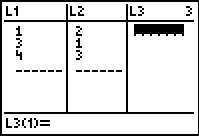
\includegraphics[width=2in]{./LinearQuadraticGraphics/RegData01.jpg} \hspace{0.75in} & 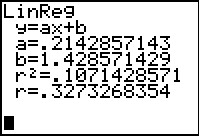
\includegraphics[width=2in]{./LinearQuadraticGraphics/RegLine01.jpg}

\end{tabular}
\end{center}

The calculator tells us that the line of best fit is $y=ax+b$ where the slope is $a \approx 0.214$ and the $y$-coordinate of the $y$-intercept is $b \approx 1.428$.  (We will stick to using three decimal places for our approximations.)  Using this line, we compute the total squared error for our data to be $E \approx 1.786$.  The value $r$ is the \index{regression ! correlation coefficient}\index{correlation coefficient}\textbf{correlation coefficient} and is a measure of how close the data is to being on the same line.  The closer $|r|$ is to $1$, the better the linear fit.  Since $r \approx 0.327$, this tells us that the line of best fit doesn't fit all that well - in other words, our data points aren't close to being linear. The value $r^2$ is called the \index{regression ! coefficient of determination}\index{coefficient of determination}\textbf{coefficient of determination} and is also a measure of the goodness of fit.\footnote{We refer the interested reader to a course in Statistics to explore the significance of $r$ and $r^2$.}  Plotting the data with its regression line results in the picture below.

\begin{center}  

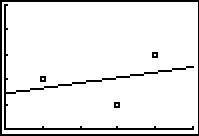
\includegraphics[width=2in]{./LinearQuadraticGraphics/RegLinePlot01.jpg}

\end{center}

Our first example looks at energy consumption in the US over the past 50 years.\footnote{See this \href{http://www.eia.doe.gov/kids/classactivities/EnergyAnalysisEIA.pdf}{\underline{Department of Energy}} activity}

\[\begin{array}{|c|c|} \hline
\mbox{Year} & \mbox{Energy Usage,} \\
& \mbox{ in Quads\footnotemark} \\ \hline
1950 & 34.6 \\ \hline
1960 & 45.1 \\ \hline
1970 & 67.8 \\ \hline
1980 & 78.3 \\ \hline
1990 & 84.6 \\ \hline
2000 & 98.9 \\ \hline

\end{array}\]
\footnotetext{The unit 1 Quad is 1 Quadrillion = $10^{15}$ BTUs, which is enough heat to raise Lake Erie roughly $1^{\circ}$F}

\begin{ex}  \label{energyconsumption}  Using the energy consumption data given above,

\begin{enumerate}

\item  Plot the data using a graphing calculator.

\item  Find the least squares regression line and comment on the goodness of fit.

\item  Interpret the slope of the line of best fit.

\item  Use the regression line to predict the annual US energy consumption in the year $2013$.

\item  Use the regression line to predict when the annual consumption will reach $120$ Quads.

\end{enumerate}

{\bf Solution.}

\begin{enumerate}


\item  Entering the data into the calculator gives

\begin{center}

\begin{tabular}{cc}

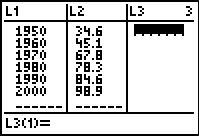
\includegraphics[width=2in]{./LinearQuadraticGraphics/RegData02.jpg} \hspace{0.75in} & 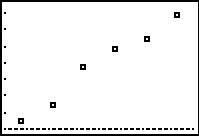
\includegraphics[width=2in]{./LinearQuadraticGraphics/RegDataPlot02.jpg}

\end{tabular}

\end{center}

The data certainly appears to be linear in nature.

\item  Performing a linear regression produces


\begin{center}

\begin{tabular}{cc}

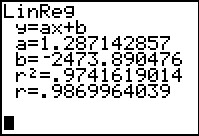
\includegraphics[width=2in]{./LinearQuadraticGraphics/RegLine02.jpg} \hspace{0.75in} & 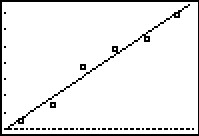
\includegraphics[width=2in]{./LinearQuadraticGraphics/RegLinePlot02.jpg}

\end{tabular}

\end{center}

We can tell both from the correlation coefficient as well as the graph that the regression line is a good fit to the data.

\item  The slope of the regression line is $a \approx 1.287$.  To interpret this, recall that the slope is the rate of change of the $y$-coordinates with respect to the $x$-coordinates.  Since the $y$-coordinates represent the energy usage in Quads, and the $x$-coordinates represent years, a slope of positive $1.287$ indicates an increase in annual energy usage at the rate of $1.287$ Quads per year.

\item  To predict the energy needs in $2013$, we substitute $x=2013$ into the equation of the line of best fit to get  $y = 1.287(2013)-2473.890 \approx 116.841$.  The predicted annual energy usage of the US in $2013$ is approximately $116.841$ Quads.

\item  To predict when the annual US energy usage will reach $120$ Quads, we substitute $y=120$ into the equation of the line of best fit to get $120 = 1.287x - 2473.908$.  Solving for $x$ yields $x \approx 2015.454$.  Since the regression line is increasing, we interpret this result as saying the annual usage in $2015$ won't yet be $120$ Quads, but that in $2016$, the demand will be more than $120$ Quads. \qed

\end{enumerate}
\end{ex}

Our next example gives us an opportunity to find a nonlinear model to fit the data.  According to the National Weather Service, the predicted hourly temperatures for Painesville on March 3, 2009 were given as summarized below.

\[\begin{array}{|c|c|} \hline
\mbox{Time} & \mbox{Temperature, $^{\circ}$F} \\ \hline
10 \mbox{AM} & 17 \\ \hline
11 \mbox{AM} & 19 \\ \hline
12 \mbox{PM} & 21 \\ \hline
1 \mbox{PM} & 23 \\ \hline
2 \mbox{PM} & 24 \\ \hline
3 \mbox{PM} & 24 \\ \hline
4 \mbox{PM} & 23 \\ \hline

\end{array}\]

To enter this data into the calculator, we need to adjust the $x$ values, since just entering the numbers could cause confusion. (Do you see why?)  We have a few options available to us.  Perhaps the easiest is to convert the times into the 24 hour clock time so that $1$ PM is $13$, $2$ PM is $14$, etc..  If we enter these data into the graphing calculator and plot the points we get

\begin{center}

\begin{tabular}{cc}

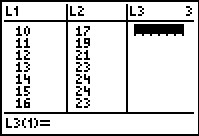
\includegraphics[width=2in]{./LinearQuadraticGraphics/RegData03.jpg} \hspace{0.75in} & 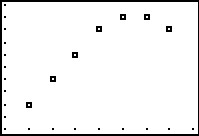
\includegraphics[width=2in]{./LinearQuadraticGraphics/RegPlot03.jpg}

\end{tabular}

\end{center}

While the beginning of the data looks linear, the temperature begins to fall in the afternoon hours.  This sort of behavior reminds us of parabolas, and, sure enough, it is possible to find a parabola of best fit in the same way we found a line of best fit.  The process is called \index{regression ! quadratic}\index{quadratic regression}\textbf{quadratic regression} and its goal is to minimize the least square error of the data with their corresponding points on the parabola.  The calculator has a built in feature for this as well which yields

\begin{center}

\begin{tabular}{cc}

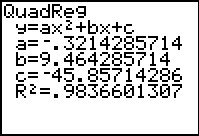
\includegraphics[width=2in]{./LinearQuadraticGraphics/RegPara03.jpg} \hspace{0.75in} & 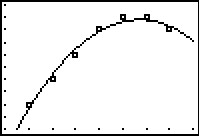
\includegraphics[width=2in]{./LinearQuadraticGraphics/RegParaPlot03.jpg}

\end{tabular}

\end{center}

The coefficient of determination $R^2$ seems reasonably close to $1$, and the graph visually seems to be a decent fit.  We use this model in our next example.

\begin{ex}  Using the quadratic model for the temperature data above, predict the warmest temperature of the day.  When will this occur?

\smallskip

{\bf Solution.}  The maximum temperature will occur at the vertex of the parabola.  Recalling the Vertex Formula, Equation \ref{vertexofquadraticfunctions}, $x = -\frac{b}{2a} \approx - \frac{9.464}{2(-0.321)} \approx 14.741$.  This corresponds to roughly $2\!:\!45$ PM.  To find the temperature, we substitute $x = 14.741$ into $y = -0.321 x^2+9.464x - 45.857$ to get $y \approx 23.899$, or $23.899^{\circ}$F.  \qed

\end{ex}

The results of the last example should remind you that regression models are just that, models.  Our predicted warmest temperature was found to be $23.899^{\circ}$F, but our data says it will warm to $24^{\circ}$F.  It's all well and good to observe trends and guess at a model, but a more thorough investigation into \emph{why} certain data should be linear or quadratic in nature is usually in order - and that, most often, is the business of scientists.

\newpage

\subsection{Exercises}

\begin{enumerate}

\item According to this \href{http://www.ohiobiz.com/census/Lake.pdf}{\underline{website}}\footnote{\href{http://www.ohiobiz.com/census/Lake.pdf}{\underline{http://www.ohiobiz.com/census/Lake.pdf}}}, the census data for Lake County, Ohio is:

\noindent \begin{tabular}{|l|r|r|r|r|} \hline
Year & 1970 & 1980 & 1990 & 2000 \\ 
\hline 
Population & 197200 & 212801 & 215499 & 227511 \\ \hline
\end{tabular}

\begin{enumerate}
 

\item  Find the least squares regression line for these data and comment on the goodness of fit.\footnote{We'll develop more sophisticated models for the growth of populations in Chapter \ref{ExpLogs}.  For the moment, we use a theorem from Calculus to approximate those functions with lines.} Interpret the slope of the line of best fit.

\item  Use the regression line to predict the population of Lake County in 2010.  (The recorded figure from the 2010 census is $230,\!041$)

\item  Use the regression line to predict when the population of Lake County will reach $250,\!000$.

\end{enumerate}


\item According to this \href{http://www.ohiobiz.com/census/Lorain.pdf}{\underline{website}}\footnote{\href{http://www.ohiobiz.com/census/Lorain.pdf}{\underline{http://www.ohiobiz.com/census/Lorain.pdf}}}, the census data for Lorain County, Ohio is:

\noindent \begin{tabular}{|l|r|r|r|r|} \hline
Year & 1970 & 1980 & 1990 & 2000 \\ 
\hline 
Population & 256843 & 274909 & 271126 & 284664 \\ \hline
\end{tabular}

\begin{enumerate}
 

\item  Find the least squares regression line for these data and comment on the goodness of fit. Interpret the slope of the line of best fit.

\item  Use the regression line to predict the population of Lorain County in 2010.  (The recorded figure from the 2010 census is $301,\!356$)

\item  Use the regression line to predict when the population of Lake County will reach $325,\!000$.

\end{enumerate}
\item Using the energy production data given below

\noindent \begin{tabular}{|l|r|r|r|r|r|r|} \hline
Year & 1950 & 1960 & 1970 & 1980 & 1990 & 2000 \\ 
\hline 
Production & & & & & & \\
(in Quads) & 35.6 & 42.8 & 63.5 & 67.2 & 70.7 & 71.2 \\ \hline
\end{tabular}

\begin{enumerate}

\item  Plot the data using a graphing calculator and explain why it does not appear to be linear.

\item  Discuss with your classmates why ignoring the first two data points may be justified from a historical perspective.  

\item Find the least squares regression line for the last four data points and comment on the goodness of fit. Interpret the slope of the line of best fit.

\item  Use the regression line to predict the annual US energy production in the year $2010$.

\item  Use the regression line to predict when the annual US energy production will reach $100$ Quads.

\end{enumerate}


\item The chart below contains a portion of the fuel consumption information for a 2002 Toyota Echo that I (Jeff) used to own.  The first row is the cumulative number of gallons of gasoline that I had used and the second row is the odometer reading when I refilled the gas tank.  So, for example, the fourth entry is the point (28.25, 1051) which says that I had used a total of 28.25 gallons of gasoline when the odometer read 1051 miles.

\medskip

\small

\noindent \begin{tabular}{|l|r|r|r|r|r|r|r|r|r|r|r|} \hline
Gasoline Used & & & & & & & & & & & \\
(Gallons)  & 0 & 9.26 & 19.03 & 28.25 & 36.45 & 44.64 & 53.57 & 62.62 & 71.93 & 81.69 & 90.43\\ 
\hline 
Odometer & & & & & & & & & & & \\
(Miles) & 41 & 356 & 731 & 1051 & 1347 & 1631 & 1966 & 2310 & 2670 & 3030 & 3371\\ \hline
\end{tabular}

\normalsize

\medskip

\noindent Find the least squares line for this data.  Is it a good fit?  What does the slope of the line represent?  Do you and your classmates believe this model would have held for ten years had I not crashed the car on the Turnpike a few years ago?  (I'm keeping a fuel log for my 2006 Scion xA for future College Algebra books so I hope not to crash it, too.)

\item On New Year's Day, I (Jeff, again) started weighing myself every morning in order to have an interesting data set for this section of the book.  (Discuss with your classmates if that makes me a nerd or a geek.  Also, the professionals in the field of weight management strongly discourage weighing yourself every day.  When you focus on the number and not your overall health, you tend to lose sight of your objectives.  I was making a noble sacrifice for science, but you should \underline{not} try this at home.)  The whole chart would be too big to put into the book neatly, so I've decided to give only a small portion of the data to you.  This then becomes a Civics lesson in honesty, as you shall soon see.  There are two charts given below.  One has my weight for the first eight Thursdays of the year (January 1, 2009 was a Thursday and we'll count it as Day 1.) and the other has my weight for the first 10 Saturdays of the year.  

\medskip

\small

\noindent \begin{tabular}{|l|r|r|r|r|r|r|r|r|} \hline
Day \# & & & & & & & &  \\
(Thursday) & 1 & 8 & 15 & 22 & 29 & 36 & 43 & 50 \\ 
\hline 
My weight & & & & & & & & \\
in pounds & 238.2 & 237.0 & 235.6 & 234.4 & 233.0 & 233.8 & 232.8 & 232.0\\ \hline
\end{tabular}

\medskip

\noindent \begin{tabular}{|l|r|r|r|r|r|r|r|r|r|r|} \hline
Day \# & & & & & & & & & & \\
(Saturday) & 3 & 10 & 17 & 24 & 31 & 38 & 45 & 52 & 59 & 66 \\ 
\hline 
My weight & & & & & & & & & & \\
in pounds & 238.4 & 235.8 & 235.0 & 234.2 & 236.2 & 236.2 & 235.2 & 233.2 & 236.8 & 238.2\\ \hline
\end{tabular}

\normalsize

\medskip

\begin{enumerate}

\item Find the least squares line for the Thursday data and comment on its goodness of fit.
\item Find the least squares line for the Saturday data and comment on its goodness of fit.
\item Use Quadratic Regression to find a parabola which models the Saturday data and comment on its goodness of fit.
\item Compare and contrast the predictions the three models make for my weight on January 1, 2010 (Day \#366).  Can any of these models be used to make a prediction of my weight 20 years from now?  Explain your answer.
\item Why is this a Civics lesson in honesty?  Well, compare the two linear models you obtained above.  One was a good fit and the other was not, yet both came from careful selections of real data.  In presenting the tables to you, I have not lied about my weight, nor have you used any bad math to falsify the predictions.  The word we're looking for here is `disingenuous'.  Look it up and then discuss the implications this type of data manipulation could have in a larger, more complex, politically motivated setting.  (Even Obi-Wan presented the truth to Luke only ``from a certain point of view.'')

\end{enumerate}

\item (Data that is neither linear nor quadratic.)  We'll close this exercise set with two data sets that, for reasons presented later in the book, cannot be modeled correctly by lines or parabolas.  It is a good exercise, though, to see what happens when you attempt to use a linear or quadratic model when it's not appropriate.

\begin{enumerate}

\item \label{APLcats} This first data set came from a Summer 2003 publication of the Portage County Animal Protective League called ``Tattle Tails''.  They make the following statement and then have a chart of data that supports it. ``It doesn't take long for two cats to turn into 80 million.  If two cats and their surviving offspring reproduced for ten years, you'd end up with 80,399,780 cats.''  We assume $N(0) = 2$.

\medskip

\scriptsize

\noindent \begin{tabular}{|l|r|r|r|r|r|r|r|r|r|r|} \hline
Year $x$ & 1 & 2 & 3 & 4 & 5 & 6 & 7 & 8 & 9 & 10 \\ 
\hline 
Number of  & & & & & & & & & & \\
Cats $N(x)$ & 12 & 66 & 382 & 2201 & 12680 & 73041 & 420715 & 2423316 & 13968290 & 80399780 \\ \hline
\end{tabular}

\normalsize

\medskip

\noindent Use Quadratic Regression to find a parabola which models this data and comment on its goodness of fit. (Spoiler Alert: Does anyone know what type of function we need here?)

\medskip

\item \label{regsunlight} This next data set comes from the \href{http://aa.usno.navy.mil/data/docs/RS_OneYear.php}{\underline{U.S. Naval Observatory}}.  That site has loads of awesome stuff on it, but for this exercise I used the sunrise/sunset times in Fairbanks, Alaska for 2009 to give you a chart of the number of hours of daylight they get on the $21^{\mbox{st}}$ of each month.  We'll let $x = 1$ represent January 21, 2009, $x = 2$ represent February 21, 2009, and so on.

\medskip

\small

\noindent \begin{tabular}{|l|r|r|r|r|r|r|r|r|r|r|r|r|} \hline
Month  & & & & & & & & & & & & \\
Number & 1 & 2 & 3 & 4 & 5 & 6 & 7 & 8 & 9 & 10 & 11 & 12\\ 
\hline 
Hours of  & & & & & & & & & & & & \\
Daylight & 5.8 & 9.3 & 12.4 & 15.9 & 19.4 & 21.8 & 19.4 & 15.6 & 12.4 & 9.1 & 5.6 & 3.3 \\ \hline
\end{tabular}

\normalsize

\medskip

\noindent Use Quadratic Regression to find a parabola which models this data and comment on its goodness of fit. (Spoiler Alert: Does anyone know what type of function we need here?)

\end{enumerate}

\end{enumerate}

\newpage

\subsection{Answers}

\begin{enumerate}

\item  \begin{enumerate}
 

\item  $y = 936.31x - 1645322.6$ with $r=0.9696$ which indicates a good fit.  The slope $936.31$ indicates Lake County's population is increasing at a rate of (approximately) 936 people per year. 

\item  According to the model, the population in 2010 will be $236, \!660$.

\item  According to the model, the population of Lake County will reach $250,\!000$ sometime between 2024 and 2025.

\end{enumerate}

\item  \begin{enumerate}
 

\item  $y = 796.8x - 1309762.5$ with $r=0.8916$ which indicates a reasonable fit.  The slope $796.8$ indicates Lorain County's population is increasing at a rate of (approximately) 797 people per year. 

\item  According to the model, the population in 2010 will be $291, \! 805$.

\item  According to the model, the population of Lake County will reach $325,\!000$ sometime between 2051 and 2052.

\end{enumerate}

\item \begin{enumerate}

\setcounter{enumii}{2}

\item $y = 0.266x - 459.86$ with $r = 0.9607$ which indicates a good fit.  The slope $0.266$ indicates the country's energy production is increasing at a rate of $0.266$ Quad per year.

\item According to the model, the production in 2010 will be $74.8$ Quad.

\item According to the model, the production will reach $100$ Quad in the year 2105.

\end{enumerate}

\item The line is $y = 36.8x + 16.39$.  We have $r = .99987$ and $r^{2} = .9997$ so this is an excellent fit to the data.  The slope $36.8$ represents miles per gallon.

\item \begin{enumerate}

\item The line for the Thursday data is $y = -.12x + 237.69$.  We have $r = -.9568$ and $r^{2} = .9155$ so this is a really good fit.

\item The line for the Saturday data is $y = -0.000693x + 235.94$.  We have $r = -0.008986$ and $r^{2} = 0.0000807$ which is horrible.  This data is not even close to linear.  

\item The parabola for the Saturday data is $y = 0.003x^{2} - 0.21x + 238.30$.  We have $R^{2} = .47497$ which isn't good.  Thus the data isn't modeled well by a quadratic function, either.

\item The Thursday linear model had my weight on January 1, 2010 at 193.77 pounds.  The Saturday models give 235.69 and 563.31 pounds, respectively.  The Thursday line has my weight going below 0 pounds in about five and a half years, so that's no good.  The quadratic has a positive leading coefficient which would mean unbounded weight gain for the rest of my life.  The Saturday line, which mathematically does not fit the data at all, yields a plausible weight prediction in the end.  I think this is why grown-ups talk about ``Lies, Damned Lies and Statistics.''

\end{enumerate}

\item \begin{enumerate}

\item The quadratic model for the cats in Portage county is $y = 1917803.54x^{2} - 16036408.29x + 24094857.7$.  Although $R^{2} = .70888$ this is not a good model because it's so far off for small values of $x$.  Case in point, the model gives us 24,094,858 cats when $x = 0$ but we know $N(0) = 2$.

\item The quadratic model for the hours of daylight in Fairbanks, Alaska is $y = .51x^{2} + 6.23x - .36$.  Even with $R^{2} = .92295$ we should be wary of making predictions beyond the data.  Case in point, the model gives $-4.84$ hours of daylight when $x = 13$.  So January 21, 2010 will be ``extra dark''?  Obviously a parabola pointing down isn't telling us the whole story.

\end{enumerate}

\end{enumerate}


\closegraphsfile

\newpage

\end{document}